% PREAMBLE
\documentclass[11pt, a4paper]{report}
\usepackage[utf8]{inputenc}
\usepackage{amsmath, amssymb, amsfonts}
\usepackage{graphicx, geometry, hyperref, fancyhdr, titlesec, xcolor}
\usepackage{tikz}
\usepackage{float}
\usetikzlibrary{decorations.pathmorphing, decorations.markings, arrows.meta, calc}
\geometry{margin=0.8in}

\hypersetup{
colorlinks=true,
linkcolor=blue,
urlcolor=blue,
citecolor=blue
}

\titleformat{\chapter}[display]{\normalfont\Large\bfseries}{\chaptertitlename\ \thechapter}{1em}{}
\titlespacing*{\chapter}{0pt}{5pt}{15pt}
\titleformat{\section}{\normalfont\Large\bfseries\itshape}{\thesection}{1em}{}
\titleformat{\subsection}{\normalfont\large\itshape}{\thesubsection}{1em}{}
\titleformat{\subsubsection}{\normalfont\normalsize\itshape}{\thesubsubsection}{1em}{}

\pagestyle{fancy}
\fancyhf{}
\fancyhead[L]{\nouppercase{\leftmark}}
\fancyfoot[C]{\thepage}
\renewcommand{\headrulewidth}{1pt}
\renewcommand{\footrulewidth}{1pt}

\begin{document}
\begin{titlepage}
    \begin{center}
        \vspace*{28.45pt}
            
        \Huge
        \textbf{Foundations of General Relativity: From Flat Spacetime to the Schwarzschild Solution}
            
        \vspace{14.23pt}
        \LARGE
        A Mathematical and Geometric Approach to Gravitation
            
        \vspace{42.68pt}
            
        \textbf{Abdelrahman Mohamed Anwar}
            
        \vspace{28.45pt}
        
        \Large
        Supervised by\\
        \textbf{Prof. Dr. Elsayed Lashin}
            
        \vfill
            
        \Large
        A thesis presented for the degree of\\
        Bachelor of Science
            
        \vspace{22.76pt}
            
        \Large
        Department of Physics\\
        Ain Shams University\\
        2026
            
    \end{center}
\end{titlepage}

\newpage
\thispagestyle{empty}

\begin{abstract}
This thesis provides a comprehensive, mathematically rigorous review of General Relativity, tracing the theoretical development from the postulates of flat spacetime to the exact solutions of Einstein's field equations. We begin by formalizing Special Relativity using four-vector formalism and analyzing causality through the light cone structure. The mathematical framework of pseudo-Riemannian manifolds, tensor calculus, and differential forms is then systematically developed to describe curved spacetime. Utilizing the Einstein Equivalence Principle and minimal coupling, we derive the geodesic equation and Einstein's field equations, including discussions on the Newtonian limit, the Hilbert action, and the various energy conditions. Finally, we rigorously derive the Schwarzschild solution for a static, spherically symmetric vacuum. The causal structure of the Schwarzschild black hole is examined using Eddington-Finkelstein coordinates, and the classical experimental tests of General Relativity—specifically the precession of the perihelion and gravitational redshift—are analyzed. This work serves as a foundational synthesis of the geometric approach to gravitation, establishing the necessary groundwork for advanced studies in theoretical cosmology and high-energy physics.
\end{abstract}

\newpage
\tableofcontents
\newpage

\newcommand{\eqn}[1]{\hyperref[#1]{\eqref{#1}}}

\chapter*{Conventions and Notation}
\addcontentsline{toc}{chapter}{Conventions and Notation}

This thesis strictly adheres to the mathematical conventions and notation established in Sean M. Carroll's \textit{Spacetime and Geometry: An Introduction to General Relativity}. The primary conventions utilized throughout the following chapters are detailed below.

\section*{Units}
We adopt \textbf{natural units}, which are customary in high-energy physics and theoretical cosmology. In this system, the speed of light in a vacuum, $c$, and Newton's gravitational constant, $G$, are set to unity:
\begin{equation}
c = G = 1
\end{equation}
Consequently, mass, length, and time all share the same physical dimensions. When necessary for physical clarity or when evaluating experimental tests, $c$ and $G$ may be explicitly reintroduced.

\section*{Metric Signature}
We employ the "mostly plus" metric signature, common in particle physics and modern relativity texts. The flat Minkowski metric $\eta_{\mu\nu}$ is defined as:
\begin{equation}
\eta_{\mu\nu} = \text{diag}(-1, +1, +1, +1)
\end{equation}
Correspondingly, timelike intervals satisfy $ds^2 < 0$, spacelike intervals satisfy $ds^2 > 0$, and null intervals satisfy $ds^2 = 0$.

\section*{Index Notation}
The Einstein summation convention is used throughout, wherein repeated indices (one upper, one lower) are implicitly summed over.
\begin{itemize}
    \item \textbf{Greek indices} ($\mu, \nu, \rho, \sigma, \dots$) represent full spacetime components and range over $0, 1, 2, 3$, where $0$ denotes the time coordinate.
    \item \textbf{Latin indices} ($i, j, k, l, \dots$) represent purely spatial components and range over $1, 2, 3$.
    \item \textbf{Hatted indices} ($\hat{\mu}, \hat{\nu}, \dots$) denote components evaluated in a localized, orthonormal basis (e.g., tetrad or locally inertial frames), as opposed to a general coordinate basis.
\end{itemize}

\section*{Curvature Sign Conventions}
The sign conventions for curvature tensors are notoriously varied across the literature. This thesis adopts the following definitions:

\textbf{1. The Riemann Curvature Tensor:}
Defined via the commutator of covariant derivatives acting on a dual vector, $[\nabla_\mu, \nabla_\nu] V^\rho = {R^\rho}_{\sigma\mu\nu} V^\sigma$. In terms of the Christoffel connection, this evaluates to:
\begin{equation}
{R^\rho}_{\sigma\mu\nu} = \partial_{\mu}\Gamma^{\rho}_{\nu\sigma} - \partial_{\nu}\Gamma^{\rho}_{\mu\sigma} + \Gamma^{\rho}_{\mu\lambda}\Gamma^{\lambda}_{\nu\sigma} - \Gamma^{\rho}_{\nu\lambda}\Gamma^{\lambda}_{\mu\sigma}
\end{equation}

\textbf{2. The Ricci Tensor and Scalar:}
The Ricci tensor is the unique non-vanishing trace of the Riemann tensor, defined by contracting the first and third indices:
\begin{equation}
R_{\mu\nu} = {R^\lambda}_{\mu\lambda\nu}
\end{equation}
The Ricci scalar is the trace of the Ricci tensor: $R = g^{\mu\nu}R_{\mu\nu}$.

\textbf{3. The Einstein Field Equations:}
With the above conventions, and applying the minimal coupling principle to the Hilbert action, the Einstein Field Equations take the form:
\begin{equation}
R_{\mu\nu} - \frac{1}{2}R g_{\mu\nu} = 8\pi T_{\mu\nu}
\end{equation}
where $T_{\mu\nu}$ is the energy-momentum tensor. (Note the positive sign on the right-hand side, a direct consequence of the $(- + + +)$ metric signature and the specific contraction used for the Ricci tensor).


% ==========================================
% INTRODUCTION CHAPTER
% ==========================================

\chapter{Introduction}

Gravity is the most familiar of the fundamental forces, yet historically, it has been the most difficult to conceptualize. For over two centuries, Newton's law of universal gravitation reigned supreme, modeling gravity as an instantaneous, invisible tether connecting massive bodies across absolute space and absolute time. While this formulation was phenomenally successful in describing planetary orbits and terrestrial mechanics, it harbored fatal incompatibilities with the framework of special relativity introduced by Albert Einstein in 1905. Special relativity dismantled the notions of absolute space and absolute time, proving that no signal—not even the force of gravity—could propagate faster than the speed of light.
\newline

General Relativity, finalized by Einstein in 1915, elegantly resolved this tension not by modifying Newton's force law, but by eliminating the concept of gravitational "force" entirely. Instead, general relativity posits a profound conceptual leap: gravity is the manifestation of the curvature of spacetime. Massive bodies do not pull on one another; rather, they warp the very fabric of the four-dimensional manifold they inhabit, and in turn, the geometry of this manifold dictates how matter must move. In the words of John Archibald Wheeler, "Spacetime tells matter how to move; matter tells spacetime how to curve."
\newline

This thesis aims to explore the rigorous mathematical foundations and physical implications of general relativity. The journey from flat space to curved geometry requires a robust mathematical toolkit, which we will systematically build. 
\newline

We begin in \textbf{Chapter 1} by reviewing Special Relativity and the geometry of flat Minkowski spacetime, establishing the language of tensors and four-vectors that will be generalized later. 
In \textbf{Chapter 2}, we introduce the mathematics of differentiable manifolds, formally generalizing calculus to curved spaces and establishing the Equivalence Principle as the physical bridge between coordinate systems. 
\textbf{Chapter 3} delves into the heart of differential geometry, rigorously defining the covariant derivative, parallel transport, geodesics, and the Riemann curvature tensor—the ultimate measure of spacetime deviation from flatness.
In \textbf{Chapter 4}, we transition from pure geometry to physics, deriving the Einstein Field Equations from both heuristic physical arguments and the rigorous Lagrangian formalism of the Einstein-Hilbert action.
Finally, in \textbf{Chapter 5}, we explore the most famous exact solution to these field equations: the Schwarzschild metric. By analyzing this solution, we will uncover the theoretical existence of black holes, the precession of planetary orbits, and the absolute causal boundaries known as event horizons.
\newline

By navigating these chapters, this thesis will demonstrate how general relativity weaves the mechanics of the cosmos into a unified, exquisitely beautiful geometric tapestry.



\chapter{Special Relativity and Flat Spacetime}

\section{Prelude}

\subsection*{Core Concept of General Relativity}
The foundational postulate of general relativity is the geometric conceptualization of gravity. Rather than treating gravity as a conventional force propagating through an inert background, the theory models it as a physical manifestation of spacetime curvature dynamically responding to the presence of mass and energy.

\subsection*{Newtonian Gravity: A Review}
In classical mechanics, gravity is modeled as an instantaneous, action-at-a-distance force between massive bodies. Mathematically, this is expressed through Newton's law of universal gravitation and his second law of motion:
\begin{equation}\label{eq:newton-force}
F = - \frac{GMm}{r^2} \hat{e}_r
\end{equation}
\begin{equation}\label{eq:newton-second}
F = ma
\end{equation}

While the vector formulation is intuitive, it is physically more illuminating to describe the gravitational field mathematically as the gradient of a scalar potential, $\Phi$. By evaluating the gravitational flux over a closed surface bounding the source volume and applying Gauss's theorem, the relationship between local mass density $\rho$ and the potential is established. This geometric formulation eliminates non-local dependencies, yielding Poisson's equation:
\begin{equation}\label{eq:poisson}
\nabla^2 \Phi = 4\pi G \rho
\end{equation}
\begin{equation}\label{eq:potential-accel}
a = -\nabla \Phi
\end{equation}

\subsection*{General Relativity: A Preview}
General relativity completely overhauls the Newtonian paradigm. Geometrically, mass-energy distributions induce a curvature in the spacetime manifold. This dynamic relationship between geometry and matter is governed by the Einstein field equations, where the Einstein tensor $R_{\mu\nu} - \frac{1}{2} R g_{\mu\nu}$ dictates the curvature and the energy-momentum tensor $T_{\mu\nu}$ represents the source:
\begin{equation}\label{eq:einstein}
R_{\mu\nu} - \frac{1}{2} R g_{\mu\nu} = 8\pi G T_{\mu\nu}
\end{equation}
In the absence of non-gravitational forces, test particles travel along the "straightest" possible paths in this curved manifold, known as geodesics. Mathematically, this trajectory minimizes the proper time and is governed by the geodesic equation:
\begin{equation}\label{eq:geodesic}
\frac{d^2 x^{\mu}}{d\lambda^2} + \Gamma^{\mu}_{\rho\sigma} \frac{dx^{\rho}}{d\lambda} \frac{dx^{\sigma}}{d\lambda} = 0
\end{equation}

\section{Space and Time, Separately and Together}
The transition to special relativity requires abandoning the notion of absolute simultaneity. Space and time are fundamentally interwoven into a single four-dimensional mathematical structure known as Minkowski spacetime. 

\subsection*{Spacetime and Worldlines}
Physically, a point in this continuum is an \emph{event}, defined by specific spatial and temporal coordinates. The history of a particle moving through spacetime traces out a continuous one-dimensional curve referred to as its \emph{worldline}.

\subsection*{Relativistic Spacetime: The Light Cone Structure}
Because the speed of light is invariant across all inertial reference frames, the causal structure of spacetime is strictly bounded. Geometrically, this boundary forms a \emph{light cone} at every event, cleanly dividing spacetime into regions that can be causally affected by the event (the future light cone) and regions that could have influenced it (the past light cone). 

\begin{figure}[htbp]
\centering
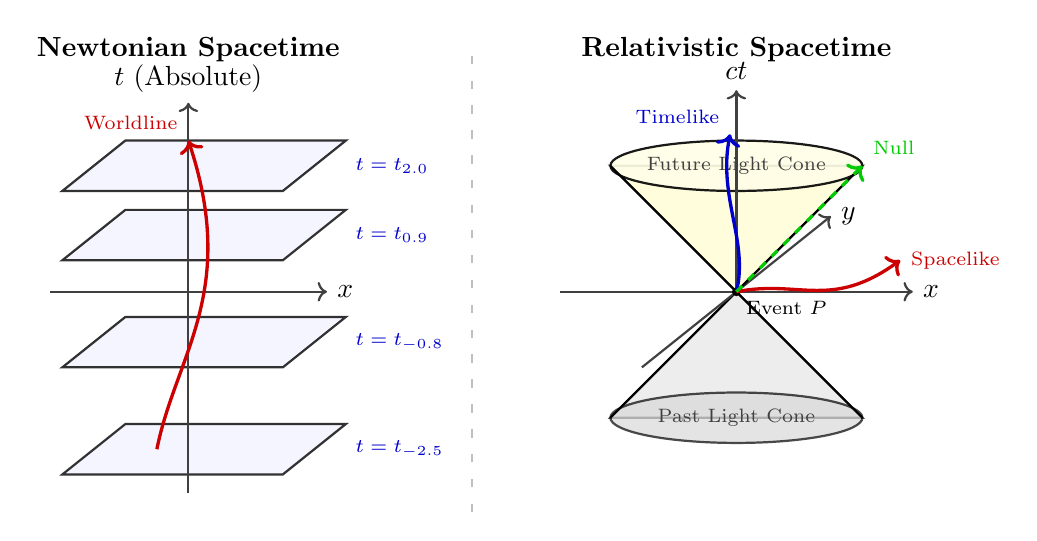
\begin{tikzpicture}[scale=0.8]
  % ----- Left: Newtonian Spacetime -----
  \begin{scope}[shift={(-4.5, 0)}]
    \node[above, font=\bfseries] at (0, 3.5) {Newtonian Spacetime};
    
    % Planes of absolute simultaneity
    \foreach \y in {-2.5, -0.8, 0.9, 2.0} {
      \draw[thick, fill=blue!5, opacity=0.8] (-2, \y-0.4) -- (1.5, \y-0.4) -- (2.5, \y+0.4) -- (-1, \y+0.4) -- cycle;
      \node[right, blue!80!black, font=\scriptsize] at (2.5, \y) {$t = t_{\y}$};
    }
    
    % Axes
    \draw[->, thick, darkgray] (0,-3.2) -- (0, 3.0) node[above, text=black] {$t$ (Absolute)};
    \draw[->, thick, darkgray] (-2.2,0) -- (2.2, 0) node[right, text=black] {$x$};
    
    % Particle worldline
    \draw[very thick, red!80!black, ->] (-0.5, -2.5) .. controls (-0.2, -1) and (0.8, 0) .. (0.0, 2.4) node[above left, font=\scriptsize] {Worldline};
  \end{scope}

  % ----- Divider -----
  \draw[thick, loosely dashed, gray!50] (0, -3.5) -- (0, 4);

  % ----- Right: Relativistic Spacetime -----
  \begin{scope}[shift={(4.2, 0)}]
    \node[above, font=\bfseries] at (0, 3.5) {Relativistic Spacetime};
    
    % Past Light Cone
    \draw[thick, fill=gray!20, opacity=0.7] (-2,-2) -- (0,0) -- (2,-2) -- cycle;
    \draw[thick, fill=gray!30, opacity=0.7] (0,-2) ellipse (2 and 0.4);
    \draw[thick] (-2,-2) -- (0,0) -- (2,-2);
    
    % Axes (drawn behind future cone, over past cone)
    \draw[->, thick, darkgray] (-2.8,0) -- (2.8, 0) node[right, text=black] {$x$};
    \draw[->, thick, darkgray] (-1.5,-1.2) -- (1.5, 1.2) node[right, text=black] {$y$};
    
    % Future Light Cone
    \draw[thick, fill=yellow!20, opacity=0.7] (-2,2) -- (0,0) -- (2,2) -- cycle;
    \draw[thick, fill=yellow!10, opacity=0.9] (0,2) ellipse (2 and 0.4);
    \draw[thick] (-2,2) -- (0,0) -- (2,2);
    \draw[->, thick, darkgray] (0,0) -- (0, 3.2) node[above, text=black] {$ct$};
    
    % Labels for regions
    \node[font=\scriptsize, darkgray] at (0, -2) {Past Light Cone};
    \node[font=\scriptsize, darkgray] at (0, 2) {Future Light Cone};

    % Origin Event
    \fill[black] (0,0) circle (2pt) node[below right, font=\scriptsize] {Event $P$};

    % Causal Structure Worldlines
    % Timelike
    \draw[very thick, blue!80!black, ->] (0,0) .. controls (0.2, 0.8) and (-0.3, 1.5) .. (-0.1, 2.5) node[above left, font=\scriptsize] {Timelike};
    % Spacelike
    \draw[very thick, red!80!black, ->] (0,0) .. controls (1, 0.2) and (1.5, -0.3) .. (2.6, 0.5) node[right, font=\scriptsize] {Spacelike};
    % Null (on the cone)
    \draw[very thick, green!80!black, dashed, ->] (0,0) -- (2, 2) node[above right, font=\scriptsize] {Null};
  \end{scope}

\end{tikzpicture}
\caption{Comparison of Newtonian absolute spacetime (left) and Minkowskian causal structure (right), showing the past/future light cones of event $P$ and its causal regions.}
\label{fig:spacetime_comparison}
\end{figure}


\subsection*{The Invariant Spacetime Interval}
The primary geometric invariant in special relativity is the spacetime interval. Just as the Euclidean distance between two points remains unchanged under spatial rotations, the spacetime interval remains identical for all inertial observers, regardless of their relative velocities. Using the signature convention $(- + + +)$ and natural units ($c=1$), the flat spacetime metric is defined as:
\begin{equation}\label{eq:minkowski-metric}
\eta_{\mu\nu} = \text{diag}(-1, 1, 1, 1)
\end{equation}

\subsection*{Causal Structure and Proper Time}
The sign of the invariant interval classifies the geometric relationship between events:
\begin{itemize}
\item \textbf{Timelike:} $(\Delta s)^2 < 0$ (Events can be causally linked by massive particles).
\item \textbf{Spacelike:} $(\Delta s)^2 > 0$ (Events are causally disconnected).
\item \textbf{Null:} $(\Delta s)^2 = 0$ (Events are connected by massless particles, e.g., photons).
\end{itemize}
For a timelike trajectory, the interval provides a measure of \emph{proper time} $\tau$---the time recorded by a clock physically transported along the worldline:
\begin{equation}\label{eq:proper-time}
(\Delta \tau)^2 = -(\Delta s)^2 = -\eta_{\mu\nu} \Delta x^\mu \Delta x^\nu
\end{equation}

For a general arbitrary trajectory parameterized by $\lambda$, integrating the infinitesimal contributions yields the total proper time:
\begin{equation}
\Delta \tau = \int \sqrt{ -\eta_{\mu\nu} \frac{dx^\mu}{d\lambda} \frac{dx^\nu}{d\lambda} } d\lambda
\end{equation}

\section{Lorentz Transformations}
To maintain the invariance of physical laws, coordinate transformations between inertial frames must leave the Minkowski metric unchanged.

\subsection*{Translations and Linear Transformations}
The most general transformations include spacetime translations (shifting the origin) and linear transformations (rotations and boosts):
\begin{equation}\label{eq:translation}
x^{\mu'} = \delta^{\mu'}_\mu (x^\mu + a^\mu)
\end{equation}
\begin{equation}\label{eq:linear-transform}
x^{\mu'} = {\Lambda^{\mu'}}_\nu x^\nu
\end{equation}

\subsection*{Condition for Lorentz Transformation}
Imposing the condition that the spacetime interval $(\Delta s)^2$ is preserved geometrically constrains the transformation matrix $\Lambda$. These constraints define the Lorentz group $\text{O}(3,1)$:
\begin{equation}\label{eq:lorentz-condition}
\eta = \Lambda^T \eta \Lambda \quad \text{or} \quad \eta_{\rho\sigma} = {\Lambda^{\mu'}}_\rho {\Lambda^{\nu'}}_\sigma \eta_{\mu'\nu'}
\end{equation}

\subsection*{Explicit Transformation Matrices}
The Lorentz group includes standard spatial rotations, such as a rotation within the $x-y$ plane:
\begin{equation}\label{eq:rotation-matrix}
{\Lambda^{\mu'}}_{\nu} =
\begin{pmatrix}
1 & 0 & 0 & 0 \\
0 & \cos\theta & \sin\theta & 0 \\
0 & -\sin\theta & \cos\theta & 0 \\
0 & 0 & 0 & 1
\end{pmatrix}
\end{equation}

It also incorporates Lorentz boosts, which relate frames moving at a constant relative velocity. Geometrically, a boost acts as a hyperbolic rotation in spacetime. For a boost along the $x$-direction parameterized by the rapidity $\phi$:
\begin{equation}\label{eq:boost-matrix}
{\Lambda^{\mu'}}_{\nu} =
\begin{pmatrix}
\cosh\phi & -\sinh\phi & 0 & 0 \\
-\sinh\phi & \cosh\phi & 0 & 0 \\
0 & 0 & 1 & 0 \\
0 & 0 & 0 & 1
\end{pmatrix}
\end{equation}
Substituting physical kinematic variables $v = \tanh\phi$ and the Lorentz factor $\gamma = 1/\sqrt{1-v^2}$ recovers the standard Lorentz coordinate transformations:
\begin{align}
t' &= \gamma(t - vx) \label{eq:lorentz-tprime} \\
x' &= \gamma(x - vt) \label{eq:lorentz-xprime}
\end{align}

\section{Vectors}
In the rigorous framework of differential geometry, vectors are not viewed merely as directed arrows in space, but as directional derivatives evaluated at a point. Physically, they inhabit the \emph{tangent space} $T_p$ constructed at a specific spacetime event $p$.

\begin{figure}[htbp]
\centering
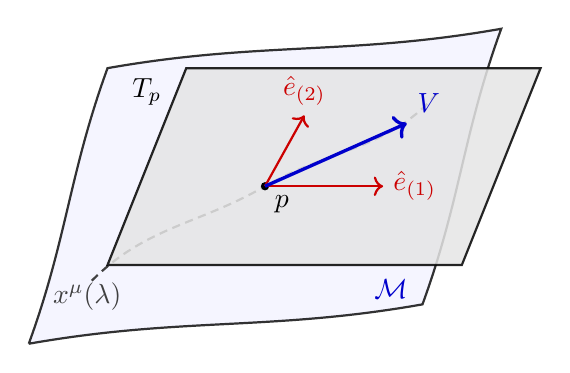
\begin{tikzpicture}[scale=1.0]
  % Define the center point p
  \coordinate (P) at (3, 2);

  % Draw the curved manifold (surface M)
  \draw[thick, fill=blue!5, opacity=0.8] 
    (0,0) to[out=10, in=190] (5,0.5) 
          to[out=70, in=250] (6,4) 
          to[out=190, in=10] (1,3.5) 
          to[out=250, in=70] (0,0);
  \node[blue!80!black] at (4.6, 0.7) {$\mathcal{M}$};

  % Draw a curve x^\mu(\lambda) on the manifold passing through p
  \draw[thick, densely dashed, darkgray] 
    (0.8, 0.8) to[out=45, in=210] (P) to[out=30, in=230] (5.2, 3.2);
  \node[darkgray, above left] at (1.3, 0.3) {$x^\mu(\lambda)$};

  % Draw the tangent plane T_p at point p
  \draw[thick, fill=gray!20, opacity=0.85] 
    (1, 1) -- (5.5, 1) -- (6.5, 3.5) -- (2, 3.5) -- cycle;
  \node at (1.5, 3.2) {$T_p$};

  % Mark the point p
  \fill[black] (P) circle (1.5pt) node[below right] {$p$};

  % Basis vectors e_(\mu) on the tangent plane
  \draw[->, thick, red!80!black] (P) -- ++(1.5, 0) node[right] {$\hat{e}_{(1)}$};
  \draw[->, thick, red!80!black] (P) -- ++(0.5, 0.9) node[above] {$\hat{e}_{(2)}$};

  % Tangent vector V^\mu = dx^\mu / d\lambda
  \draw[->, very thick, blue!80!black] (P) -- ++(1.8, 0.8) node[above right] {$V$};

\end{tikzpicture}
\caption{Geometric representation of a curve $x^\mu(\lambda)$ and its tangent vector $V^\mu$ in the local tangent space $T_p$ of a manifold $\mathcal{M}$.}
\label{fig:tangent_space}
\end{figure}

\subsection*{Basis and Transformation}
A vector $A = A^\mu \hat{e}_{(\mu)}$ is an invariant geometric object. For a curve parametrized by $\lambda$, the tangent vector is naturally defined as $V^\mu = dx^\mu/d\lambda$. Under a change of coordinates, the vector components transform contravariantly via $\Lambda$, while the basis vectors transform covariantly (via the inverse matrix) to guarantee that the geometric vector itself remains invariant:
\begin{equation}
V^{\mu'} = {\Lambda^{\mu'}}_\nu V^\nu
\end{equation}
\begin{equation}
\hat{e}_{(\nu')} = {\Lambda^\mu}_{\nu'} \hat{e}_{(\mu)}
\end{equation}

\section{Dual Vectors (One-Forms)}
Corresponding to every tangent space $T_p$ is a dual space, known as the \emph{cotangent space} $T_p^*$. The elements of this space are dual vectors (or one-forms). Geometrically, a one-form can be conceptualized as a series of parallel hyperplanes, and its action on a vector corresponds to the number of hyperplanes the vector pierces. 

\subsection*{Basis and Action}
Mathematically, a dual vector $\omega$ is a linear functional mapping vectors to real numbers. The dual basis vectors $\hat{\theta}^{(\nu)}$ are defined such that their action on the tangent basis vectors yields the Kronecker delta: $\hat{\theta}^{(\nu)}(\hat{e}_{(\mu)}) = \delta^\nu_\mu$. Contracting a dual vector $\omega = \omega_\mu \hat{\theta}^{(\mu)}$ with a vector $V$ produces an invariant scalar:
\begin{equation}
\omega(V) = \omega_\mu V^\mu \in \mathbb{R}
\end{equation}

\subsection*{Transformation and Gradient}
Because dual vectors map contravariant vectors to invariant scalars, their components must transform via the inverse Lorentz matrix:
\begin{equation}
\omega_{\mu'} = {\Lambda^\nu}_{\mu'} \omega_\nu
\end{equation}
The most prominent physical example of a dual vector is the gradient of a scalar field, $d\phi = \partial_\mu \phi \hat{\theta}^{(\mu)}$, demonstrating standard covariant transformation properties:
\begin{equation}
\frac{\partial\phi}{\partial x^{\mu'}} = {\Lambda^\nu}_{\mu'} \frac{\partial\phi}{\partial x^\nu}
\end{equation}

\section{Tensors}
Tensors represent a generalization of vectors and dual vectors, operating as multilinear machines that map sets of vectors and dual vectors into real numbers. 

\subsection*{Tensor Components}
A tensor of type $(k, l)$ is constructed via the tensor product $\otimes$ of $k$ vectors and $l$ dual vectors. Its components transform under coordinate changes through a combination of contravariant and covariant Lorentz matrices:
\begin{equation}
{T^{\mu'_1 \dots \mu'_k}}_{\nu'_1 \dots \nu'_l} = {\Lambda^{\mu'_1}}_{\mu_1} \dots {\Lambda^{\nu_l}}_{\nu'_l} {T^{\mu_1 \dots \mu_k}}_{\nu_1 \dots \nu_l}
\end{equation}

\subsection*{Spacetime Tensors}
Several fundamental tensors characterize the structure of spacetime and physical fields within it:
\begin{itemize}
\item \textbf{Metric Tensor ($\eta_{\mu\nu}$):} Defines distances and angles; $\eta(V, W) = \eta_{\mu\nu}V^\mu W^\nu$.
\item \textbf{Inverse Metric ($\eta^{\mu\nu}$):} Defined algebraically via $\eta^{\mu\rho}\eta_{\rho\nu} = \delta^\mu_\nu$.
\item \textbf{Levi-Civita Tensor ($\tilde{\epsilon}_{\mu\nu\rho\sigma}$):} The totally antisymmetric volume element.
\item \textbf{Electromagnetic Field Tensor ($F_{\mu\nu}$):} A rank-2 antisymmetric tensor unifying the electric and magnetic vector fields into a single geometric entity:
\begin{equation}\label{eq:EM Field Tensor}
F_{\mu\nu} =
\begin{pmatrix}
0 & -E_1 & -E_2 & -E_3 \\
E_1 & 0 & B_3 & -B_2 \\
E_2 & -B_3 & 0 & B_1 \\
E_3 & B_2 & -B_1 & 0
\end{pmatrix}
= -F_{\nu\mu}
\end{equation}
\end{itemize}

\section{Manipulating Tensors}
The index notation provides a robust methodology for tensor algebra, ensuring structural integrity during calculations. The operation of \textbf{contraction} sums over one upper and one lower index, generating a tensor of lower rank. The metric tensor functions geometrically to map vectors to their duals and vice versa, executing \textbf{raising and lowering} of indices:
\begin{align}
{T^{\alpha\beta\mu}}_\delta &= \eta^{\mu\gamma} {T^{\alpha\beta}}_{\gamma\delta} \\
V_\mu &= \eta_{\mu\nu}V^\nu
\end{align}
The \textbf{trace} is simply the full contraction of a tensor with the metric, producing a scalar: $X = {X^\lambda}_\lambda = \eta^{\mu\nu}Y_{\mu\nu}$.

\section{Maxwell's Equations}
By expressing electromagnetism in terms of the field tensor $F_{\mu\nu}$, Maxwell's equations can be written in a manifestly covariant form. This geometric structure guarantees their validity across all inertial reference frames.

Applying the four-divergence to the field tensor yields the inhomogeneous equations (Gauss's law and the Ampère-Maxwell law), directly relating the fields to the four-current source $J^\nu$:
\begin{equation}\label{eq:inhom-maxwell}
\partial_\mu F^{\nu\mu} = J^\nu
\end{equation}
The homogeneous equations (Faraday's law and the absence of magnetic monopoles) dictate that the totally antisymmetric derivative of the field tensor vanishes identically:
\begin{equation}\label{eq:hom-maxwell}
\partial_{[\mu} F_{\nu\lambda]} = 0 \quad \implies \quad \partial_\mu F_{\nu\lambda} + \partial_\nu F_{\lambda\mu} + \partial_\lambda F_{\mu\nu} = 0
\end{equation}

\section{Energy and Momentum}
Relativistic mechanics requires reformulating energy and momentum as components of covariant geometric objects. 

\subsection*{Four-Velocity and Four-Momentum}
The four-velocity $U^\mu$ is the tangent vector to a particle's worldline parameterized by proper time. The mass of the particle, an invariant scalar, scales this vector to produce the four-momentum $p^\mu$, naturally unifying energy and classical 3-momentum:
\begin{equation}
U^\mu = \frac{dx^\mu}{d\tau}, \quad \eta_{\mu\nu}U^\mu U^\nu = -1
\end{equation}
\begin{equation}
p^\mu = mU^\mu, \quad p_\mu p^\mu = -m^2 \implies E = \sqrt{m^2 + p^2}
\end{equation}

\subsection*{Four-Force}
Dynamics are described by the four-force, which dictates the rate of change of proper momentum. For instance, the Lorentz force law is purely geometric when utilizing the electromagnetic tensor:
\begin{equation}
f^\mu = \frac{dp^\mu}{d\tau} = q {F^\mu}_\lambda U^\lambda
\end{equation}

\subsection*{Energy-Momentum Tensor $T^{\mu\nu}$}
For continuous distributions of matter, physical properties are captured by the energy-momentum tensor $T^{\mu\nu}$, representing the flux of the $\mu$-component of momentum across a surface of constant $\nu$. 

For a simple "dust" (a pressureless fluid of non-interacting particles with number density $n$ and rest mass density $\rho$), $T^{\mu\nu} = \rho U^\mu U^\nu$. Applying a Lorentz transformation matrix yields its components in an arbitrary inertial frame moving with velocity vector $\mathbf{v}$:
\begin{equation}
T^{\mu'\nu'} = \rho \gamma^2
\begin{pmatrix}
1 & -v_x & -v_y & -v_z \\
-v_x & v_x^2 & v_x v_y & v_x v_z \\
-v_y & v_y v_x & v_y^2 & v_y v_z \\
-v_z & v_z v_x & v_z v_y & v_z^2
\end{pmatrix}
\end{equation}

For a more realistic perfect fluid incorporating isotropic pressure $p$, the tensor must be modified to include spatial momentum fluxes:
\begin{equation}
T^{\mu\nu} = (\rho+p)U^\mu U^\nu + p\eta^{\mu\nu}
\end{equation}
Transforming this tensor to a laboratory frame yields:
\begin{equation}
T^{\mu'\nu'} =
\begin{pmatrix}
\gamma^2(\rho + p) - p & -\gamma^2 v_x (\rho + p) & -\gamma^2 v_y (\rho + p) & -\gamma^2 v_z (\rho + p) \\
-\gamma^2 v_x (\rho + p) & \gamma^2 v_x^2 (\rho + p) + p & \gamma^2 v_x v_y (\rho + p) & \gamma^2 v_x v_z (\rho + p) \\
-\gamma^2 v_y (\rho + p) & \gamma^2 v_y v_x (\rho + p) & \gamma^2 v_y^2 (\rho + p) + p & \gamma^2 v_y v_z (\rho + p) \\
-\gamma^2 v_z (\rho + p) & \gamma^2 v_z v_x (\rho + p) & \gamma^2 v_z v_y (\rho + p) & \gamma^2 v_z^2 (\rho + p) + p
\end{pmatrix}
\end{equation}

\subsection*{Conservation Law}
The conservation of energy and momentum in flat spacetime is dictated by the vanishing divergence of $T^{\mu\nu}$:
\begin{equation}\label{eq:cons-T}
\partial_\mu T^{\mu\nu} = 0
\end{equation}
Expanding the divergence of the perfect fluid energy-momentum tensor and projecting the result orthogonal and parallel to the four-velocity $U^\mu$ recovers the relativistic analogues of the Euler equation (momentum conservation) and the continuity equation (energy conservation), respectively.

\section{Classical Field Theory}
\subsection*{Euler-Lagrange Equations}
A rigorous foundation for field theory relies on the principle of stationary action. By defining an invariant scalar Lagrangian density $\mathcal{L}$ for fields $\Phi^i$, setting the variation of the action $S = \int \mathcal{L} d^4x$ to zero yields the Euler-Lagrange equations:
\begin{equation}
\frac{\partial\mathcal{L}}{\partial\Phi^i} - \partial_\mu\left(\frac{\partial\mathcal{L}}{\partial(\partial_\mu\Phi^i)}\right) = 0
\end{equation}

Applying the Euler-Lagrange framework to a free massive scalar field Lagrangian ($\mathcal{L} = -\frac{1}{2}\eta^{\mu\nu}(\partial_\mu\phi)(\partial_\nu\phi) - \frac{1}{2}m^2\phi^2$) naturally generates the Klein-Gordon equation:
\begin{equation}
\Box\phi + m^2\phi = 0
\end{equation}

Similarly, varying the electromagnetic Lagrangian ($\mathcal{L} = -\frac{1}{4}F_{\mu\nu}F^{\mu\nu} + A_\mu J^\mu$) with respect to the potential $A_\mu$ rigorously derives the inhomogeneous Maxwell equations: $\partial_\mu F^{\nu\mu} = J^\nu$.

\subsection*{Derived Energy-Momentum Tensors}
Through Noether's theorem, symmetries of the Lagrangian corresponding to spacetime translations define the canonical energy-momentum tensor for the respective fields.
For the scalar field:
\begin{equation}
T^{\mu\nu}_{\text{scalar}} = (\partial^\mu\phi)(\partial^\nu\phi) - \eta^{\mu\nu}\left[\frac{1}{2}(\partial_\lambda\phi)(\partial^\lambda\phi) + V(\phi)\right]
\end{equation}
For the electromagnetic field:
\begin{equation}
T^{\mu\nu}_{\text{EM}} = {F^{\mu\lambda}}{F^\nu}_\lambda - \frac{1}{4}\eta^{\mu\nu} F^{\lambda\sigma}F_{\lambda\sigma}
\end{equation}


\chapter{Manifolds}

\section{Gravity as Geometry}
The formulation of general relativity represents a profound conceptual shift from classical mechanics, redefining gravity not as an attractive force propagating through space, but as a direct manifestation of the curvature of spacetime itself. This geometric interpretation is fundamentally anchored in the Principle of Equivalence.

\subsection*{The Equivalence Principles}
The Weak Equivalence Principle (WEP) postulates the exact equality of inertial mass ($m_i$) and gravitational mass ($m_g$). In Newtonian mechanics, this dictates that the dynamic response of a body to a gravitational field is independent of its intrinsic composition or mass:
\begin{equation} F = m_i a \end{equation}
\begin{equation} F_g = -m_g \nabla \Phi \end{equation}
By setting $m_i = m_g$, the equation of motion for a test particle reveals that its acceleration relies exclusively on the local gravitational potential gradient:
\begin{equation} a = -\nabla \Phi \end{equation}
Consequently, within a sufficiently small localized region, the physical effects of a uniform gravitational field are utterly indistinguishable from those experienced in a uniformly accelerating reference frame.

\begin{figure}[htbp]
\centering
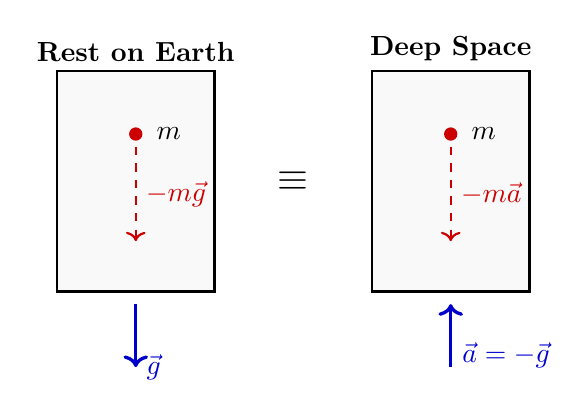
\begin{tikzpicture}[scale=0.8]
  % Left Box: Gravitational Field
  \draw[thick, fill=gray!5] (0,0) rectangle (2.5, 3.5);
  \node[above, font=\bfseries] at (1.25, 3.5) {Rest on Earth};
  \draw[->, very thick, blue!80!black] (1.25, -0.2) -- (1.25, -1.2) node[right] {$\vec{g}$};
  \fill[red!80!black] (1.25, 2.5) circle (3pt) node[right=4pt, text=black] {$m$};
  \draw[->, thick, dashed, red!80!black] (1.25, 2.3) -- (1.25, 0.8) node[midway, right] {$-m\vec{g}$};
  \draw[thick] (0.2, 0) -- (2.3, 0); % Floor emphasis

  % Right Box: Uniform Acceleration
  \begin{scope}[shift={(5,0)}]
    \draw[thick, fill=gray!5] (0,0) rectangle (2.5, 3.5);
    \node[above, font=\bfseries] at (1.25, 3.5) {Deep Space};
    \draw[->, very thick, blue!80!black] (1.25, -1.2) -- (1.25, -0.2) node[right=20pt, below=10pt] {$\vec{a} = -\vec{g}$};
    \fill[red!80!black] (1.25, 2.5) circle (3pt) node[right=4pt, text=black] {$m$};
    \draw[->, thick, dashed, red!80!black] (1.25, 2.3) -- (1.25, 0.8) node[midway, right] {$-m\vec{a}$};
    \draw[thick] (0.2, 0) -- (2.3, 0); % Floor emphasis
  \end{scope}

  % Equivalence symbol
  \node[font=\Large\bfseries] at (3.75, 1.75) {$\equiv$};
\end{tikzpicture}
\caption{The Einstein Equivalence Principle: indistinguishability between a uniform gravitational field (left) and a uniformly accelerated frame (right).}\
\label{fig:equivalence_principle}
\end{figure}


The Einstein Equivalence Principle (EEP) expands upon the WEP, declaring that no local non-gravitational experiment can distinguish a freely falling frame from a non-accelerating frame in flat spacetime. Locally, the laws of physics seamlessly reduce to those of special relativity. The Strong Equivalence Principle (SEP) further extends this indistinguishability to encompass all physical laws, including gravitational self-interaction.

\subsection*{From Equivalence to Geometry}
Because a uniform gravitational field can be "transformed away" by selecting a freely falling reference frame, gravity ceases to be a traditional force. Instead, freely falling particles trace out "straight lines" (geodesics) in a curved geometry. However, global inertial frames are physically unrealizable due to tidal forces—diverging or converging trajectories of test particles caused by a non-uniform gravitational field. Consequently, spacetime is modeled not as a globally flat Minkowski space, but as a differentiable manifold equipped with locally inertial frames at every point.

\begin{figure}[htbp]
\centering
\begin{minipage}{0.48\textwidth}
\centering
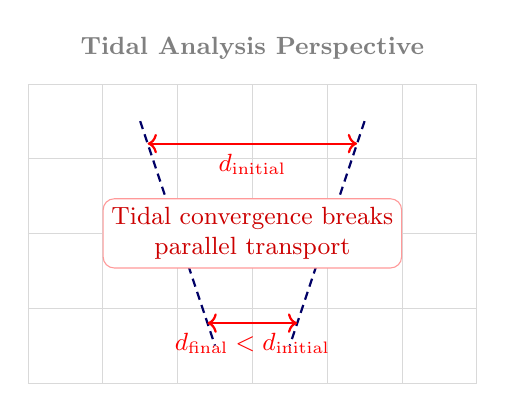
\begin{tikzpicture}[scale=0.95]
  % ----- Left Side: Tidal Analysis Grid -----
  % Rigid Cartesian Grid
  \draw[step=1cm, gray!30, very thin] (-3, 0) grid (3, 4);
  \node[gray, above, font=\bfseries\small] at (0, 4.2) {Tidal Analysis Perspective};

  % Falling paths (dashed trajectories)
  \draw[thick, blue!40!black, densely dashed] (-1.5, 3.5) -- (-0.5, 0.5);
  \draw[thick, blue!40!black, densely dashed] (1.5, 3.5) -- (0.5, 0.5);

  % Tidal effect annotations
  \draw[<->, thick, red] (-1.4, 3.2) -- (1.4, 3.2) node[midway, below, font=\small] {$d_{\text{initial}}$};
  \draw[<->, thick, red] (-0.6, 0.8) -- (0.6, 0.8) node[midway, below, font=\small] {$d_{\text{final}} < d_{\text{initial}}$};
  
  \node[fill=white, inner sep=3pt, draw=red!40, rounded corners, align=center, text=red!80!black, font=\small] at (0, 2) {Tidal convergence breaks \\ parallel transport};
\end{tikzpicture}
\end{minipage}
\hfill
\begin{minipage}{0.48\textwidth}
\centering
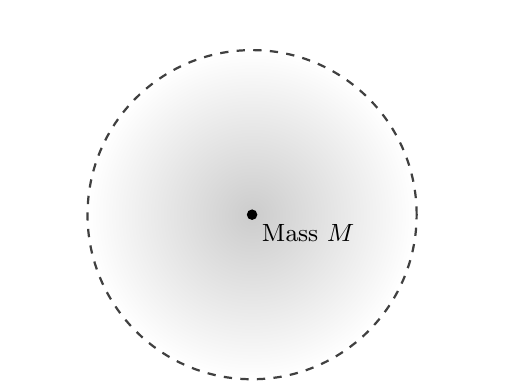
\begin{tikzpicture}[scale=0.95]
  % ----- Right Side: Gravitational Source Circle -----
  % Invisible bounding box matching the height of the left grid to maintain perfect baseline alignment
  \useasboundingbox (-3, 0) rectangle (3, 4.5);
  
  % Centered Gravitational Source (shifted vertically to center elegantly next to the grid)
  \begin{scope}[shift={(0, 2)}]
    \shade[inner color=gray!40, outer color=white] (0, 0) circle (2.2);
    \draw[thick, dashed, darkgray] (0, 0) circle (2.2);
    \fill (0, 0) circle (2pt) node[below right, font=\small] {Mass $M$};
  \end{scope}
\end{tikzpicture}
\end{minipage}
\caption{Geodesic deviation and tidal forces: spacetime curvature around mass $M$ causes initially parallel worldlines to converge.}
\label{fig:geodesic_deviation}
\end{figure}


\subsection*{Prediction: Gravitational Redshift}
An immediate, physically measurable consequence of the equivalence principle is the gravitational redshift of light. By modeling a uniform gravitational field as a constantly accelerating reference frame in flat spacetime, we can analyze a photon emitted from the base of a tower and received at the top. 

Applying the relativistic Doppler shift formula alongside standard kinematic relations for constant acceleration, the change in the photon's velocity relative to the accelerating frame over its flight time yields a fractional shift in wavelength. In the weak-field limit, this shift is directly proportional to the difference in the Newtonian gravitational potential $\Delta \Phi$:
\begin{equation} \frac{\Delta \lambda}{\lambda_0} \approx \frac{\Delta v}{c} = \frac{a_g z}{c^2} \end{equation}
\begin{equation} \frac{\Delta \lambda}{\lambda_0} \approx \Delta \Phi \end{equation}

\begin{figure}[htbp]
\centering
\begin{minipage}{0.48\textwidth}
\centering
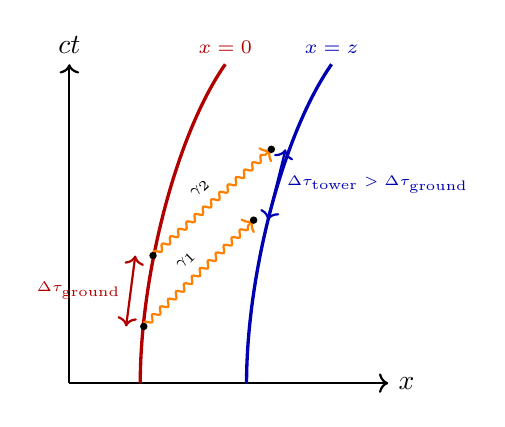
\begin{tikzpicture}[scale=0.9]
  % ----- Left Side: Spacetime Diagram -----
  % Axes
  \draw[->, thick] (0,0) -- (0, 4.5) node[above] {$ct$};
  \draw[->, thick] (0,0) -- (4.5, 0) node[right] {$x$};

  % Worldlines (Rindler-like curving)
  \draw[very thick, red!70!black] (1, 0) .. controls (1, 1.5) and (1.5, 3.5) .. (2.2, 4.5) 
    node[above, font=\scriptsize] {$x=0$};
  \draw[very thick, blue!70!black] (2.5, 0) .. controls (2.5, 1.5) and (3.0, 3.5) .. (3.7, 4.5) 
    node[above, font=\scriptsize] {$x=z$};

  % Photon 1
  \coordinate (E1) at (1.05, 0.8);
  \coordinate (R1) at (2.6, 2.3);
  \draw[->, thick, orange, decorate, decoration={snake, amplitude=1pt, segment length=4pt, post length=2pt}] 
    (E1) -- (R1) node[midway, sloped, above=1pt, text=black, font=\tiny] {$\gamma_1$};
  \fill (E1) circle (1.5pt); \fill (R1) circle (1.5pt);

  % Photon 2
  \coordinate (E2) at (1.18, 1.8);
  \coordinate (R2) at (2.85, 3.3);
  \draw[->, thick, orange, decorate, decoration={snake, amplitude=1pt, segment length=4pt, post length=2pt}] 
    (E2) -- (R2) node[midway, sloped, above=1pt, text=black, font=\tiny] {$\gamma_2$};
  \fill (E2) circle (1.5pt); \fill (R2) circle (1.5pt);

  % Time intervals
  \draw[<->, thick, red!70!black] (0.8, 0.8) -- (0.93, 1.8) 
    node[midway, left, font=\tiny] {$\Delta \tau_{\text{ground}}$};
  \draw[<->, thick, blue!70!black] (2.8, 2.3) -- (3.05, 3.3) 
    node[midway, right, font=\tiny] {$\Delta \tau_{\text{tower}} > \Delta \tau_{\text{ground}}$};
\end{tikzpicture}
\end{minipage}
\hfill
\begin{minipage}{0.48\textwidth}
\centering
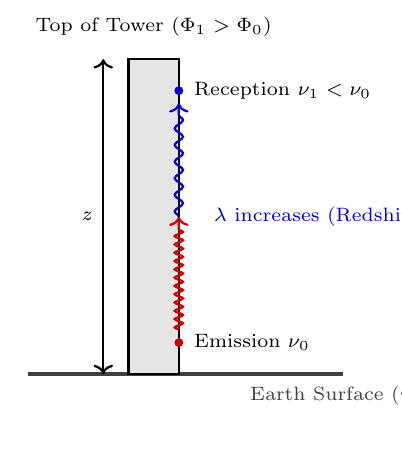
\begin{tikzpicture}[scale=0.8]
  % ----- Right Side: Physical Tower Diagram -----
  % Establish matching vertical bounds to ensure perfect alignment
  \useasboundingbox (-2, -0.8) rectangle (3.5, 5.5);

  % Ground Surface
  \draw[ultra thick, darkgray] (-2,0) -- (3,0) node[below, font=\scriptsize] {Earth Surface ($\Phi_0$)};
  
  % Tower
  \draw[thick, fill=gray!20] (-0.4, 0) rectangle (0.4, 5);
  \draw[<->, thick] (-0.8, 0) -- (-0.8, 5) node[midway, left, font=\scriptsize] {$z$};
  \node[above, font=\scriptsize] at (0, 5.2) {Top of Tower ($\Phi_1 > \Phi_0$)};

  % Photon Emission (Bottom)
  \fill[red!80!black] (0.4, 0.5) circle (2pt) node[right=2pt, text=black, font=\scriptsize] {Emission $\nu_0$};
  
  % Photon Reception (Top)
  \fill[blue!80!black] (0.4, 4.5) circle (2pt) node[right=2pt, text=black, font=\scriptsize] {Reception $\nu_1 < \nu_0$};

  % Wavelength stretch visualization
  \draw[->, thick, decorate, decoration={snake, amplitude=1.5pt, segment length=3pt, post length=4pt}, red!80!black] 
    (0.4, 0.7) -- (0.4, 2.5);
  \draw[->, thick, decorate, decoration={snake, amplitude=1.5pt, segment length=6pt, post length=4pt}, blue!80!black] 
    (0.4, 2.5) -- (0.4, 4.3);
    
  \node[right, font=\scriptsize, text=blue!80!black] at (0.8, 2.5) {$\lambda$ increases (Redshift)};
\end{tikzpicture}
\end{minipage}
\caption{Gravitational redshift and time dilation: spacetime diagram of metric variation (left) and physical schematic of wavelength increase (right).}
\label{fig:gravitational_redshift}
\end{figure}

\section{What Is a Manifold?}
A differentiable manifold $\mathcal{M}$ of dimension $n$ is a continuous topological space that, at a sufficiently microscopic scale, is indistinguishable from Euclidean space $\mathbb{R}^n$. Common examples in topology and physics include $\mathbb{R}^n$ itself, the $n$-sphere $S^n$, the $n$-torus $T^n$, and continuous Lie Groups. 

\subsection*{Formal Definition and Coordinate Charts}
The rigorous definition of a manifold relies on the construction of an \emph{atlas}, which is a collection of compatible coordinate \emph{charts}. Each chart consists of an open subset of the manifold mapped bijectively to an open subset of $\mathbb{R}^n$.

\begin{figure}[htbp]
\centering
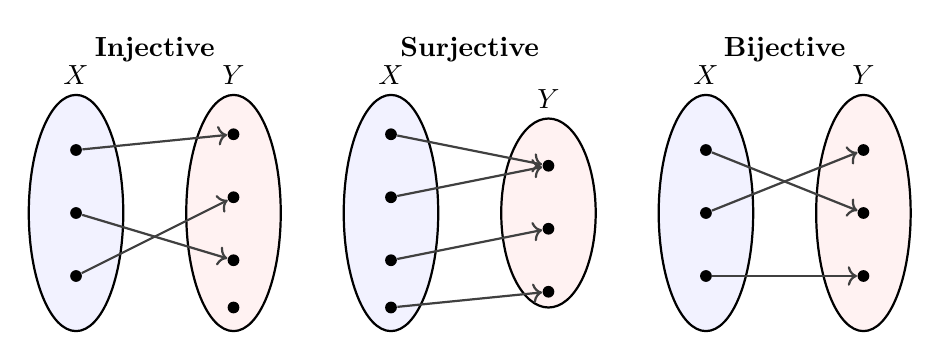
\begin{tikzpicture}[scale=1]
  \tikzset{dot/.style={circle, fill=black, inner sep=1.5pt}}
  
  % Injective
  \begin{scope}[shift={(0,0)}]
    \node[above, font=\bfseries] at (1, 2.8) {Injective};
    \draw[thick, fill=blue!5] (0, 1) ellipse (0.6 and 1.5) node[above=1.5cm] {$X$};
    \draw[thick, fill=red!5] (2, 1) ellipse (0.6 and 1.5) node[above=1.5cm] {$Y$};
    \node[dot] (a1) at (0, 1.8) {}; \node[dot] (a2) at (0, 1) {}; \node[dot] (a3) at (0, 0.2) {};
    \node[dot] (b1) at (2, 2) {}; \node[dot] (b2) at (2, 1.2) {}; \node[dot] (b3) at (2, 0.4) {}; \node[dot] (b4) at (2, -0.2) {};
    \draw[->, thick, darkgray] (a1) -- (b1); 
    \draw[->, thick, darkgray] (a2) -- (b3); 
    \draw[->, thick, darkgray] (a3) -- (b2);
  \end{scope}

  % Surjective
  \begin{scope}[shift={(4,0)}]
    \node[above, font=\bfseries] at (1, 2.8) {Surjective};
    \draw[thick, fill=blue!5] (0, 1) ellipse (0.6 and 1.5) node[above=1.5cm] {$X$};
    \draw[thick, fill=red!5] (2, 1) ellipse (0.6 and 1.2) node[above=1.2cm] {$Y$};
    \node[dot] (c1) at (0, 2) {}; \node[dot] (c2) at (0, 1.2) {}; \node[dot] (c3) at (0, 0.4) {}; \node[dot] (c4) at (0, -0.2) {};
    \node[dot] (d1) at (2, 1.6) {}; \node[dot] (d2) at (2, 0.8) {}; \node[dot] (d3) at (2, 0) {};
    \draw[->, thick, darkgray] (c1) -- (d1); 
    \draw[->, thick, darkgray] (c2) -- (d1); 
    \draw[->, thick, darkgray] (c3) -- (d2); 
    \draw[->, thick, darkgray] (c4) -- (d3);
  \end{scope}

  % Bijective
  \begin{scope}[shift={(8,0)}]
    \node[above, font=\bfseries] at (1, 2.8) {Bijective};
    \draw[thick, fill=blue!5] (0, 1) ellipse (0.6 and 1.5) node[above=1.5cm] {$X$};
    \draw[thick, fill=red!5] (2, 1) ellipse (0.6 and 1.5) node[above=1.5cm] {$Y$};
    \node[dot] (e1) at (0, 1.8) {}; \node[dot] (e2) at (0, 1) {}; \node[dot] (e3) at (0, 0.2) {};
    \node[dot] (f1) at (2, 1.8) {}; \node[dot] (f2) at (2, 1) {}; \node[dot] (f3) at (2, 0.2) {};
    \draw[->, thick, darkgray] (e1) -- (f2); 
    \draw[->, thick, darkgray] (e2) -- (f1); 
    \draw[->, thick, darkgray] (e3) -- (f3);
  \end{scope}
\end{tikzpicture}
\caption{Classification of injective, surjective, and bijective mappings between sets $X$ and $Y$.}
\label{fig:mapping_types}
\end{figure}
\begin{figure}[htbp]
\centering
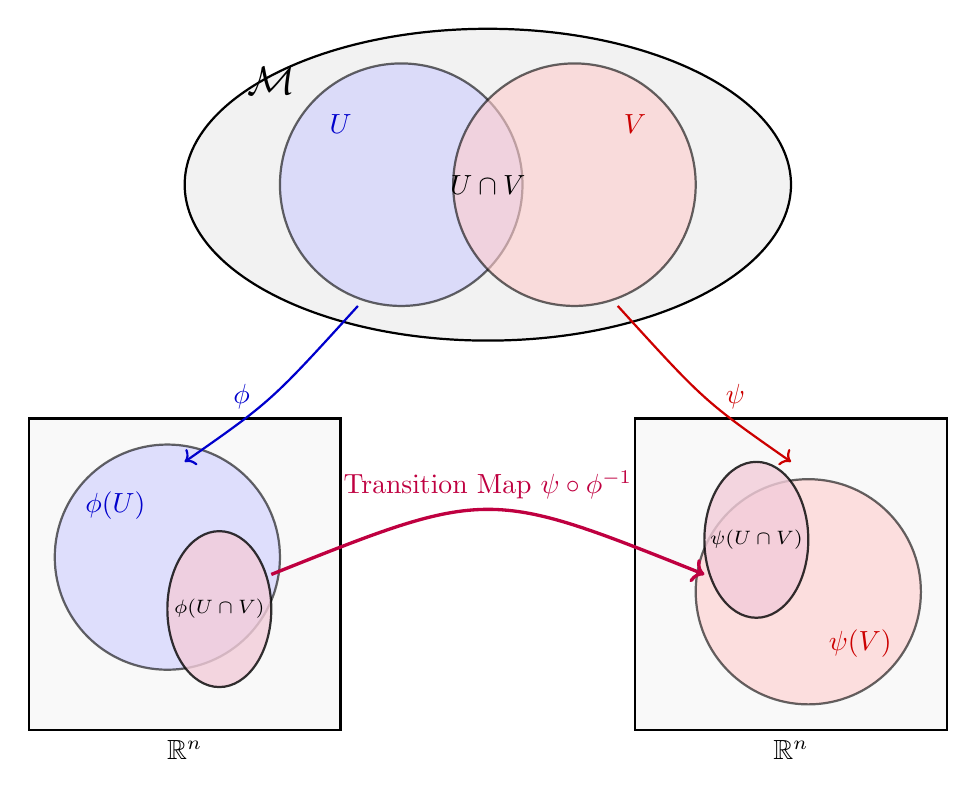
\begin{tikzpicture}[scale=1.1]
  % Manifold M
  \draw[thick, fill=gray!10] (0,0) ellipse (3.5 and 1.8);
  \node[font=\Large\bfseries] at (-2.5, 1.2) {$\mathcal{M}$};
  
  % Sets U and V
  \draw[thick, fill=blue!20, opacity=0.6] (-1, 0) circle (1.4);
  \node[blue!80!black, font=\bfseries] at (-1.7, 0.7) {$U$};
  
  \draw[thick, fill=red!20, opacity=0.6] (1, 0) circle (1.4);
  \node[red!80!black, font=\bfseries] at (1.7, 0.7) {$V$};
  
  % U intersect V (Manifold)
  \node[font=\bfseries] at (0, 0) {$U \cap V$};
  
  % Chart 1 (Left) - R^n space
  \begin{scope}[shift={(-3.5, -4.5)}]
    \draw[thick, fill=gray!5] (-1.8, -1.8) rectangle (1.8, 1.8);
    \node[below] at (0, -1.8) {$\mathbb{R}^n$};
    \draw[thick, fill=blue!20, opacity=0.6] (-0.2,0.2) circle (1.3);
    \node[blue!80!black] at (-0.8, 0.8) {$\phi(U)$};
    % Image of intersection
    \draw[thick, fill=purple!20, opacity=0.8] (0.4,-0.4) ellipse (0.6 and 0.9);
    \node[font=\scriptsize, align=center] at (0.4, -0.4) {$\phi(U \cap V)$};
  \end{scope}

  % Chart 2 (Right) - R^n space
  \begin{scope}[shift={(3.5, -4.5)}]
    \draw[thick, fill=gray!5] (-1.8, -1.8) rectangle (1.8, 1.8);
    \node[below] at (0, -1.8) {$\mathbb{R}^n$};
    \draw[thick, fill=red!20, opacity=0.6] (0.2,-0.2) circle (1.3);
    \node[red!80!black] at (0.8, -0.8) {$\psi(V)$};
    % Image of intersection
    \draw[thick, fill=purple!20, opacity=0.8] (-0.4,0.4) ellipse (0.6 and 0.9);
    \node[font=\scriptsize, align=center] at (-0.4, 0.4) {$\psi(U \cap V)$};
  \end{scope}
  
  % Mappings from Manifold to R^n
  \draw[->, thick, blue!80!black] (-1.5, -1.4) .. controls (-2.5, -2.5) .. (-3.5, -3.2) node[midway, left=4pt] {$\phi$};
  \draw[->, thick, red!80!black] (1.5, -1.4) .. controls (2.5, -2.5) .. (3.5, -3.2) node[midway, right=4pt] {$\psi$};
  
  % Transition Map between R^n charts
  \draw[->, very thick, purple] (-2.5, -4.5) .. controls (0, -3.5) .. (2.5, -4.5) node[midway, above] {Transition Map $\psi \circ \phi^{-1}$};
\end{tikzpicture}
\caption{Atlas construction on a manifold $\mathcal{M}$: local coordinate charts $\phi$ and $\psi$ linked by a smooth transition map $\psi \circ \phi^{-1}$.}
\label{fig:transition_map}
\end{figure}
Where two charts overlap on the manifold, the map detailing the coordinate transformation between the two representations in $\mathbb{R}^n$ must be smooth ($C^\infty$). This requirement guarantees that the differential structure of the manifold is globally well-defined and invariant under arbitrary coordinate choices.



\subsubsection*{Stereographic Projection on $S^2$}
A canonical example of manifold charting is the stereographic projection of the 2-sphere, defined by the locus $(x^1)^2 + (x^2)^2 + (x^3)^2 = 1$. Because a sphere cannot be mapped bijectively to a plane globally without encountering a singularity, at least two overlapping charts are required to form a complete atlas.

\begin{figure}[htbp]
\centering
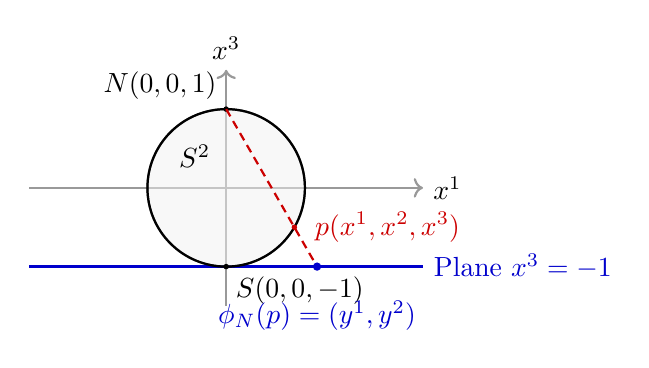
\begin{tikzpicture}[scale=1.0]
  % Axes
  \draw[->, thick, gray!80] (-2.5, 0) -- (2.5, 0) node[right, text=black] {$x^1$};
  \draw[->, thick, gray!80] (0, -1.5) -- (0, 1.5) node[above, text=black] {$x^3$};

  % Projection Plane x^3 = -1
  \draw[very thick, blue!80!black] (-2.5, -1) -- (2.5, -1) node[right] {Plane $x^3 = -1$};

  % Sphere S^2 cross-section (S^1)
  \draw[thick, fill=gray!10, opacity=0.5] (0,0) circle (1);
  \draw[thick] (0,0) circle (1);
  \node at (-0.4, 0.4) {$S^2$};
  
  % Poles
  \fill[black] (0, 1) circle (1pt) node[above left] {$N (0,0,1)$};
  \fill[black] (0, -1) circle (1pt) node[below right] {$S (0,0,-1)$};

  % Point P on the sphere (picking an arbitrary point)
  \coordinate (P) at (0.866, -0.5); % (sin(60), -cos(60))
  \fill[red!80!black] (P) circle (1pt) node[right=4pt] {$p (x^1, x^2, x^3)$};

  % Projection line from N through P to the plane
  % The line intersects z=-1 at x = 2/sqrt(3) ≈ 1.154
  \coordinate (Proj) at (1.154, -1);
  \draw[thick, densely dashed, red!80!black] (0,1) -- (Proj);
  
  % Projected point on the plane
  \fill[blue!80!black] (Proj) circle (1.5pt) node[below=9pt] {$\phi_N(p) = (y^1, y^2)$};
\end{tikzpicture}
\caption{Stereographic projection of the 2-sphere ($S^2$) from the North pole onto the South pole tangent plane, mapping $S^2 \setminus \{N\}$.}
\label{fig:stereographic_projection}
\end{figure}


The primary chart projects from the North Pole ($N$) onto the tangent plane at the South Pole, uniquely mapping every point except $N$ itself:
\begin{equation} (y^1, y^2) = \phi_N(x^1, x^2, x^3) = \left( \frac{2x^1}{1-x^3}, \frac{2x^2}{1-x^3} \right) \end{equation}
Conversely, the secondary chart covers the sphere excluding the South Pole ($S$), projecting onto the tangent plane at the North Pole:
\begin{equation} (z^1, z^2) = \phi_S(x^1, x^2, x^3) = \left( \frac{2x^1}{1+x^3}, \frac{2x^2}{1+x^3} \right) \end{equation}

To rigorously define the differential structure in the region where these charts overlap (the sphere excluding both poles), we compute the transition map $\phi_S \circ \phi_N^{-1}$. By analytically inverting $\phi_N$ and substituting the resulting Euclidean coordinates into $\phi_S$, the coordinate transformation equations are established:
\begin{equation} z^1 = \frac{4y^1}{(y^1)^2 + (y^2)^2}, \quad z^2 = \frac{4y^2}{(y^1)^2 + (y^2)^2} \end{equation}
This transition map is manifestly $C^\infty$ everywhere in the overlap region, cementing $S^2$ as a smooth manifold.

\subsection*{The Chain Rule}
The formalism of calculus on manifolds heavily utilizes the multivariable chain rule, operating smoothly across sequential mappings and chart transformations.

% Drawing 1: Composition of mappings between spaces (Manifolds)
\begin{figure}[htbp]
\centering
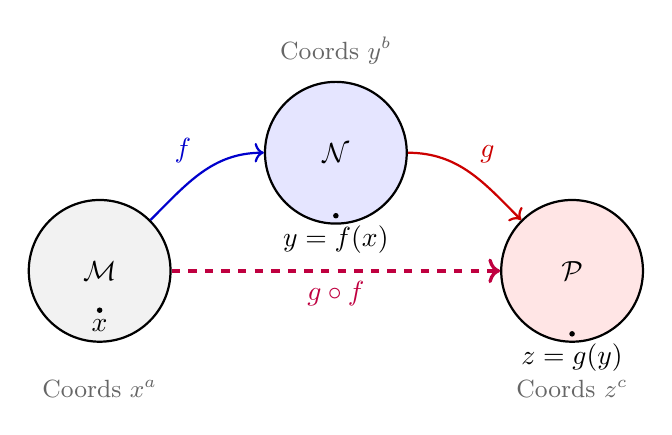
\begin{tikzpicture}[scale=1.0]
  % Spaces
  \node (M) at (0,0) [circle, draw, thick, fill=gray!10, minimum size=1.8cm] {$\mathcal{M}$};
  \node (N) at (3,1.5) [circle, draw, thick, fill=blue!10, minimum size=1.8cm] {$\mathcal{N}$};
  \node (P) at (6,0) [circle, draw, thick, fill=red!10, minimum size=1.8cm] {$\mathcal{P}$};

  % Mappings
  \draw[->, thick, blue!80!black] (M) to[out=45, in=180] node[midway, above left] {$f$} (N);
  \draw[->, thick, red!80!black] (N) to[out=0, in=135] node[midway, above right] {$g$} (P);
  \draw[->, very thick, dashed, purple] (M) to[out=0, in=180] node[midway, below] {$g \circ f$} (P);
  
  % Points and Coordinates
  \fill[black] (0.0, -0.5) circle (1pt) node[below] {$x$};
  \fill[black] (3, 0.7) circle (1pt) node[below] {$y = f(x)$};
  \fill[black] (6.0, -0.8) circle (1pt) node[below] {$z = g(y)$};
  
  % Coordinate system labels
  \node[font=\small, text=gray!80!black] at (0, -1.5) {Coords $x^a$};
  \node[font=\small, text=gray!80!black] at (3, 2.8) {Coords $y^b$};
  \node[font=\small, text=gray!80!black] at (6, -1.5) {Coords $z^c$};
\end{tikzpicture}
\caption{Composition of smooth maps between manifolds.}
\label{fig:map_composition}
\end{figure}


Applying the chain rule explicitly to coordinate partial derivatives ensures that scalar and vector expressions remain functionally covariant across spaces:
\begin{equation} \frac{\partial (g \circ f)^c}{\partial x^a} = \sum_{b=1}^n \frac{\partial f^b}{\partial x^a} \frac{\partial g^c}{\partial y^b} \end{equation}
\begin{equation} \frac{\partial}{\partial x^a} = \sum_{b=1}^n \frac{\partial y^b}{\partial x^a} \frac{\partial}{\partial y^b} \end{equation}

\section{Vectors Again}
In differential geometry, intuitive Euclidean vectors are entirely replaced by directional derivatives. A tangent vector $X$ residing in the tangent space $T_p$ at a point $p$ is strictly defined as a linear operator that maps smooth functions to real numbers, rigorously satisfying both linearity and the Leibniz (product) rule:
\begin{equation} X(fg) = f (X(g)) + g (X(f)) \end{equation}

\subsection*{The Coordinate Basis}
For any given coordinate chart $x^\mu$, the corresponding set of partial derivative operators $\{\partial_\mu\}$ constitutes a natural, complete basis for the tangent space at any covered point.


% Drawing 2: Curved surface with coordinate lines and tangent basis
\begin{figure}[htbp]
\centering
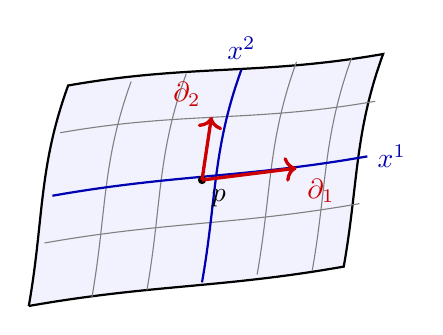
\begin{tikzpicture}[scale=1.0]
  % Define point p
  \coordinate (P) at (2.2, 1.6);

  % Curved surface
  \draw[thick, fill=blue!5] (0,0) to[out=10, in=190] (4,0.5) 
        to[out=80, in=250] (4.5,3.2) 
        to[out=190, in=10] (0.5,2.8) 
        to[out=250, in=80] (0,0);
        
  % Coordinate lines (thin gray)
  \draw[gray, thin] (0.8, 0.1) to[out=80, in=250] (1.3, 2.85);
  \draw[gray, thin] (1.5, 0.2) to[out=80, in=250] (2.0, 2.95);
  \draw[gray, thin] (2.9, 0.4) to[out=80, in=250] (3.4, 3.1);
  \draw[gray, thin] (3.6, 0.45) to[out=80, in=250] (4.1, 3.15);

  \draw[gray, thin] (0.2, 0.8) to[out=10, in=190] (4.2, 1.3);
  \draw[gray, thin] (0.4, 2.2) to[out=10, in=190] (4.4, 2.6);

  % Highlighted coordinate lines passing through p
  % x^1 curve
  \draw[blue!70!black, thick] (0.3, 1.4) to[out=10, in=190] (4.3, 1.9) node[right] {$x^1$};
  % x^2 curve
  \draw[blue!70!black, thick] (2.2, 0.3) to[out=80, in=250] (2.7, 3.0) node[above] {$x^2$};

  % Mark point p
  \fill[black] (P) circle (1.5pt) node[below right] {$p$};

  % Tangent basis vectors
  \draw[->, very thick, red!80!black] (P) -- ++(1.2, 0.15) node[below right] {$\partial_1$};
  \draw[->, very thick, red!80!black] (P) -- ++(0.12, 0.8) node[above left] {$\partial_2$};

\end{tikzpicture}
\caption{Coordinate curves and their tangent basis vectors at a point $p$.}
\label{fig:tangent_basis}
\end{figure}

Applying the multivariable chain rule to a function parameterized by a curve $\lambda$ natively extracts the vector components $dx^\mu/d\lambda$ paired directly with the basis vectors:
\begin{equation} \frac{d}{d\lambda} = \frac{dx^\mu}{d\lambda} \partial_\mu \end{equation}

\subsection*{Transformation Properties}
Under an arbitrary coordinate transformation from $x^\mu$ to $x^{\mu'}$, the basis vectors transform covariantly according to the partial derivatives of the coordinate maps:
\begin{equation} \partial_{\mu'} = \frac{\partial x^\mu}{\partial x^{\mu'}} \partial_\mu \end{equation}
Conversely, to ensure the geometric vector remains invariant as an absolute physical entity, its numerical components must transform contravariantly:
\begin{equation} V^{\mu'} = \frac{\partial x^{\mu'}}{\partial x^\mu} V^\mu \end{equation}

% Drawing 3: Curved surface patch with two overlapping coordinate grids
\begin{figure}[htbp]
\centering
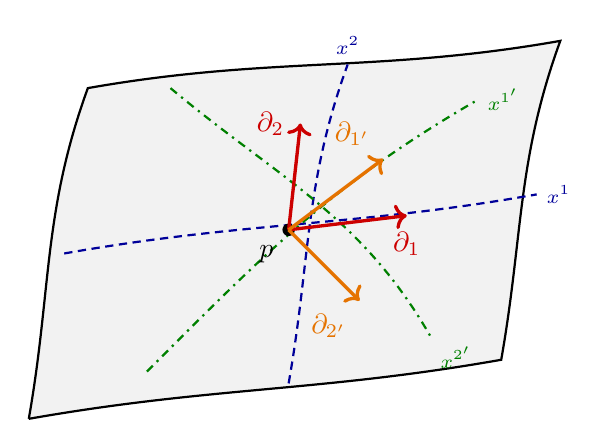
\begin{tikzpicture}[scale=1.5]
  % Define point p
  \coordinate (P) at (2.2, 1.6);

  % Curved surface patch
  \draw[thick, fill=gray!10] (0,0) to[out=10, in=190] (4,0.5) 
        to[out=80, in=250] (4.5,3.2) 
        to[out=190, in=10] (0.5,2.8) 
        to[out=250, in=80] (0,0);

  % Grid 1 (x^\mu) lines
  \draw[blue!60!black, thick, densely dashed] (0.3, 1.4) to[out=10, in=190] (4.3, 1.9) node[right, font=\scriptsize] {$x^1$};
  \draw[blue!60!black, thick, densely dashed] (2.2, 0.3) to[out=80, in=250] (2.7, 3.0) node[above, font=\scriptsize] {$x^2$};

  % Grid 2 (x^{\mu'}) lines
  \draw[green!50!black, thick, dash dot] (1.0, 0.4) to[out=45, in=210] (3.8, 2.7) node[right, font=\scriptsize] {$x^{1'}$};
  \draw[green!50!black, thick, dash dot] (1.2, 2.8) to[out=-40, in=120] (3.4, 0.7) node[below right, font=\scriptsize] {$x^{2'}$};

  % Mark point p
  \fill[black] (P) circle (1.5pt) node[below left=2pt] {$p$};

  % Basis Vectors for Grid 1 (Red)
  \draw[->, very thick, red!80!black] (P) -- ++(1.0, 0.12) node[below=2pt] {$\partial_1$};
  \draw[->, very thick, red!80!black] (P) -- ++(0.1, 0.9) node[left=2pt] {$\partial_2$};

  % Basis Vectors for Grid 2 (Orange)
  \draw[->, very thick, orange!90!black] (P) -- ++(0.8, 0.6) node[above left=1pt] {$\partial_{1'}$};
  \draw[->, very thick, orange!90!black] (P) -- ++(0.6, -0.6) node[below left=1pt] {$\partial_{2'}$};

\end{tikzpicture}
\caption{Transformation of basis vectors under a local coordinate change.}
\label{fig:coordinate_transformation}
\end{figure}

\subsection*{The Commutator (Lie Bracket)}
The commutator of two vector fields natively generates a third, completely independent vector field, quantifying the failure of the corresponding directional derivatives to commute. The coordinate representation is computed by directly expanding the action of the operators on a generic scalar function:
\begin{equation} [X, Y](f) \equiv X(Y(f)) - Y(X(f)) \end{equation}
\begin{equation} [X, Y]^\nu = X^\lambda \partial_\lambda Y^\nu - Y^\lambda \partial_\lambda X^\nu \end{equation}

\section{Tensors Again}
\subsection*{Dual Vectors (One-Forms)}
The cotangent space $T_p^*$ represents the algebraic dual to the tangent space, containing one-forms (dual vectors) designed to map vectors linearly into the field of real numbers. The formal action of the gradient $df$ on a tangent vector yields the rate of change of the function along the corresponding curve:
\begin{equation} df\left(\frac{d}{d\lambda}\right) = \frac{df}{d\lambda} \end{equation}

\subsection*{Basis and Components}
The coordinate differentials $\{dx^\mu\}$ natively establish the basis for the cotangent space. Their action on the tangent basis is defined via the Kronecker delta, enforcing strict duality:
\begin{equation} dx^\mu (\partial_\nu) \equiv \partial_\nu (x^\mu) = \frac{\partial x^\mu}{\partial x^\nu} = \delta^\mu_\nu \end{equation}
Following this structure, the components of a dual vector $\omega_\mu$ necessarily undergo covariant transformation to preserve scalar invariance:
\begin{equation} \omega_{\nu'} = \frac{\partial x^\mu}{\partial x^{\nu'}} \omega_\mu \end{equation}

\subsection*{General Tensors}
A general tensor of type $(k,l)$ constitutes a multilinear mapping over $k$ dual vectors and $l$ vectors. Its formal expansion relies on the tensor product $\otimes$ of the underlying basis structures:
\begin{equation} T = {T^{\mu_1 \dots \mu_k}}_{\nu_1 \dots \nu_l} \partial_{\mu_1} \otimes \dots \otimes \partial_{\mu_k} \otimes dx^{\nu_1} \otimes \dots \otimes dx^{\nu_l} \end{equation}
The numerical components are dynamically updated under a coordinate transformation via an explicit chain-rule multiplication for every index:
\begin{equation} {T^{\mu'_1 \dots \mu'_k}}_{\nu'_1 \dots \nu'_l} = \frac{\partial x^{\mu'_1}}{\partial x^{\mu_1}} \dots \frac{\partial x^{\nu_1}}{\partial x^{\nu'_1}} \dots {T^{\mu_1 \dots \mu_k}}_{\nu_1 \dots \nu_l} \end{equation}

\subsection*{Example: Transforming a (0,2) Tensor}
Consider the application of the general tensorial transformation law to a covariant rank-2 tensor $S = S_{\mu\nu} dx^\mu dx^\nu = (dx)^2 + x^2 (dy)^2$ under the non-linear transformation substitution $x' = 2x/y$ and $y' = y/2$. Applying the Jacobian transformation directly to the differentials yields the updated metric components:
\begin{equation} \label{S_transform} S_{\mu'\nu'} = \begin{pmatrix} (y')^2 & x'y' \\ x'y' & (x')^2 + 4(x'y')^2 \end{pmatrix} \end{equation}

\subsection*{The Failure of Partial Derivatives}
While tensors inherently preserve their geometric structure under coordinate maps, the partial derivative of a vector component $\partial_\mu W_\nu$ intrinsically fails to transform as a valid tensor. Applying the coordinate transformation law directly exposes the existence of anomalous, non-tensorial second derivatives:
\begin{equation} \partial_{\mu'} W_{\nu'} = \frac{\partial x^\mu}{\partial x^{\mu'}} \frac{\partial x^\nu}{\partial x^{\nu'}} (\partial_\mu W_\nu) + W_\nu \frac{\partial^2 x^\nu}{\partial x^{\mu'} \partial x^{\nu'}} \end{equation}
The presence of the second term guarantees that partial derivatives are dependent on the specific coordinate choice except under strictly linear affine transformations. This profound inadequacy mathematically necessitates the introduction of the \textbf{covariant derivative} and connection coefficients.

\section{The Metric}
The foundational pillar characterizing a specific manifold geometry is the metric tensor $g_{\mu\nu}$, a symmetric, nondegenerate (0,2) tensor that defines intrinsic distances, angles, and causal structure, enabling the construction of the invariant line element:
\begin{equation} g^{\mu\nu} g_{\nu\sigma} = \delta^\mu_\sigma \end{equation}
\begin{equation} ds^2 = g_{\mu\nu} dx^\mu dx^\nu \end{equation}

\subsection*{Example: Flat Space in Spherical Coordinates}
Transforming the familiar flat space Euclidean line element into standard spherical coordinates necessitates substituting the Cartesian differentials derived from standard trigonometric projections. Doing so dynamically recovers the characteristic diagonal metric form:
\begin{equation} ds^2 = dr^2 + r^2 d\theta^2 + r^2\sin^2\theta d\phi^2 \end{equation}
By enforcing a constant radius ($r=R$, $dr=0$), the induced metric upon the geometry of the 2-sphere $S^2$ is flawlessly isolated:
\begin{equation} ds^2 = R^2 d\theta^2 + R^2\sin^2\theta d\phi^2 \end{equation}



% Drawing 4: Infinitesimal triangle on a 2-sphere patch
\begin{figure}[htbp]
\centering
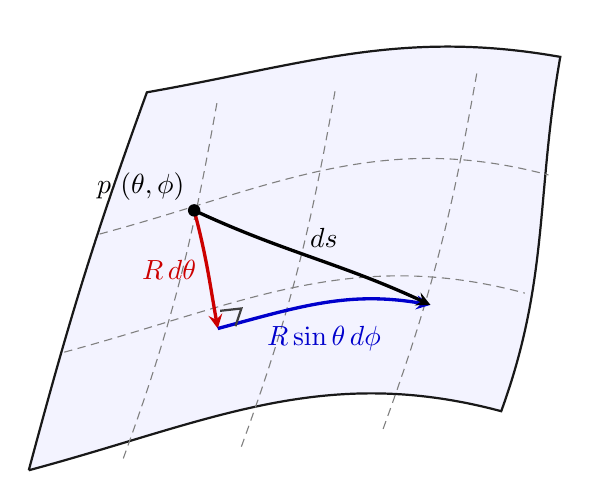
\begin{tikzpicture}[scale=1.5]
  % Draw a curved patch of the 2-sphere
  \draw[thick, fill=blue!5, opacity=0.9] (0,0) to[out=15, in=165] (4,0.5) 
        to[out=70, in=260] (4.5, 3.5) 
        to[out=170, in=10] (1, 3.2) 
        to[out=250, in=75] (0,0);
        
  % Grid lines (Lines of constant theta and phi) to imply curvature
  \draw[gray, thin, densely dashed] (0.8, 0.1) to[out=70, in=260] (1.6, 3.15);
  \draw[gray, thin, densely dashed] (1.8, 0.2) to[out=70, in=260] (2.6, 3.25);
  \draw[gray, thin, densely dashed] (3.0, 0.35) to[out=70, in=260] (3.8, 3.4);
  
  \draw[gray, thin, densely dashed] (0.3, 1.0) to[out=15, in=165] (4.2, 1.5);
  \draw[gray, thin, densely dashed] (0.6, 2.0) to[out=15, in=165] (4.4, 2.5);

  % Infinitesimal right-triangle points
  % A = Point p (theta, phi)
  % B = Point displaced by d\theta (theta + d\theta, phi)
  % C = Point displaced by d\theta and d\phi (theta + d\theta, phi + d\phi)
  \coordinate (A) at (1.4, 2.2);
  \coordinate (B) at (1.6, 1.2);
  \coordinate (C) at (3.4, 1.4);

  % d(theta) side (meridian - arc length R d\theta)
  \draw[very thick, red!80!black, -stealth] (A) to[out=285, in=100] (B);
  \node[left, red!80!black] at (1.5, 1.7) {$R \, d\theta$};

  % d(phi) side (parallel of latitude - arc length R \sin\theta d\phi)
  \draw[very thick, blue!80!black, -stealth] (B) to[out=15, in=170] (C);
  \node[below, blue!80!black] at (2.5, 1.3) {$R \sin\theta \, d\phi$};

  % ds side (hypotenuse - invariant interval)
  \draw[very thick, black, -stealth] (A) to[out=-25, in=155] (C);
  \node[above right, font=\bfseries] at (2.3, 1.8) {$ds$};

  % Mark the starting point
  \fill (A) circle (1.5pt) node[above left] {$p \ (\theta, \phi)$};

  % Fake right angle symbol (approximated for curved perspective)
  \draw[thick, darkgray] (1.75, 1.22) -- (1.8, 1.37) -- (1.62, 1.35);

\end{tikzpicture}
\caption{Infinitesimal line element $ds$ on the surface of a 2-sphere.}
\label{fig:sphere_line_element}
\end{figure}



\subsection*{Locally Inertial Coordinates (LIC)}
The Einstein Equivalence Principle mandates the existence of Locally Inertial Coordinates (LIC) $x^{\hat{\mu}}$ at any selected event $p$. Within this frame, the metric strictly mimics flat space, and gravitational forces strictly vanish to first order:
\begin{align} g_{\hat{\mu}\hat{\nu}}(p) &= \eta_{\hat{\mu}\hat{\nu}} \ \partial_{\hat{\sigma}} g_{\hat{\mu}\hat{\nu}}(p) &= 0 \end{align}
Comparing the coordinate degrees of freedom available in 4D against the symmetric components of the metric reveals that a second-order expansion lacks exactly 20 parameters. This rigorous geometric shortfall intrinsically defines the 20 independent components of the Riemann curvature tensor.

The true power of metric formulation rests in manifesting equations independent of the chosen reference frame. For instance, computing relative velocities via tensor contraction with the metric preserves coordinate invariance natively:
\begin{equation} v = \sqrt{1 - (g_{\mu\nu} U^\mu V^\nu)^{-2}} \end{equation}

\section{An Expanding Universe}
The dynamic spatial scaling of homogeneous and isotropic cosmologies is cleanly parameterized by the Robertson-Walker (RW) metric, where the scale factor $a(t)$ maps the expansion rate explicitly against proper cosmic time $t$:
\begin{equation}\label{eq:rw-metric} ds^2 = -dt^2 + a^2(t)[(dx)^2 + (dy)^2 + (dz)^2] \end{equation}
For idealized cosmological models parameterized geometrically by $a(t) = t^q$ (where $0 < q < 1$), the metric models decelerating expansions characteristic of matter or radiation dominated eras.

\subsection*{Light Cones and Particle Horizon}
The causal boundaries within the RW cosmology are distinctly delineated by tracking null photon paths ($ds^2 = 0$). By rigorously separating variables and integrating the null differential equation from the initial singularity $t=0$ to an arbitrary observation time $t$, the absolute comoving particle horizon is established:
\begin{equation} -\left(\frac{dt}{d\lambda}\right)^2 + t^{2q} \left(\frac{dx}{d\lambda}\right)^2 = 0 \implies \left(\frac{dx}{dt}\right)^2 = t^{-2q} \end{equation}
\begin{equation} x(t) = \pm \int_{t_0}^{t} (t')^{-q} dt' = \pm \frac{t^{1-q}}{1-q} \end{equation}


% Drawing 5: Big Bang singularity and cosmological particle horizon
\begin{figure}[htbp]
\centering
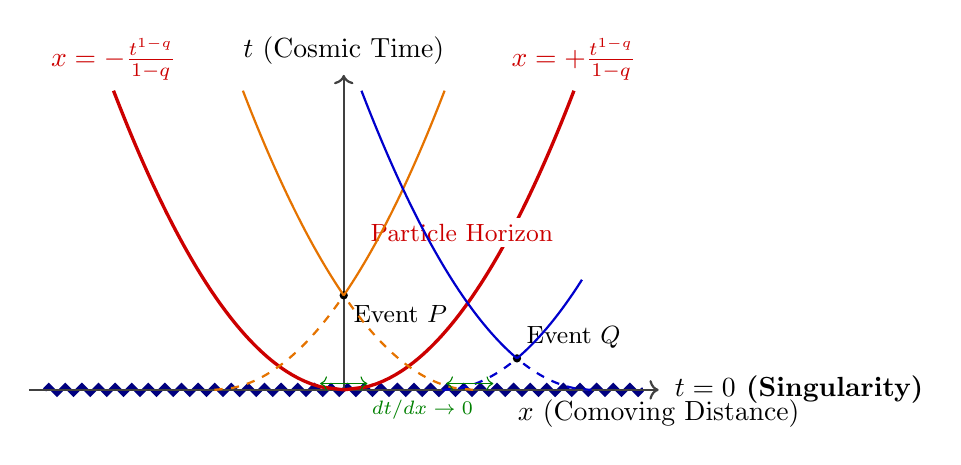
\begin{tikzpicture}[scale=1.0]
  % Singularity (Big Bang)
  \draw[ultra thick, decorate, decoration={zigzag, segment length=6pt, amplitude=1.5pt}, blue!50!black] 
    (-3.8, 0) -- (3.8, 0);
  \node[right=8pt, text=black, font=\bfseries] at (3.8, 0) {$t=0$ (Singularity)};

  % Axes
  \draw[->, thick, darkgray] (0, 0) -- (0, 4) node[above, text=black] {$t$ (Cosmic Time)};
  \draw[->, thick, darkgray] (-4, 0) -- (4, 0) node[below, text=black] {$x$ (Comoving Distance)};

  % Particle Horizon (Future light cone from origin)
  % Using a scale factor 1.5 for the x-coordinate to represent 1/(1-q)
  \draw[very thick, red!80!black, variable=\t, domain=0:3.8, samples=100] 
    plot ({1.5*sqrt(\t)}, {\t}) node[above] {$x = +\frac{t^{1-q}}{1-q}$};
  \draw[very thick, red!80!black, variable=\t, domain=0:3.8, samples=100] 
    plot ({-1.5*sqrt(\t)}, {\t}) node[above] {$x = -\frac{t^{1-q}}{1-q}$};
  \node[red!80!black, fill=white, inner sep=2pt, font=\small] at (1.5, 2.0) {Particle Horizon};

  % Event P and its light cone
  \fill (0, 1.2) circle (1.5pt) node[below right, font=\small] {Event $P$};
  
  % Future light cone of P
  \draw[thick, orange!90!black, variable=\t, domain=1.2:3.8, samples=100] 
    plot ({1.5*(sqrt(\t) - sqrt(1.2))}, {\t});
  \draw[thick, orange!90!black, variable=\t, domain=1.2:3.8, samples=100] 
    plot ({-1.5*(sqrt(\t) - sqrt(1.2))}, {\t});
    
  % Past light cone of P (arriving rays)
  \draw[thick, dashed, orange!90!black, variable=\t, domain=0:1.2, samples=50] 
    plot ({1.5*(sqrt(\t) - sqrt(1.2))}, {\t});
  \draw[thick, dashed, orange!90!black, variable=\t, domain=0:1.2, samples=50] 
    plot ({-1.5*(sqrt(\t) - sqrt(1.2))}, {\t});

  % Event Q and its light cone (off-center)
  \fill (2.2, 0.4) circle (1.5pt) node[above right, font=\small] {Event $Q$};
  
  % Future light cone of Q (bounded to graph limits)
  \draw[thick, blue!80!black, variable=\t, domain=0.4:1.4, samples=100] 
    plot ({2.2 + 1.5*(sqrt(\t) - sqrt(0.4))}, {\t});
  \draw[thick, blue!80!black, variable=\t, domain=0.4:3.8, samples=100] 
    plot ({2.2 - 1.5*(sqrt(\t) - sqrt(0.4))}, {\t});
    
  % Past light cone of Q
  \draw[thick, dashed, blue!80!black, variable=\t, domain=0:0.4, samples=50] 
    plot ({2.2 + 1.5*(sqrt(\t) - sqrt(0.4))}, {\t});
  \draw[thick, dashed, blue!80!black, variable=\t, domain=0:0.4, samples=50] 
    plot ({2.2 - 1.5*(sqrt(\t) - sqrt(0.4))}, {\t});

  % Annotations highlighting tangent behavior at t=0
  \draw[<->, green!50!black, thin] (1.3, 0.08) -- (1.9, 0.08);
  \node[green!50!black, below, font=\scriptsize] at (1, 0) {$dt/dx \to 0$};
  
  \draw[<->, green!50!black, thin] (-0.3, 0.08) -- (0.3, 0.08);

\end{tikzpicture}
\caption{Spacetime diagram illustrating the cosmological particle horizon.}
\label{fig:particle_horizon}
\end{figure}

\section{Causality}
The global metric structure inherently defines causality by mapping allowed worldlines. We designate the Causal Future $J^+(S)$ as the set of all events reachable by timelike or null curves, and the Domain of Dependence $D(S)$ as the subset of the manifold mathematically determined uniquely by the initial data specified on the hypersurface $S$. If a subset possesses a valid Cauchy surface wherein $D(\Sigma) = \mathcal{M}$, the spacetime is formally classified as Globally Hyperbolic.

% Drawing 6: Spacelike Surface S with its Domains of Dependence
\begin{figure}[htbp]
\centering
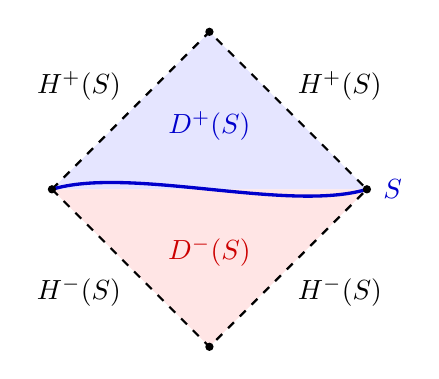
\begin{tikzpicture}[scale=1]
  % D+(S) Region
  \draw[thick, fill=blue!10, dashed] (-2,0) -- (0, 2) -- (2,0);
  % D-(S) Region
  \draw[thick, fill=red!10, dashed] (-2,0) -- (0, -2) -- (2,0);
  
  % Spacelike Surface S
  \draw[very thick, blue!80!black] (-2,0) .. controls (-1, 0.3) and (1, -0.3) .. (2,0) node[right=2pt] {$S$};
  
  % Labels
  \node[blue!80!black, font=\bfseries] at (0, 0.8) {$D^+(S)$};
  \node[red!80!black, font=\bfseries] at (0, -0.8) {$D^-(S)$};
  
  \node[above left] at (-1, 1) {$H^+(S)$};
  \node[above right] at (1, 1) {$H^+(S)$};
  
  \node[below left] at (-1, -1) {$H^-(S)$};
  \node[below right] at (1, -1) {$H^-(S)$};

  \fill (0,2) circle (1.5pt);
  \fill (0,-2) circle (1.5pt);
  \fill (-2,0) circle (1.5pt);
  \fill (2,0) circle (1.5pt);
\end{tikzpicture}
\caption{Domains of dependence and Cauchy horizons for a spacelike surface $S$.}
\label{fig:domain_of_dependence}
\end{figure}

\subsection*{Failures of Causal Structure}
Causal structure can fail dramatically depending on the intrinsic topology and chosen metrics, primarily manifesting in three catastrophic geometrical configurations:

1. \textbf{Poor Choice of Hypersurface:} An otherwise well-behaved spacetime where the specified initial hypersurface is fundamentally incapable of intercepting all causal curves, thus strictly failing to act as a Cauchy surface.
% Drawing 7: Past light cone intersecting an incomplete hypersurface S
\begin{figure}[htbp]
\centering
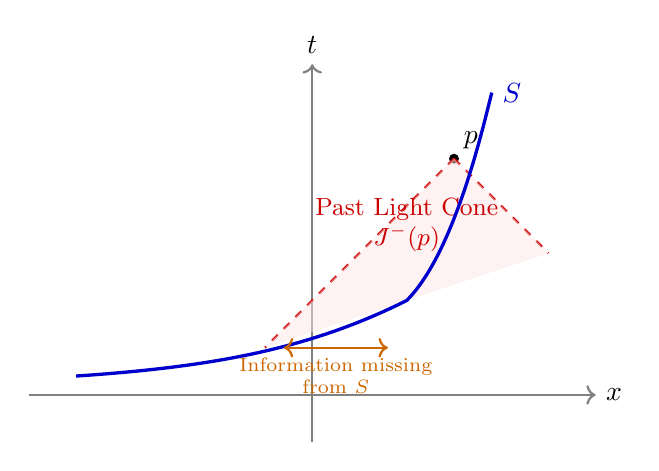
\begin{tikzpicture}[scale=1.2]
  % Axes
  \draw[->, thick, gray] (0,-0.5) -- (0, 3.5) node[above, text=black] {$t$};
  \draw[->, thick, gray] (-3,0) -- (3, 0) node[right, text=black] {$x$};
  
  % Point p
  \coordinate (P) at (1.5, 2.5);
  \fill[black] (P) circle (1.5pt) node[above right] {$p$};
  
  % Past Light Cone of p
  \draw[thick, red!80!black, dashed] (P) -- (-0.5, 0.5);
  \draw[thick, red!80!black, dashed] (P) -- (2.5, 1.5);
  \fill[red!10, opacity=0.5] (P) -- (-0.5, 0.5) -- (2.5, 1.5) -- cycle;
  \node[red!80!black, font=\small, align=center] at (1.0, 1.8) {Past Light Cone\\$J^-(p)$};

  % Hypersurface S (asymptotically approaching a null line, bounded)
  \draw[very thick, blue!80!black] (-2.5, 0.2) .. controls (-1, 0.3) and (0, 0.5) .. (1, 1) .. controls (1.5, 1.5) and (1.8, 2.8) .. (1.9, 3.2) node[right] {$S$};
  
  % Highlight intersection failure
  \draw[<->, thick, orange!80!black] (-0.3, 0.5) -- (0.8, 0.5) node[midway, below, font=\scriptsize, align=center] {Information missing\\from $S$};
\end{tikzpicture}
\caption{An incomplete Cauchy surface $S$ failing to capture the full past of $p$.}
\label{fig:incomplete_cauchy}
\end{figure}

2. \textbf{Closed Timelike Curves (CTCs):} In complex topologies such as $R \times S^1$, the metric signature allows light cones to functionally "tilt," providing geometrically consistent timelike trajectories that loop back to their own past:
\begin{equation} ds^2 = -\cos(\lambda) dt^2 - \sin(\lambda) (dt dx + dx dt) + \cos(\lambda) dx^2 \end{equation}
% Drawing 8: Tipping light cones and Closed Timelike Curve (CTC)
\begin{figure}[H] % <-- Changed [htbp] to [H]
\centering
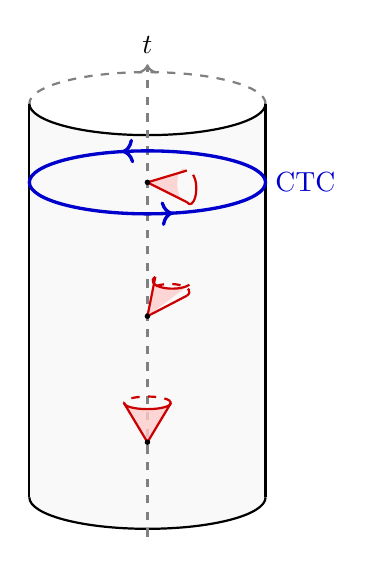
\begin{tikzpicture}[scale=1]
  % Cylinder background (back half)
  \draw[thick, dashed, gray] (1.5, 2.5) arc (0:180:1.5 and 0.4);
  \draw[thick, dashed, gray] (1.5, -2.5) arc (0:180:1.5 and 0.4);
  
  % Cylinder fill
  \path[fill=gray!5] (-1.5,-2.5) -- (-1.5,2.5) arc (180:360:1.5 and 0.4) -- (1.5,-2.5) arc (360:180:1.5 and 0.4) -- cycle;
  
  % Cylinder foreground
  \draw[thick] (-1.5, -2.5) -- (-1.5, 2.5);
  \draw[thick] (1.5, -2.5) -- (1.5, 2.5);
  \draw[thick] (-1.5, 2.5) arc (180:360:1.5 and 0.4);
  \draw[thick] (-1.5, -2.5) arc (180:360:1.5 and 0.4);

  % Axis
  \draw[->, thick, gray, dashed] (0, -3) -- (0, 3) node[above, text=black] {$t$};

  % Upright Light Cone (Bottom)
  \begin{scope}[shift={(0, -1.8)}]
    \fill[red!20, opacity=0.8] (0,0) -- (-0.3, 0.5) arc (180:360:0.3 and 0.08) -- cycle;
    \draw[thick, red!80!black] (0,0) -- (-0.3, 0.5);
    \draw[thick, red!80!black] (0,0) -- (0.3, 0.5);
    \draw[thick, red!80!black] (-0.3, 0.5) arc (180:360:0.3 and 0.08);
    \draw[thick, red!80!black, dashed] (0.3, 0.5) arc (0:180:0.3 and 0.08);
    \fill (0,0) circle (1pt);
  \end{scope}

  % Tilted Light Cone (Middle)
  \begin{scope}[shift={(0, -0.2)}]
    \fill[red!20, opacity=0.8] (0,0) -- (0.1, 0.5) arc (150:330:0.25 and 0.1) -- cycle;
    \draw[thick, red!80!black] (0,0) -- (0.1, 0.5);
    \draw[thick, red!80!black] (0,0) -- (0.5, 0.26);
    \draw[thick, red!80!black] (0.1, 0.5) arc (150:330:0.25 and 0.1);
    \draw[thick, red!80!black, dashed] (0.5, 0.26) arc (-30:150:0.25 and 0.1);
    \fill (0,0) circle (1pt);
  \end{scope}

  % Tipped Light Cone (Top - tangent to CTC)
  \begin{scope}[shift={(0, 1.5)}]
    \fill[red!20, opacity=0.8] (0,0) -- (0.5, 0.15) arc (60:240:0.08 and 0.2) -- cycle;
    \draw[thick, red!80!black] (0,0) -- (0.5, 0.15);
    \draw[thick, red!80!black] (0,0) -- (0.5, -0.25);
    \draw[thick, red!80!black] (0.5, -0.25) arc (240:420:0.08 and 0.2);
    \fill (0,0) circle (1pt);
  \end{scope}

  % Closed Timelike Curve (CTC) at t = 1.5
  \draw[very thick, blue!80!black, decoration={markings, mark=at position 0.3 with {\arrow{>}}, mark=at position 0.8 with {\arrow{>}}}, postaction={decorate}] (0, 1.5) ellipse (1.5 and 0.4);
  \node[blue!80!black, right] at (1.5, 1.5) {CTC};

\end{tikzpicture}
\caption{Tipping of light cones leading to the formation of a Closed Timelike Curve.}
\label{fig:ctc_cylinder}
\end{figure}

3. \textbf{Singularities:} Points where physical models structurally diverge generate distinct mathematical "edges", creating absolute Cauchy horizons that definitively terminate physical predictability.
% Drawing 9: Singularity and Unpredictable Region beyond Cauchy Horizon
\begin{figure}[H] % 
\centering
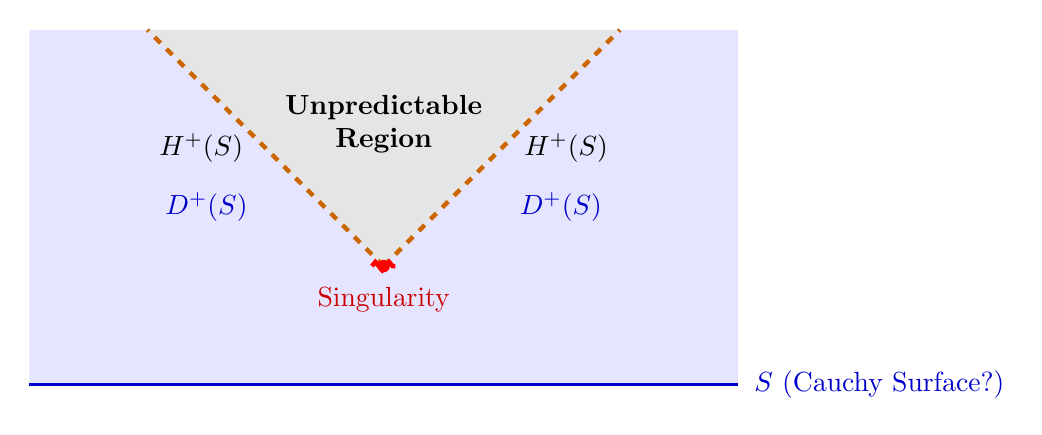
\begin{tikzpicture}[scale=1.5]
  % Future Light Cone of the Singularity (Unpredictable Region)
  \fill[gray!20] (0, 1) -- (-2, 3) -- (2, 3) -- cycle;
  
  % Domain of Dependence D+(S)
  \fill[blue!10] (-3, 0) -- (-3, 3) -- (-2, 3) -- (0, 1) -- (2, 3) -- (3, 3) -- (3, 0) -- cycle;

  % Cauchy Horizon H+(S)
  \draw[ultra thick, dashed, orange!80!black] (0, 1) -- (-2, 3) node[midway, left=4pt, text=black] {$H^+(S)$};
  \draw[ultra thick, dashed, orange!80!black] (0, 1) -- (2, 3) node[midway, right=4pt, text=black] {$H^+(S)$};

  % Singularity
  \draw[ultra thick, decorate, decoration={zigzag, segment length=5pt, amplitude=1.5pt}, red] (-0.1, 1) -- (0.1, 1);
  \fill[red] (0,1) circle (1.5pt);
  \node[red!80!black, below] at (0, 0.9) {Singularity};

  % Spacelike Surface S
  \draw[very thick, blue!80!black] (-3, 0) -- (3, 0) node[right=2pt] {$S$ (Cauchy Surface?)};

  % Labels
  \node[blue!80!black, font=\bfseries] at (-1.5, 1.5) {$D^+(S)$};
  \node[blue!80!black, font=\bfseries] at (1.5, 1.5) {$D^+(S)$};
  
  \node[font=\bfseries, align=center] at (0, 2.2) {Unpredictable\\Region};
  
\end{tikzpicture}
\caption{Breakdown of predictability beyond the Cauchy horizon due to a singularity.}
\label{fig:cauchy_horizon_singularity}
\end{figure}

\section{Tensor Densities}
While true tensors scale cleanly via localized coordinate matrices, density objects scale additionally relative to the full manifold volume transformation, absorbing the Jacobian determinant $|J|^W$. 

\subsection*{The Levi-Civita Symbol and Metric Determinant}
The Levi-Civita permutation symbol analytically absorbs exactly one factor of the Jacobian determinant, effectively acquiring a weight of $W=+1$:
\begin{equation} \tilde{\epsilon}_{\mu'_1 \dots \mu'_n} = |J| \left( \tilde{\epsilon}_{\mu_1 \dots \mu_n} \frac{\partial x^{\mu_1}}{\partial x^{\mu'_1}} \dots \frac{\partial x^{\mu_n}}{\partial x^{\mu'_n}} \right) \end{equation}
Concurrently, calculating the transformation determinant of the full metric tensor mathematically yields a strict density of weight $W=-2$:
\begin{equation} g' = (|J|^{-1})^2 g \implies g' = |J|^{-2} g \end{equation}

\subsection*{The Levi-Civita Tensor}
By mathematically combining these disparate densities, we synthesize a mathematically true tensorial object. Factoring in $\sqrt{|g|}$ ($W=-1$) perfectly cancels the permutation weight, manifesting the invariant Levi-Civita Tensor:
\begin{equation} \epsilon_{\mu_1\mu_2\dots\mu_n} = \sqrt{|g|} \tilde{\epsilon}_{\mu_1\mu_2\dots\mu_n} \end{equation}
The contravariant execution involves standard index raising via the metric inverse:
\begin{equation} \epsilon^{\mu_1\mu_2\dots\mu_n} = \frac{1}{\sqrt{|g|}} \tilde{\epsilon}^{\mu_1\mu_2\dots\mu_n} \end{equation}

\subsection*{Contraction Identity}
Contracting corresponding tensor indices significantly reduces computational complexity, analytically generating arrays of scaled Kronecker deltas proportional to the contraction depth:
\begin{equation} \epsilon^{\mu_1\dots\mu_n} \epsilon_{\nu_1\dots\nu_n} = (-1)^s \tilde{\epsilon}^{\mu_1\dots\mu_n} \tilde{\epsilon}_{\nu_1\dots\nu_n} \end{equation}
\begin{equation} \tilde{\epsilon}^{\mu_1\dots\mu_n} \tilde{\epsilon}_{\nu_1\dots\nu_n} = \delta^{\mu_1\dots\mu_n}_{\nu_1\dots\nu_n} = n! \delta^{[\mu_1}_{\nu_1} \dots \delta^{\mu_n]}_{\nu_n} \end{equation}
For a generalized $p$-index contraction:
\begin{equation} \epsilon^{\mu_1\dots\mu_p\alpha_1\dots} \epsilon_{\mu_1\dots\mu_p\beta_1\dots} = (-1)^s p!(n-p)! \delta^{[\alpha_1}_{\beta_1} \dots \delta^{\alpha_{n-p}]}_{\beta_{n-p}} \end{equation}
The highest utility physical application ($p=n-1$) produces a direct algebraic trace:
\begin{equation} \epsilon^{\mu_1\dots\mu_{n-1}\alpha} \epsilon_{\mu_1\dots\mu_{n-1}\beta} = (-1)^s (n-1)! \delta^\alpha_\beta \end{equation}

\section{Differential Forms}
The rigorous foundation of volume integration relies upon $p$-forms, which natively manifest as totally antisymmetric covariant $(0,p)$ tensors.

\subsection*{The Wedge Product and Exterior Derivative}
The mathematical fusion of independent forms is administered by the wedge product, ensuring total internal antisymmetry:
\begin{equation} (A \wedge B)_{\mu_1 \dots \mu_{p+q}} = \frac{(p+q)!}{p!q!} A_{[\mu_1 \dots \mu_p} B_{\mu_{p+1} \dots \mu_{p+q}]} \end{equation}
\begin{equation} A \wedge B = (-1)^{pq} B \wedge A \end{equation}
The application of the exterior derivative geometrically extends a $p$-form directly into a structurally complex $(p+1)$-form:
\begin{equation} (dA)_{\mu_1 \dots \mu_{p+1}} = (p+1) \partial_{[\mu_1} A_{\mu_2 \dots \mu_{p+1}]} \end{equation}
\begin{equation} d(A \wedge B) = (dA) \wedge B + (-1)^p A \wedge (dB) \end{equation}
Crucially, the exterior derivative $dA$ transforms analytically as an exact true tensor because the problematic non-tensorial second derivatives within the partial expansion are identically symmetric, strictly forcing cancellation under the wedge product's internal antisymmetrization. This inherent symmetry guarantees that all exact physical forms are strictly closed mathematically:
\begin{equation} d(dA) = 0 \end{equation}

\subsection*{The Double Dual Identity}
Applying the Hodge Star twice over recovers the original tensor up to a predictable structural sign factor corresponding to index signatures and dimensionality:
\begin{equation} \star\star A = (-1)^{s + p(n-p)} A \end{equation}

\subsection*{Maxwell's Equations}
The profound structural advantages of differential forms are beautifully evidenced by the condensation of classical electromagnetism into pure geometry. Using the Faraday 2-form $F = dA$, the entirety of Maxwell's field logic becomes exact, completely coordinate-free exterior geometry:
\begin{equation} dF = d(dA) = 0 \end{equation}
\begin{equation} d(\star F) = \star J \end{equation}
Translating directly via the Hodge dual recovers the familiar covariant classical formulation identically:
\begin{equation} \nabla_\mu F^{\mu\nu} = J^\nu \end{equation}

\section{Integration}
Generalizing formal integration to curved space necessitates a localized volume element that successfully bypasses the distorting impacts of coordinate variance. The standard numerical integration measure behaves identically to a pure density weighting ($W=+1$):
\begin{equation} d^n x' = \left| \frac{\partial x^{\mu'}}{\partial x^\mu} \right| d^n x = |J| d^n x \end{equation}
Subsequently, the true integration operation serves exclusively as a functional mapping scaling an exact $n$-form cleanly into a real-valued scalar output:
\begin{equation} \int_\Sigma : \omega \to \mathbb{R} \end{equation}

% Drawing 1: 3D Volume Element / Basis Vectors
\begin{figure}[htbp]
\centering
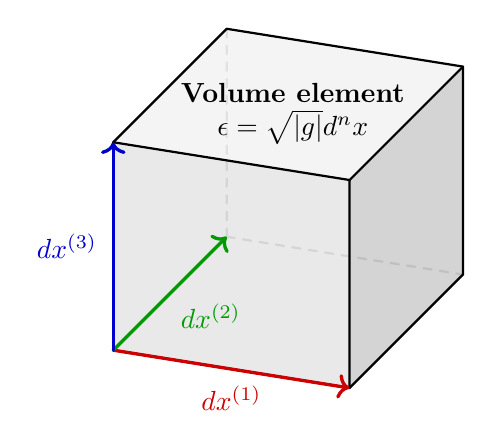
\begin{tikzpicture}[scale=1.2, line join=round, line cap=round]
  % Define origin and basis vectors
  \coordinate (O) at (0,0);
  \coordinate (V1) at (2.5, -0.4);
  \coordinate (V2) at (1.2, 1.2);
  \coordinate (V3) at (0, 2.2);

  % Calculate vertices
  \coordinate (V12) at ($(V1)+(V2)$);
  \coordinate (V13) at ($(V1)+(V3)$);
  \coordinate (V23) at ($(V2)+(V3)$);
  \coordinate (V123) at ($(V1)+(V2)+(V3)$);

  % Draw hidden (back) edges
  \draw[thick, dashed, gray] (O) -- (V2);
  \draw[thick, dashed, gray] (V2) -- (V12);
  \draw[thick, dashed, gray] (V2) -- (V23);

  % Fill visible faces with varying opacity for 3D effect
  \fill[gray!20, opacity=0.85] (O) -- (V1) -- (V13) -- (V3) -- cycle; % Front
  \fill[gray!40, opacity=0.85] (V1) -- (V12) -- (V123) -- (V13) -- cycle; % Right
  \fill[gray!10, opacity=0.85] (V3) -- (V13) -- (V123) -- (V23) -- cycle; % Top

  % Draw visible edges
  \draw[thick] (O) -- (V1) -- (V12) -- (V123) -- (V23) -- (V3) -- cycle;
  \draw[thick] (V1) -- (V13) -- (V3);
  \draw[thick] (V13) -- (V123);

  % Draw the three primary vectors
  \draw[->, very thick, red!80!black] (O) -- (V1) node[midway, below=2pt] {$dx^{(1)}$};
  \draw[->, very thick, green!60!black] (O) -- (V2) node[midway, below right] {$dx^{(2)}$};
  \draw[->, very thick, blue!80!black] (O) -- (V3) node[midway, left=2pt] {$dx^{(3)}$};

  % Label the volume
\node[font=\bfseries, align=center] at (1.9, 2.5) {Volume element \\ $\epsilon = \sqrt{|g|} d^n x$};
\end{tikzpicture}
\caption{The invariant volume element in a curved space.}
\label{fig:volume_element}
\end{figure}

\subsection*{The Invariant Volume Element}
By algebraically combining the metric determinant scaling ($\sqrt{|g|}$ with weight $W=-1$) alongside the raw numerical expansion element ($d^n x$ with weight $W=+1$), a fundamentally invariant physical $n$-form is achieved:
\begin{equation} \epsilon = \sqrt{|g|} d^n x \end{equation}
This rigorous construction ensures that global volumetric action scalar integrals behave physically and identically invariant across all topological mappings and independent frames:
\begin{equation} S = \int \phi(x) \sqrt{|g|} d^n x = \int \phi(x) \epsilon \end{equation}

\chapter{Curvature}

\section{Overview}
The transition from a flat Minkowski spacetime to a dynamic, curved manifold necessitates a rigorous mathematical framework to quantify deviations from flat-space geometry. The intrinsic curvature of spacetime is definitively measured by the Riemann tensor, which is constructed systematically through a hierarchy of geometric structures:

\textbf{1. The Connection (Christoffel Symbols):} A mathematical object that bridges disjoint tangent spaces, enabling the comparison of vectors at infinitesimally separated points.
\begin{equation}\label{eq:christoffel_preview}
\Gamma_{\mu\nu}^{\lambda} = \frac{1}{2}g^{\lambda\sigma} (\partial_{\mu}g_{\nu\sigma} + \partial_{\nu}g_{\sigma\mu} - \partial_{\sigma}g_{\mu\nu})
\end{equation}

\textbf{2. The Covariant Derivative:} An extension of the standard partial derivative that guarantees tensorial transformation properties across curved coordinate grids.
\begin{equation}\label{eq:cov_deriv_preview}
\nabla_{\mu}V^{\nu} = \partial_{\mu}V^{\nu} + \Gamma_{\mu\sigma}^{\nu}V^{\sigma}
\end{equation}

\textbf{3. Geodesics:} The geometric generalization of straight lines, representing the unaccelerated, freely-falling trajectories of particles in a gravitational field.
\begin{equation}\label{eq:geodesic_preview}
\frac{d^{2}x^{\mu}}{d\lambda^{2}} + \Gamma_{\rho\sigma}^{\mu} \frac{dx^{\rho}}{d\lambda} \frac{dx^{\sigma}}{d\lambda} = 0
\end{equation}

\textbf{4. The Riemann Curvature Tensor:} A rank-4 tensor that encapsulates the non-commutativity of covariant derivatives, providing the definitive, coordinate-independent measure of true curvature.
\begin{equation}\label{eq:riemann_preview}
{R^{\rho}}_{\sigma\mu\nu} = \partial_{\mu}\Gamma_{\nu\sigma}^{\rho} - \partial_{\nu}\Gamma_{\mu\sigma}^{\rho} + \Gamma_{\mu\lambda}^{\rho}\Gamma_{\nu\sigma}^{\lambda} - \Gamma_{\nu\lambda}^{\rho}\Gamma_{\mu\sigma}^{\lambda}
\end{equation}

\section{Covariant Derivatives}
In a curved manifold, the basis vectors characterizing the coordinate grid vary from point to point. Consequently, the standard partial derivative of a tensor component fails to transform as a true tensor, as the transformation law produces an anomalous second-derivative term dependent on the coordinate choice.

\subsection*{Defining the Covariant Derivative}
To rectify this, the covariant derivative $\nabla_\mu$ is introduced. By incorporating the connection coefficients $\Gamma$, the covariant derivative functionally absorbs the variation of the basis vectors, ensuring the resultant object remains strictly tensorial:
\begin{equation}\label{eq:cov_deriv_vector}
\nabla_\mu V^\nu = \partial_\mu V^\nu + \Gamma^\nu_{\mu\lambda} V^\lambda
\end{equation}
Enforcing the strict tensorial transformation law on $\nabla_\mu V^\nu$ dictates the specific, non-tensorial transformation rule that the connection coefficients must obey:
\begin{equation}\label{eq:gamma_transformation}
\Gamma^{\nu'}_{\mu'\lambda'} = \frac{\partial x^\mu}{\partial x^{\mu'}} \frac{\partial x^\lambda}{\partial x^{\lambda'}} \frac{\partial x^{\nu'}}{\partial x^\nu} \Gamma^\nu_{\mu\lambda} - \frac{\partial x^\mu}{\partial x^{\mu'}} \frac{\partial x^{\lambda}}{\partial x^{\lambda'}} \frac{\partial^2 x^{\nu'}}{\partial x^\mu \partial x^\lambda}
\end{equation}

To preserve the fundamental Leibniz (product) rule for tensor contraction, the covariant derivative of a dual vector (one-form) $\omega_\lambda$ naturally requires a corresponding negative connection term:
\begin{equation}
\nabla_\mu \omega_\lambda = \partial_\mu \omega_\lambda - \Gamma^\sigma_{\mu\lambda} \omega_\sigma
\end{equation}

\subsection*{The Christoffel Connection}
While any manifold admits an infinite number of possible connections, general relativity uniquely selects the Levi-Civita connection. This specific connection is defined by two physical requirements: it is torsion-free ($\Gamma^\lambda_{\mu\nu} = \Gamma^\lambda_{\nu\mu}$), and it is metric-compatible, meaning the covariant derivative of the metric tensor identically vanishes ($\nabla_\rho g_{\mu\nu} = 0$). 

Metric compatibility ensures that the inner product of two vectors remains invariant under parallel transport. By cyclically permuting the indices of the metric compatibility condition and utilizing the torsion-free symmetry, one derives the Christoffel symbols directly from the metric derivatives:
\begin{equation}\label{eq:christoffel_formula}
\Gamma^\sigma_{\mu\nu} = \frac{1}{2} g^{\sigma\rho} ( \partial_\mu g_{\nu\rho} + \partial_\nu g_{\rho\mu} - \partial_\rho g_{\mu\nu} )
\end{equation}

\subsection*{Divergence Formula}
Evaluating the trace of the Christoffel symbol yields a fundamental identity linking the connection to the determinant of the metric $g$. This identity is crucial for formulating conservation laws in curved spacetime:
\begin{equation}\label{eq:gamma_contracted}
\Gamma^\mu_{\mu\lambda} = \frac{1}{\sqrt{|g|}} \partial_\lambda \sqrt{|g|}
\end{equation}
Applying this identity allows the covariant divergence of a vector field to be expressed purely in terms of partial derivatives and the metric determinant, thereby generalizing Stokes' theorem to curved manifolds:
\begin{equation}
\nabla_\mu V^\mu = \frac{1}{\sqrt{|g|}} \partial_\mu (\sqrt{|g|} V^\mu)
\end{equation}
\begin{equation}
\int_{\mathcal{V}} d^n x \sqrt{|g|} \nabla_\mu V^\mu = \int_{\partial \mathcal{V}} d^{n-1} x \sqrt{|\gamma|} n_\mu V^\mu
\end{equation}

\section{Parallel Transport and Geodesics}

% Drawing 2: Parallel Transport on a Sphere
\begin{figure}[htbp]
\centering
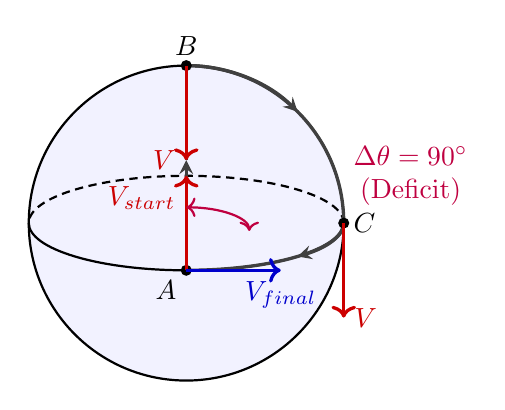
\begin{tikzpicture}[scale=2]
  % Sphere Base
  \draw[thick, fill=blue!5] (0,0) circle (1);
  
  % Equator
  \draw[thick, densely dashed] (1,0) arc (0:180:1 and 0.3);
  \draw[thick] (-1,0) arc (180:360:1 and 0.3);

  % Geodesic Paths
  % Path A -> B (Central Meridian)
  \draw[very thick, darkgray, -stealth] (0,-0.3) -- (0, 0.4);
  \draw[very thick, darkgray] (0,0.4) -- (0,1);
  
  % Path B -> C (Right Meridian)
  \draw[very thick, darkgray, -stealth] (0,1) arc (90:45:1 and 1);
  \draw[very thick, darkgray] (0,1) arc (90:0:1 and 1);
  
  % Path C -> A (Equator segment)
  \draw[very thick, darkgray, -stealth] (1,0) arc (360:315:1 and 0.3);
  \draw[very thick, darkgray] (1,0) arc (360:270:1 and 0.3);

  % Key Points
  \fill (0,-0.3) circle (1pt) node[below left] {$A$};
  \fill (0,1) circle (1pt) node[above] {$B$};
  \fill (1,0) circle (1pt) node[right] {$C$};

  % Transported Vectors
  % Initial Vector at A (Pointing North)
  \draw[->, very thick, red!80!black] (0,-0.3) -- (0, 0.3) node[below left] {$V_{start}$};
  
  % Vector transported to B (Points South along central meridian)
  \draw[->, very thick, red!80!black] (0,1) -- (0, 0.4) node[left] {$V$};
  
  % Vector transported to C (Maintains angle with meridian, points South)
  \draw[->, very thick, red!80!black] (1,0) -- (1, -0.6) node[right] {$V$};
  
  % Vector returned to A (Parallel to equator, points East)
  \draw[->, very thick, blue!80!black] (0,-0.3) -- (0.6, -0.3) node[below] {$V_{final}$};

  % Highlight Deficit Angle at A
  \draw[<->, thick, purple] (0, 0.1) arc (90:0:0.4 and 0.15);
  \node[purple, right, align=center] at (1, 0.3) {$\Delta\theta = 90^\circ$ \\ (Deficit)};
\end{tikzpicture}
\caption{Parallel transport on a sphere resulting in a deficit angle.}
\label{fig:parallel_transport_sphere}
\end{figure}

Because tangent spaces at distinct points are disjoint, moving a vector continuously along a curve without intrinsically altering its orientation requires a formal geometric procedure known as parallel transport. A vector $V^\mu$ is parallel transported along a curve parameterized by $\lambda$ if its directional covariant derivative along the curve vanishes:
\begin{equation}\label{eq:parallel_transport}
\frac{D V^\mu}{d\lambda} \equiv \frac{dx^\nu}{d\lambda} \nabla_\nu V^\mu = 0 \implies \frac{d V^\mu}{d\lambda} + \Gamma^\mu_{\sigma\rho} \frac{dx^\sigma}{d\lambda} V^\rho = 0
\end{equation}

\subsection*{Geodesic Equation}
A geodesic is defined geometrically as an auto-parallel curve; it is a path that parallel transports its own tangent vector $U^\mu = dx^\mu/d\lambda$. Setting $V^\mu = U^\mu$ in the parallel transport equation yields the fundamental geodesic equation, governing the motion of free-falling particles:
\begin{equation}\label{eq:geodesic_eq}
\frac{d^2 x^\mu}{d\lambda^2} + \Gamma^\mu_{\rho\sigma} \frac{dx^\rho}{d\lambda} \frac{dx^\sigma}{d\lambda} = 0
\end{equation}

\subsection*{Variational Principle}
Alternatively, timelike geodesics can be derived physically by extremizing the proper time (or energy integral) between two events. By defining the action $I = \frac{1}{2} \int g_{\mu\nu} \dot{x}^\mu \dot{x}^\nu d\tau$ and applying the Euler-Lagrange equations, the equations of motion natively recover the Christoffel symbols and the exact geodesic formulation:
\begin{equation}
g_{\sigma\nu} \ddot{x}^\nu + \frac{1}{2} \left( \partial_\mu g_{\sigma\nu} + \partial_\nu g_{\sigma\mu} - \partial_\sigma g_{\mu\nu} \right) \dot{x}^\mu \dot{x}^\nu = 0
\end{equation}

\subsection*{Null Geodesics}
Massless particles, such as photons, follow null geodesics where the spacetime interval vanishes ($ds^2 = 0$). Since proper time cannot parameterize a null path, an affine parameter $\lambda$ is utilized such that the four-momentum is $p^\mu = dx^\mu/d\lambda$. The geodesic equation remains structurally identical:
\begin{equation}
p^\nu \nabla_\nu p^\mu = 0
\end{equation}

\section{Properties of Geodesics}

\subsection*{Affine Parameters}
The parameterization of a geodesic is strictly constrained. An affine parameter $\lambda$ ensures that the right-hand side of the geodesic equation remains exactly zero. Under an arbitrary reparameterization $\alpha(\lambda)$, the auto-parallel condition is only maintained if the transformation is strictly linear ($\alpha = a\lambda + b$), enforcing $d^2\alpha/d\lambda^2 = 0$:
\begin{equation}
\left( \frac{d\alpha}{d\lambda} \right)^2 \left[ \frac{d^2 x^\mu}{d\alpha^2} + \Gamma^\mu_{\rho\sigma} \frac{dx^\rho}{d\alpha} \frac{dx^\sigma}{d\alpha} \right] + \frac{dx^\mu}{d\alpha} \frac{d^2\alpha}{d\lambda^2} = 0
\end{equation}

\subsection*{Riemann Normal Coordinates (RNC)}
Around any non-singular point $p$, the exponential map facilitates the construction of Riemann Normal Coordinates (RNC). In this locally inertial frame, all geodesics passing through $p$ appear as Euclidean straight lines. Consequently, the first derivatives of the metric vanish, forcing the connection coefficients to equal zero exactly at $p$:
\begin{equation}
\Gamma^{\hat{\mu}}_{\hat{\rho}\hat{\sigma}}(p) = 0 \implies \partial_{\hat{\rho}} g_{\hat{\mu}\hat{\nu}}(p) = 0
\end{equation}

\section{The Expanding Universe Revisited}
To demonstrate the utility of the connection framework, consider the spatially flat Robertson-Walker (RW) cosmological metric, which models a homogeneous and isotropic expanding universe parameterized by the scale factor $a(t)$:
\begin{equation}
ds^2 = -dt^2 + a^2(t) \delta_{ij} dx^i dx^j
\end{equation}
Applying the variational principle to the metric Lagrangian directly extracts the non-vanishing connection coefficients without computing individual metric derivatives:
\begin{align}
\Gamma^0_{00} &= 0, \quad \Gamma^0_{0i} = 0, \quad \Gamma^0_{ij} = a\dot{a} \delta_{ij}, \\
\Gamma^k_{0j} &= \frac{\dot{a}}{a} \delta^k_j, \quad \Gamma^k_{ij} = 0, \quad \Gamma^k_{00} = 0
\end{align}

\subsection*{Cosmological Redshift}
The expansion of the universe physically stretches the wavelength of propagating light. By evaluating the $t$-component of the geodesic equation for a null trajectory, the differential equation dictates that the observed frequency (and corresponding energy) is inversely proportional to the scale factor:
\begin{equation}
\frac{d}{d\lambda} \ln \left( \frac{dt}{d\lambda} \right) = - \frac{d}{d\lambda} \ln a \implies \frac{dt}{d\lambda} = \frac{\omega_0}{a(t)}
\end{equation}

\subsection*{Conservation of Energy-Momentum}
Imposing the covariant conservation law ($\nabla_\mu T^{\mu\nu} = 0$) upon a perfect fluid in the RW background yields the cosmological continuity equation, precisely defining how the energy density $\rho$ dilutes as the manifold expands:
\begin{equation}
\dot{\rho} + 3\frac{\dot{a}}{a} (\rho + p) = 0
\end{equation}

\section{The Riemann Curvature Tensor}


% Drawing 3: Riemann Curvature Deficit Vector Loop
\begin{figure}[htbp]
\centering
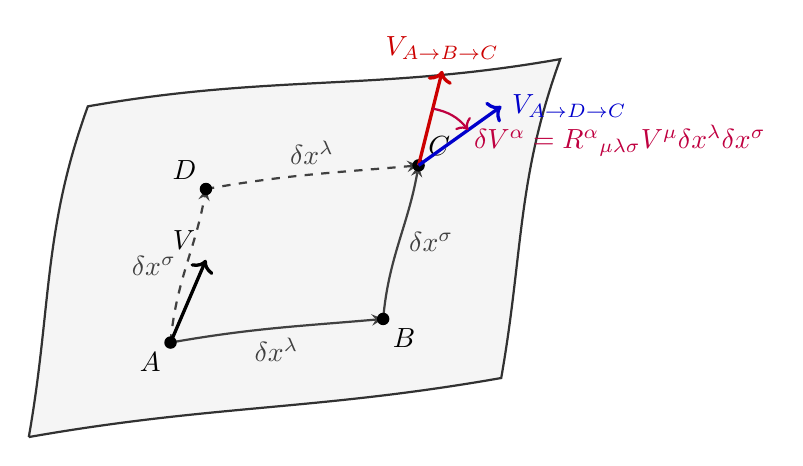
\begin{tikzpicture}[scale=1.5]
  % Curved surface patch
  \draw[thick, fill=gray!10, opacity=0.8] (0,0) to[out=10, in=190] (4,0.5) 
        to[out=80, in=250] (4.5,3.2) 
        to[out=190, in=10] (0.5,2.8) 
        to[out=250, in=80] (0,0);

  % Loop Coordinates
  \coordinate (A) at (1.2, 0.8);
  \coordinate (B) at (3.0, 1.0);
  \coordinate (C) at (3.3, 2.3);
  \coordinate (D) at (1.5, 2.1);

  % Loop Paths (A->B->C and A->D->C)
  \draw[thick, darkgray, -stealth] (A) to[out=10, in=185] node[midway, below] {$\delta x^\lambda$} (B);
  \draw[thick, darkgray, -stealth] (B) to[out=85, in=260] node[midway, right] {$\delta x^\sigma$} (C);
  \draw[thick, darkgray, dashed, -stealth] (A) to[out=85, in=260] node[midway, left] {$\delta x^\sigma$} (D);
  \draw[thick, darkgray, dashed, -stealth] (D) to[out=10, in=185] node[midway, above] {$\delta x^\lambda$} (C);

  % Vertices
  \fill (A) circle (1.5pt) node[below left] {$A$};
  \fill (B) circle (1.5pt) node[below right] {$B$};
  \fill (C) circle (1.5pt) node[above right] {$C$};
  \fill (D) circle (1.5pt) node[above left] {$D$};

  % Initial Vector at A
  \draw[->, very thick, black] (A) -- ++(0.3, 0.7) node[above left] {$V$};

  % Transported Vectors at C
  \coordinate (V1) at ($(C) + (0.2, 0.8)$); % Transported via B
  \coordinate (V2) at ($(C) + (0.7, 0.5)$); % Transported via D

  \draw[->, very thick, red!80!black] (C) -- (V1) node[above] {$V_{A \to B \to C}$};
  \draw[->, very thick, blue!80!black] (C) -- (V2) node[right] {$V_{A \to D \to C}$};

  % Riemann Curvature Deficit Vector
  \draw[->, thick, purple] ($(C)!0.6!(V1)$) to[bend left=20] node[below=9pt, right=4pt] {$\delta V^\alpha = R^\alpha{}_{\mu\lambda\sigma} V^\mu \delta x^\lambda \delta x^\sigma$} ($(C)!0.6!(V2)$);
\end{tikzpicture}
\caption{Riemann curvature defined by parallel transport around a closed loop.}
\label{fig:riemann_curvature}
\end{figure}


Intrinsic curvature manifests mathematically as the non-commutativity of the covariant derivative. Evaluating the commutator of second covariant derivatives on an arbitrary vector field generates a linear transformation proportional to the vector itself. For a torsion-free connection, the coefficient of this transformation strictly defines the Riemann curvature tensor ${R^\rho}_{\sigma\mu\nu}$:
\begin{equation}\label{eq:riemann_def}
[\nabla_\mu, \nabla_\nu] V^\rho = {R^\rho}_{\sigma\mu\nu} V^\sigma
\end{equation}
Physically, the Riemann tensor quantifies the exact deficit vector $\delta V^{\alpha}$ produced when a vector is parallel transported around an infinitesimal closed loop spanned by variations $\delta x^\lambda$ and $\delta x^\sigma$:
\begin{equation}
\delta V^{\alpha} = {R^{\alpha}}_{\mu\lambda\sigma} V^{\mu} \delta x^{\lambda} \delta x^{\sigma}
\end{equation}

\subsection*{Theorem: Flatness}
A manifold is defined as globally flat if and only if the Riemann tensor vanishes identically everywhere ($R^\rho{}_{\sigma\mu\nu} = 0$). This condition mathematically guarantees the existence of a global coordinate system where the metric components are constant ($\partial_\sigma g_{\mu\nu} = 0$), recovering the flat spacetime geometry of special relativity.

\section{Properties of the Riemann Tensor}
\subsection*{Symmetries}
The geometric structure of the manifold heavily restricts the independent degrees of freedom within the Riemann tensor. By evaluating the tensor in Riemann Normal Coordinates, where the connection vanishes and partial derivatives act purely on the metric, the following algebraic symmetries are rigorously established:
\begin{align}
R_{\rho\sigma\mu\nu} &= -R_{\sigma\rho\mu\nu} \quad (\text{Antisymmetry on the first pair}) \\
R_{\rho\sigma\mu\nu} &= -R_{\rho\sigma\nu\mu} \quad (\text{Antisymmetry on the last pair}) \\
R_{\rho\sigma\mu\nu} &= R_{\mu\nu\rho\sigma} \quad (\text{Symmetry under pair exchange}) \\
R_{\rho[\sigma\mu\nu]} &= 0 \quad (\text{First Bianchi Identity})
\end{align}
In a four-dimensional spacetime, these rigid algebraic constraints reduce the initially $256$ independent tensor components to exactly $20$.

\subsection*{Second Bianchi Identity}
Differentiating the Riemann tensor and exploiting the cyclic symmetry of the indices yields the Second Bianchi Identity, a profound differential constraint that fundamentally governs the conservation of energy and momentum in general relativity:
\begin{equation}
\nabla_{[\lambda} R_{\rho\sigma]\mu\nu} = 0
\end{equation}

\subsection*{Ricci, Einstein, and Weyl Tensors}
The exhaustive description of curvature provided by the Riemann tensor is often decomposed into specific scalar and tensorial contractions to isolate physically relevant phenomena.

\textbf{Ricci Tensor and Scalar:} Represents the volume-changing aspect of curvature, derived by tracing the Riemann tensor:
\begin{equation}
R_{\mu\nu} = {R^\lambda}_{\mu\lambda\nu}, \quad R = g^{\mu\nu} R_{\mu\nu}
\end{equation}

\textbf{Einstein Tensor:} By contracting the Second Bianchi Identity twice, one constructs the divergence-free Einstein tensor, which serves as the precise geometric counterpart to the conserved energy-momentum tensor in the field equations:
\begin{equation}
G_{\mu\nu} = R_{\mu\nu} - \frac{1}{2} R g_{\mu\nu}, \quad \nabla^\mu G_{\mu\nu} = 0
\end{equation}

\textbf{Weyl Tensor:} The totally trace-free component of the Riemann tensor, which purely isolates the shape-distorting (tidal) aspects of gravity, describing curvature that propagates through vacuums (such as gravitational waves):
\begin{equation}
C_{\rho\sigma\mu\nu} = R_{\rho\sigma\mu\nu} - \frac{2}{n-2} (g_{\rho[\mu} R_{\nu]\sigma} - g_{\sigma[\mu} R_{\nu]\rho}) + \frac{2}{(n-1)(n-2)} g_{\rho[\mu} g_{\nu]\sigma} R
\end{equation}

\section{Mathematical Interlude: Diffeomorphisms and Lie Derivatives}
While the covariant derivative requires a formally defined metric or connection, the Lie Derivative $\mathcal{L}_V$ provides a manifold-native technique to evaluate the rate of change of a tensor field purely along the flow lines of a vector field $V^\mu$. The operations naturally incorporate the metric-independent commutator:
\begin{align}
\mathcal{L}_V U^\mu &= [V, U]^\mu = V^\nu \partial_\nu U^\mu - U^\nu \partial_\nu V^\mu \\
\mathcal{L}_V \omega_\mu &= V^\nu \partial_\nu \omega_\mu + \omega_\nu \partial_\mu V^\nu \\
\mathcal{L}_V {T^\mu}_\nu &= V^\lambda \nabla_\lambda {T^\mu}_\nu - (\nabla_\lambda V^\mu) {T^\lambda}_\nu + (\nabla_\nu V^\lambda) {T^\mu}_\lambda
\end{align}

\section{Symmetries and Killing Vectors}
Continuous geometric symmetries within a spacetime manifold manifest mathematically when the metric tensor remains invariant along a specific directional flow ($\partial_{\sigma_*} g_{\mu\nu} = 0$). According to Noether's theorem, this geometric invariance guarantees a conserved dynamical quantity for a particle traveling along a geodesic.

If a vector field $K^\mu$ strictly generates such a symmetry flow, the projection of a particle's momentum along this field ($K^\nu p_\nu$) is an absolute constant of motion:
\begin{equation}
\frac{d}{d\tau} (K_\nu p^\nu) = p^\mu p^\nu \nabla_{(\mu} K_{\nu)} = 0
\end{equation}
Because this conservation must hold universally for all possible geodesic trajectories (arbitrary $p^\mu$), the symmetric part of the covariant derivative of the generator must identically vanish. This establishes \textbf{Killing's Equation}, the definitive criteria for a Killing vector field:
\begin{equation}\label{eq:killing_eq}
\nabla_{(\mu} K_{\nu)} = \frac{1}{2} (\nabla_\mu K_\nu + \nabla_\nu K_\mu) = 0
\end{equation}


\chapter{Gravitation}

\section{Physics in Curved Spacetime}

In the Newtonian framework, gravitation is conceptualized as an instantaneous scalar potential field $\Phi$. The dynamical response of a massive body and the generation of the potential by a mass density $\rho$ are governed, respectively, by the local acceleration and Poisson's equation:
\begin{equation}
\label{eq:newton_accel}
\mathbf{a} = -\nabla\Phi \quad \implies \quad \frac{d^{2}x^{i}}{dt^{2}} = -\partial_{i}\Phi
\end{equation}
\begin{equation}
\label{eq:poisson}
\nabla^{2}\Phi = 4\pi G\rho
\end{equation}

\subsection*{The Minimal-Coupling Principle}
To transition these classical concepts into the relativistic domain, we rely on the Einstein Equivalence Principle (EEP). Geometrically, the EEP asserts that spacetime is locally flat. Mathematically, this motivates the minimal-coupling principle (often colloquially termed the "comma-goes-to-semicolon rule"): physical laws valid in special relativity are generalized to curved spacetime by replacing the flat Minkowski metric $\eta_{\mu\nu}$ with the dynamic metric $g_{\mu\nu}$, and partial derivatives $\partial_{\mu}$ with covariant derivatives $\nabla_{\mu}$.

\subsection*{Derivation of the Geodesic Equation}
In the absence of external forces, a free particle in flat spacetime travels along a straight Euclidean line, characterized by zero acceleration with respect to an affine parameter $\lambda$:
\begin{equation}
\label{eq:flat_motion}
\frac{d^{2}x^{\mu}}{d\lambda^{2}} = 0
\end{equation}
By expressing this flat-space trajectory in terms of a directional derivative along the tangent vector $dx^\mu/d\lambda$, and subsequently promoting the partial derivative to its covariant counterpart via the minimal-coupling principle ($\partial_{\nu} \rightarrow \nabla_{\nu}$), we inherently account for the curvature of the coordinate grid. Expanding the covariant derivative introduces the Christoffel connection, yielding the rigorous \textbf{geodesic equation}:
\begin{equation}
\label{eq:geodesic_derivation}
\frac{d^{2}x^{\mu}}{d\lambda^{2}} + \Gamma^{\mu}_{\rho\sigma}\frac{dx^{\rho}}{d\lambda}\frac{dx^{\sigma}}{d\lambda} = 0
\end{equation}
Physically, this equation dictates that a particle in free fall experiences no proper acceleration, tracing out the straightest possible path (an auto-parallel curve) through a curved spacetime geometry.

\subsection*{Energy-Momentum Conservation}
Applying minimal coupling to the local conservation of energy and momentum in special relativity ($\partial_{\mu}T^{\mu\nu} = 0$) elegantly produces the curved-spacetime conservation law:
\begin{equation}
\nabla_{\mu}T^{\mu\nu} = 0
\end{equation}

\subsection*{The Newtonian Limit}
General relativity must reduce to Newtonian gravity under ordinary, low-energy conditions. This limit is defined by three strict physical assumptions: the particles move significantly slower than light ($v \ll c$), the gravitational field is strictly static ($\partial_{0} g_{\alpha\beta} = 0$), and the spacetime curvature is a weak perturbation over a flat background ($g_{\mu\nu} = \eta_{\mu\nu} + h_{\mu\nu}$, where $|h_{\mu\nu}| \ll 1$).

\subsubsection*{1. Simplifying the Geodesic Equation}
The slow-motion assumption mathematically implies that spatial coordinate velocities are negligible compared to the progression of proper time ($|dx^{i}/d\tau| \ll |dt/d\tau|$). This dominates the geodesic sum, collapsing the equation of motion purely to the temporal connection component:
\begin{equation}
\label{eq:geodesic_slow}
\frac{d^{2}x^{\mu}}{d\tau^{2}} + \Gamma^{\mu}_{00}\left(\frac{dt}{d\tau}\right)^{2} = 0
\end{equation}

\subsubsection*{2. Evaluating the Christoffel Symbol}
By expanding the Christoffel symbol definition and applying the static field assumption (eliminating all time derivatives of the metric), the connection simplifies to a spatial gradient:
\begin{equation}
\label{eq:gamma_00_static}
\Gamma^{\mu}_{00} = -\frac{1}{2}g^{\mu\lambda}\partial_{\lambda}g_{00}
\end{equation}

\subsubsection*{3. The Weak Field Approximation}
Expanding the inverse metric to linear order in the perturbation ($g^{\mu\nu} \approx \eta^{\mu\nu} - h^{\mu\nu}$) and substituting it into our static connection yields the linearized spatial acceleration. Neglecting terms of $\mathcal{O}(h^2)$, the geodesic equation becomes:
\begin{equation}
\label{eq:geodesic_weak}
\frac{d^{2}x^{\mu}}{d\tau^{2}} = \frac{1}{2}\eta^{\mu\lambda}\partial_{\lambda}h_{00}\left(\frac{dt}{d\tau}\right)^{2}
\end{equation}

\subsubsection*{4. Connection to the Newtonian Potential}
Evaluating the temporal component ($\mu = 0$) demonstrates that $dt/d\tau$ is a constant of motion. Factoring this into the spatial components ($\mu = i$) isolates the physical acceleration $d^{2}x^{i}/dt^{2}$. Equating this relativistic spatial acceleration directly to the classical Newtonian potential gradient \eqref{eq:newton_accel} geometrically links the metric perturbation to the classical potential:
\begin{equation}
\label{eq:h00_phi}
\frac{1}{2}\partial_{i}h_{00} = -\partial_{i}\Phi \quad \implies \quad h_{00} = -2\Phi
\end{equation}
Consequently, the temporal component of the metric in a weak gravitational field is strictly $g_{00} = -(1 + 2\Phi)$.

\section{Einstein's Equation}

\subsection{Motivating the Tensorial Equation}
To formalize gravity as spacetime geometry, we seek a tensorial analogue to Poisson's equation \eqref{eq:poisson}. This requires a rank-2 geometric tensor built from second derivatives of the metric to equate to the energy-momentum tensor $T_{\mu\nu}$. The most natural geometric candidate is the Ricci tensor:
\begin{equation}
\label{eq:naive_einstein}
R_{\mu\nu} = \kappa T_{\mu\nu}
\end{equation}

\subsection{The Conservation of Energy Problem}
While geometrically intuitive, this naive proposition fails fundamentally on physical grounds. Local energy conservation requires $\nabla^{\mu}T_{\mu\nu} = 0$, implying the divergence of the Ricci tensor must also vanish. However, the contracted Bianchi identity explicitly states:
\begin{equation}
\label{eq:contracted_bianchi_again}
\nabla^{\mu}R_{\mu\nu} = \frac{1}{2}\nabla_{\nu}R
\end{equation}
Enforcing a vanishing divergence mathematically forces the trace of the energy-momentum tensor to be constant everywhere ($\nabla_{\nu}T = 0$), a condition blatantly violated by dynamic matter distributions.

\subsection{The Einstein Tensor}
To resolve this inconsistency, we must identify a geometric tensor whose covariant divergence vanishes identically. By rearranging the contracted Bianchi identity, we construct the \textbf{Einstein Tensor} ($G_{\mu\nu}$), which guarantees conservation of energy geometrically:
\begin{equation}
\label{eq:einstein_tensor_def}
G_{\mu\nu} \equiv R_{\mu\nu} - \frac{1}{2}R g_{\mu\nu} \quad \implies \quad \nabla^{\mu}G_{\mu\nu} = 0
\end{equation}
This establishes the foundation for the proposed field equation:
\begin{equation}
\label{eq:einstein_proposed}
G_{\mu\nu} = \kappa T_{\mu\nu}
\end{equation}

\subsection{The Trace-Reversed Form}
For computational and analytic simplicity, it is often useful to isolate the Ricci tensor. By contracting the proposed field equation with the inverse metric $g^{\mu\nu}$ in four dimensions, we can express the Ricci scalar as a function of the energy-momentum trace ($R = -\kappa T$). Substituting this back yields the \textbf{trace-reversed form} of the field equations:
\begin{equation}
\label{eq:einstein_trace_reversed}
R_{\mu\nu} = \kappa \left( T_{\mu\nu} - \frac{1}{2}T g_{\mu\nu} \right)
\end{equation}

\subsection{The Newtonian Limit and the Coupling Constant}
To ascertain the exact value of the coupling constant $\kappa$, we evaluate the trace-reversed temporal component ($R_{00}$) for a pressureless dust distribution ($T_{\mu\nu} = \rho U_{\mu}U_{\nu}$) in the weak-field, static limit. Approximating the four-velocity and taking the geometric trace establishes $R_{00} \approx \frac{1}{2}\kappa\rho$. 

Simultaneously, evaluating the Riemann tensor components in this identical limit relates $R_{00}$ to the spatial Laplacian of the metric perturbation ($\nabla^{2}h_{00} = -\kappa\rho$). Substituting the previously derived relationship $h_{00} = -2\Phi$ recovers the structure of Poisson's equation:
\begin{equation}
\nabla^{2}\Phi = \frac{1}{2}\kappa\rho
\end{equation}
Matching this explicitly with $4\pi G\rho$ dictates that $\kappa = 8\pi G$, finalizing the formulation of \textbf{Einstein's Field Equation}:
\begin{equation}
\label{eq:einstein_field_equation}
R_{\mu\nu} - \frac{1}{2}R g_{\mu\nu} = 8\pi G T_{\mu\nu}
\end{equation}

\subsection{Vacuum Equations}
In regions of spacetime devoid of matter or energy fields ($T_{\mu\nu} = 0$), the Ricci scalar vanishes, and the field equations strictly reduce to the vacuum condition:
\begin{equation}
R_{\mu\nu} = 0
\end{equation}

\section*{Lagrangian Formulation in Curved Spacetime}
\subsection{The Hilbert Action}
A rigorously foundational approach to general relativity derives the field equations from the principle of stationary action. The simplest invariant scalar quantity that captures spacetime curvature is the Ricci scalar $R$. Integrating this over the invariant spacetime volume element $\sqrt{-g} d^n x$ forms the \textbf{Einstein-Hilbert Action}:
\begin{equation}
\label{eq:hilbert_action}
S_{H} = \int \sqrt{-g} R \, d^{n}x
\end{equation}

\subsection{Varying the Hilbert Action}
To obtain the equations of motion, we compute the functional variation of the action with respect to the inverse metric $g^{\mu\nu}$. Utilizing the identity for metric variation:
\begin{equation}
\label{eq:metric_variation_relation}
\delta g_{\mu\nu} = -g_{\mu\rho}g_{\nu\sigma} \delta g^{\rho\sigma}
\end{equation}
The total variation expands into three distinct geometric contributions: the variation of the Ricci tensor, the variation of the metric coupled to the Ricci tensor, and the variation of the volume determinant:
\begin{equation}
\delta S_{H} = \int d^{n}x \left[ \sqrt{-g} g^{\mu\nu} (\delta R_{\mu\nu}) + \sqrt{-g} R_{\mu\nu} (\delta g^{\mu\nu}) + R (g^{\mu\nu}R_{\mu\nu}) (\delta\sqrt{-g}) \right]
\end{equation}

By applying the \textbf{Palatini identity}—which expresses the variation of the Riemann tensor strictly in terms of covariant derivatives of the connection variation—the term involving $\delta R_{\mu\nu}$ collapses into a pure boundary term:
\begin{equation}
\label{eq:palatini_identity}
\delta{R^{\rho}}_{\mu\lambda\nu} = \nabla_{\lambda}(\delta\Gamma^{\rho}_{\nu\mu}) - \nabla_{\nu}(\delta\Gamma^{\rho}_{\lambda\mu})
\end{equation}
Using Stokes's theorem in curved spacetime, this total covariant divergence integrates to zero over a spacetime volume with fixed boundaries.

\section{The Palatini Formulation and Identity}
\subsection{Proof of the Palatini Identity}
To formally prove the Palatini identity, we evaluate the variation of the Riemann tensor definition. Recognizing that the difference between two connections ($\delta\Gamma$) transforms strictly as a true tensor, we collect the resulting algebraic terms into covariant derivatives of $\delta\Gamma$. This rigorous geometric rearrangement yields the precise tensor differential relationship:
\begin{equation}
\label{eq:palatini_riemann}
\delta{R^{\rho}}_{\sigma\mu\nu} = \nabla_{\mu}(\delta\Gamma^{\rho}_{\nu\sigma}) - \nabla_{\nu}(\delta\Gamma^{\rho}_{\mu\sigma})
\end{equation}
Contracting indices $\rho$ and $\mu$ immediately furnishes the variation for the Ricci tensor:
\begin{equation}
\label{eq:palatini_ricci}
\delta R_{\mu\nu} = \nabla_{\lambda}(\delta\Gamma^{\lambda}_{\mu\nu}) - \nabla_{\nu}(\delta\Gamma^{\lambda}_{\mu\lambda})
\end{equation}

\subsection{Recovering Metric Compatibility}
If we treat the metric and the connection as completely independent dynamical variables (the Palatini approach), isolating the variation with respect to the connection $\delta\Gamma$ via integration by parts generates a structural constraint equation:
\begin{equation}
\label{eq:palatini_constraint}
-\nabla_{\lambda}(\sqrt{-g}g^{\mu\nu}) + \frac{1}{2}\delta^{\nu}_{\lambda} \nabla_{\sigma}(\sqrt{-g}g^{\mu\sigma}) + \frac{1}{2}\delta^{\mu}_{\lambda} \nabla_{\sigma}(\sqrt{-g}g^{\nu\sigma}) = 0
\end{equation}
Taking the algebraic trace of this constraint equation mathematically forces the covariant divergence of the metric density to vanish identically, thereby formally proving that the connection must naturally adapt to be metric-compatible ($\nabla_{\lambda}g^{\mu\nu} = 0$):
\begin{equation}
\label{eq:density_product_rule}
\sqrt{-g}\nabla_{\lambda}g^{\mu\nu} + g^{\mu\nu}\nabla_{\lambda}\sqrt{-g} = 0
\end{equation}

\subsection{Deriving the Field Equations}
Returning to the variation of the metric, we utilize Jacobi's formula for the variation of a determinant to evaluate the volume element shift: $\delta \sqrt{-g} = -\frac{1}{2} \sqrt{-g} g_{\mu\nu} \delta g^{\mu\nu}$. Compiling the surviving terms in the Hilbert action variation naturally reconstructs the Einstein tensor. Equating the total variation to zero isolates the vacuum equations of motion:
\begin{equation}
\frac{1}{\sqrt{-g}} \frac{\delta S_{H}}{\delta g^{\mu\nu}} = R_{\mu\nu} - \frac{1}{2}R g_{\mu\nu} = 0
\end{equation}

\subsection{Including Matter: The Energy-Momentum Tensor}
To account for physical mass-energy distributions, we augment the action with a generic matter Lagrangian $S_M$. The requirement that the total action ($S_H + S_M$) remains stationary under arbitrary metric variations rigorously provides a fundamental, geometric definition of the stress-energy tensor:
\begin{equation}
\label{eq:total_action}
S = \frac{1}{16\pi G} S_{H} + S_{M}
\end{equation}
\begin{equation}
\label{eq:hilbert_stress_energy}
T_{\mu\nu} \equiv \frac{-2}{\sqrt{-g}} \frac{\delta S_{M}}{\delta g^{\mu\nu}}
\end{equation}

\section{Properties of Einstein's Equation}
The physical implications of Einstein's geometry are captured by the \textbf{Raychaudhuri equation}, which governs the kinematic expansion $\theta$ of a congruence of geodesics. In the absence of shear and vorticity, gravity's focusing effect is strictly proportional to the temporal component of the Ricci tensor evaluated in the fluid's rest frame:
\begin{equation}
\label{eq:raychaudhuri}
\frac{d\theta}{d\tau} = 2\omega^{2} - 2\sigma^{2} - \frac{1}{3}\theta^{2} - R_{\mu\nu}U^{\mu}U^{\nu}
\end{equation}
By replacing the Ricci tensor with the trace-reversed stress-energy tensor, we deduce that physical energy density and principal pressures actively drive geodesic convergence (gravitational attraction):
\begin{equation}
\label{eq:expansion_gravity}
\frac{d\theta}{d\tau} = -4\pi G (\rho + p_{x} + p_{y} + p_{z})
\end{equation}

\subsection{Derivation of the Weyl Tensor Propagation Equation}
By systematically applying the contracted Bianchi identity \eqref{eq:second_bianchi} to the fully expanded definition of the totally trace-free Weyl curvature tensor \eqref{eq:weyl_full_def}, one derives a rigorous differential propagation equation. This isolates how the tidal, vacuum-propagating components of curvature are sourced directly by gradients in the matter distribution:
\begin{equation}
\label{eq:weyl_geometric_divergence}
\nabla^{\rho}C_{\rho\sigma\mu\nu} = \nabla_{[\mu} R_{\nu]\sigma} + \frac{1}{6} g_{\sigma[\mu} \nabla_{\nu]} R
\end{equation}
Substituting Einstein's field equations into this geometric divergence strictly dictates that the Weyl tensor is dynamically coupled to the curl of the stress-energy tensor:
\begin{equation}
\nabla^{\rho}C_{\rho\sigma\mu\nu} = 8\pi G \left( \nabla_{[\mu} T_{\nu]\sigma} + \frac{1}{3} g_{\sigma[\mu} \nabla_{\nu]} T \right)
\end{equation}

\subsection{Quantum Gravity and the Planck Scale}
Dimensional analysis combining the fundamental constants $c$, $G$, and $\hbar$ naturally constructs the absolute characteristic scales at which spacetime curvature approaches singular extremes, formally marking the domain where classical general relativity must yield to a quantum theory of gravity:
\begin{align}
\text{Planck Mass:} \quad m_{P} &= \left(\frac{\hbar c}{G}\right)^{1/2} \approx 1.22 \times 10^{19} \, \text{GeV} \\
\text{Planck Length:} \quad l_{P} &= \left(\frac{\hbar G}{c^{3}}\right)^{1/2} \approx 1.62 \times 10^{-33} \, \text{cm} \\
\text{Planck Time:} \quad t_{P} &= \left(\frac{\hbar G}{c^{5}}\right)^{1/2} \approx 5.39 \times 10^{-44} \, \text{sec} 
\end{align}

\section{The Cosmological Constant}
\subsection{Vacuum Energy and Lorentz Invariance}
If empty spacetime intrinsically possesses energy, Lorentz invariance dictates that the stress-energy tensor of this vacuum must be mathematically proportional to the metric tensor, avoiding the establishment of a preferred rest frame:
\begin{equation}
\label{eq:vac_general}
T_{\mu\nu}^{(vac)} = -\rho_{vac} g_{\mu\nu}
\end{equation}
By comparing this to a perfect fluid, we observe that an invariant vacuum fundamentally possesses a negative pressure exactly equal to its energy density ($p_{vac} = -\rho_{vac}$), driving repulsive cosmological expansion.

\subsection{Modifying Einstein's Equation}
Adding this vacuum energy contribution linearly to the field equations introduces a mathematically equivalent geometric term, formally designated as the Cosmological Constant $\Lambda$:
\begin{equation}
\label{eq:einstein_lambda}
R_{\mu\nu} - \frac{1}{2}R g_{\mu\nu} + \Lambda g_{\mu\nu} = 8\pi G T_{\mu\nu}
\end{equation}
This term can be organically derived by augmenting the Hilbert action with a constant scalar density multiplier:
\begin{equation}
\label{eq:action_lambda}
S = \int d^4x \sqrt{-g} \left[ \frac{1}{16\pi G} (R - 2\Lambda) + \hat{\mathcal{L}}_M \right]
\end{equation}

\subsection{The Cosmological Constant Problem}
A severe crisis arises when attempting to calculate the vacuum energy density utilizing quantum field theory. Integrating zero-point energy fluctuations up to the Planck scale yields a theoretical prediction catastrophically discordant with astronomical observations:
\begin{equation}
\label{eq:theory_vac}
\rho_{vac}^{(theory)} \sim 10^{112} \, \text{erg/cm}^3
\end{equation}
\begin{equation}
\label{eq:obs_vac}
|\rho_{\Lambda}^{(obs)}| \sim 10^{-8} \, \text{erg/cm}^3
\end{equation}

\section{Energy Conditions}
To prevent unphysical, pathological solutions (such as traversable wormholes or faster-than-light warp geometries) without restricting the exact form of matter, theorists impose phenomenological inequalities on the stress-energy tensor known as Energy Conditions. Assuming a perfect fluid $T_{\mu\nu} = (\rho + p)U_{\mu}U_{\nu} + p g_{\mu\nu}$, we parameterize these constraints.

\textbf{1. The Weak Energy Condition (WEC):} Asserts that local energy density measured by any observer is strictly non-negative ($\rho \ge 0, \rho + p \ge 0$).

\textbf{2. The Null Energy Condition (NEC):} The minimum requirement to preserve standard causal structures, evaluated along null trajectories ($\rho + p \ge 0$).

\textbf{3. The Dominant Energy Condition (DEC):} Dictates that energy flux cannot exceed the speed of light in any local frame, implying physical stability ($\rho \ge |p|$).

\textbf{4. The Strong Energy Condition (SEC):} Ensures that gravity universally functions as an attractive force by requiring the effective gravitational mass density to remain positive ($\rho + 3p \ge 0$).

% Drawing 4: Energy Conditions (NEC, WEC, DEC, SEC)
\begin{figure}[htbp]
\centering
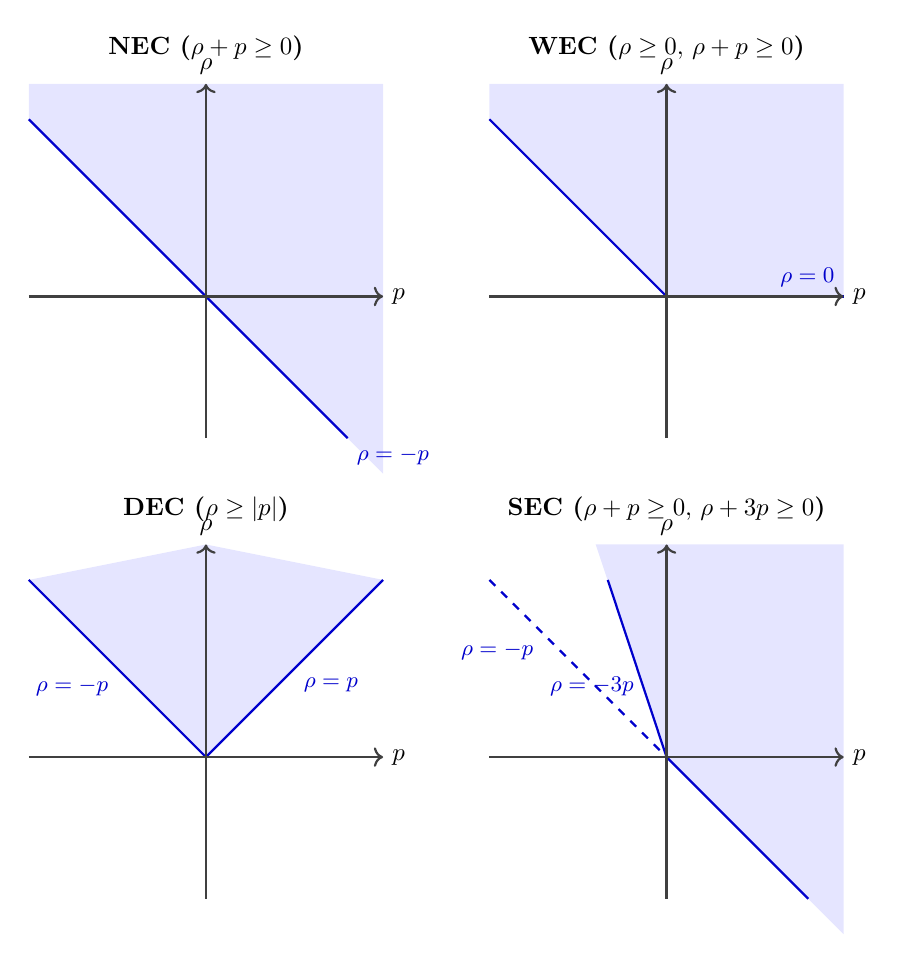
\begin{tikzpicture}[scale=0.9, every node/.style={scale=0.9}]
  % Common axes macro
  \def\drawaxes{
    \draw[->, thick, darkgray] (-2.5,0) -- (2.5,0) node[right, text=black] {$p$};
    \draw[->, thick, darkgray] (0,-2) -- (0,3) node[above, text=black] {$\rho$};
  }

  % NEC (Null Energy Condition)
  \begin{scope}[shift={(0, 6.5)}]
    \fill[blue!10] (-2.5, 2.5) -- (2.5, -2.5) -- (2.5, 3) -- (-2.5, 3) -- cycle;
    \draw[thick, blue!80!black] (-2.5, 2.5) -- (2.0, -2.0) node[below right, font=\small] {$\rho = -p$};
    \drawaxes
    \node[font=\bfseries] at (0, 3.5) {NEC ($\rho + p \ge 0$)};
  \end{scope}

  % WEC (Weak Energy Condition)
  \begin{scope}[shift={(6.5, 6.5)}]
    \fill[blue!10] (-2.5, 2.5) -- (0, 0) -- (2.5, 0) -- (2.5, 3) -- (-2.5, 3) -- cycle;
    \draw[thick, blue!80!black] (-2.5, 2.5) -- (0, 0);
    \draw[thick, blue!80!black] (0, 0) -- (2.5, 0) node[above left, font=\small] {$\rho = 0$};
    \drawaxes
    \node[font=\bfseries] at (0, 3.5) {WEC ($\rho \ge 0, \, \rho + p \ge 0$)};
  \end{scope}

  % DEC (Dominant Energy Condition)
  \begin{scope}[shift={(0, 0)}]
    \fill[blue!10] (0,0) -- (2.5, 2.5) -- (0, 3) -- (-2.5, 2.5) -- cycle;
    \draw[thick, blue!80!black] (-2.5, 2.5) -- (0, 0) node[midway, below left, font=\small] {$\rho = -p$};
    \draw[thick, blue!80!black] (0, 0) -- (2.5, 2.5) node[midway, below right, font=\small] {$\rho = p$};
    \drawaxes
    \node[font=\bfseries] at (0, 3.5) {DEC ($\rho \ge |p|$)};
  \end{scope}

  % SEC (Strong Energy Condition)
  \begin{scope}[shift={(6.5, 0)}]
    \fill[blue!10] (-1.0, 3) -- (0,0) -- (2.5, -2.5) -- (2.5, 3) -- cycle;
    \draw[thick, blue!80!black, dashed] (-2.5, 2.5) -- (0, 0) node[pos=0.3, below left, font=\small] {$\rho = -p$};
    \draw[thick, blue!80!black] (-0.83, 2.5) -- (0, 0) node[pos=0.6, left, font=\small] {$\rho = -3p$};
    \draw[thick, blue!80!black] (0,0) -- (2.0, -2.0);
    \drawaxes
    \node[font=\bfseries] at (0, 3.5) {SEC ($\rho + p \ge 0, \, \rho + 3p \ge 0$)};
  \end{scope}
\end{tikzpicture}
\caption{The four standard energy conditions in General Relativity.}
\label{fig:energy_conditions}
\end{figure}


\section{The Equivalence Principle Revisited}
The strict enforcement of the minimal-coupling principle is technically an approximation. While applying the "comma-goes-to-semicolon" rule to a flat-space Lagrangian reliably generates the minimally coupled action, the true physical action could theoretically include explicit non-minimal couplings between matter fields and the Ricci scalar (parameterized by $\xi$) that identically vanish in the flat-space limit:
\begin{equation}
\label{eq:minimal_scalar}
S_{\text{min}} = \int d^{4}x \sqrt{-g} \left[ -\frac{1}{2} g^{\mu\nu} \nabla_{\mu}\phi \nabla_{\nu}\phi - \frac{1}{2}m^{2}\phi^{2} \right]
\end{equation}
\begin{equation}
\label{eq:nonminimal_scalar}
S_{\text{non-min}} = \int d^{4}x \sqrt{-g} \left[ \frac{1}{2} \xi R \phi^{2} \right]
\end{equation}

\section{Alternative Theories of Gravity}
\subsection{Higher-Order Actions: $f(R)$ Gravity}
Einstein's theory restricts the gravitational Lagrangian strictly to the linear scalar curvature $R$. Broadening this action to encompass arbitrary analytical functions of the Ricci scalar, $f(R)$, constructs higher-order modifications to gravity:
\begin{equation}
\label{eq:fR_action}
S = \int d^{4}x \sqrt{-g} \left[ \frac{1}{16\pi G} f(R) + \mathcal{L}_{M} \right]
\end{equation}
By executing a functional variation of this modified action with respect to the metric, taking explicit care to properly integrate the second-order derivative variations $\delta R_{\mu\nu}$ via the generalized Palatini equation \eqref{eq:palatini_contracted}, the foundational equations of $f(R)$ gravity emerge, exhibiting dynamic self-coupling behaviors analogous to a scalar field:
\begin{equation}
\label{eq:fR_field_equation}
f'(R)R_{\mu\nu} - \frac{1}{2}f(R)g_{\mu\nu} + \left( \nabla_{\mu}\nabla_{\nu} - g_{\mu\nu}\Box \right) f'(R) = 8\pi G T_{\mu\nu}
\end{equation}

\subsection{Scalar-Tensor Theories and Torsion}
Further geometric expansions involve integrating standalone dynamic scalar fields $\phi$ that interact directly with the curvature tensor, typified by Brans-Dicke theory:
\begin{equation}
S = \int d^{4}x \sqrt{-g} \left[ \phi R - \frac{\omega(\phi)}{\phi} g^{\mu\nu}\nabla_{\mu}\phi\nabla_{\nu}\phi - V(\phi) + \mathcal{L}_{M} \right]
\end{equation}
Additionally, relaxing the symmetry condition of the Levi-Civita connection formally permits the introduction of spacetime Torsion, mathematically codified as the antisymmetric component of the connection array:
\begin{equation}
T^{\rho}_{\ \mu\nu} = \Gamma^{\rho}_{\mu\nu} - \Gamma^{\rho}_{\nu\mu}
\end{equation}

\section{Variational Derivations of Advanced Field Equations}
\subsection{The Electromagnetic Stress-Energy Tensor}
The formal integration of electromagnetism into the curved manifold is strictly governed by the minimally-coupled Maxwell action:
\begin{equation}
\label{eq:em_action}
S_{\text{EM}} = \int d^{4}x \sqrt{-g} \left( -\frac{1}{4} F^{\mu\nu}F_{\mu\nu} + A_{\mu}J^{\mu} \right)
\end{equation}
By systematically varying this action strictly with respect to the fundamental metric $g^{\mu\nu}$, and functionally isolating the metric dependence embedded inherently within the raised indices of the invariant field strength tensor product $F^{\mu\nu}F_{\mu\nu}$, the explicit, rigorously symmetric, and trace-free electromagnetic stress-energy tensor is successfully recovered:
\begin{equation}
\label{eq:em_tensor_derived}
T_{\rho\sigma} = F_{\rho\lambda}F_{\sigma}^{\ \lambda} - \frac{1}{4} g_{\rho\sigma} F_{\mu\nu}F^{\mu\nu}
\end{equation}

\chapter{The Schwarzschild Solution}

\section{The Schwarzschild Solution}

\subsection{Metric Ansatz and Symmetry Justification}
To rigorously describe the exterior gravitational field of a static, spherically symmetric mass distribution, we establish a metric ansatz starting from the geometry of flat Minkowski space:
\begin{equation}
ds_{\text{Minkowski}}^2 = -dt^2 + dr^2 + r^2 d\Omega^2, \quad \text{where} \quad d\Omega^2 = d\theta^2 + \sin^2\theta \, d\phi^2.
\end{equation}
Physical staticity requires that the metric components possess no explicit time dependence and remain strictly invariant under time reversal ($t \rightarrow -t$). This invariance geometrically prohibits the existence of any cross terms involving $dt$, dictating that $g_{ti} = 0$. 

Spherical symmetry further constrains the angular dependence entirely to the standard $d\Omega^2$ element. To mathematically guarantee a valid Lorentzian signature across the manifold, the remaining unknown metric components are conventionally expressed as positive exponentials:
\begin{equation}
ds^2 = -e^{2\alpha(r)} dt^2 + e^{2\beta(r)} dr^2 + e^{2\gamma(r)} r^2 d\Omega^2.
\end{equation}
By exploiting the inherent coordinate freedom of general relativity, we define a new radial coordinate $\overline{r} = e^{\gamma(r)} r$. Applying this transformation completely absorbs the conformal angular factor $e^{2\gamma(r)}$. Dropping the overbars for notational simplicity yields the canonical, diagonal metric ansatz for a static, spherically symmetric spacetime:
\begin{equation}
ds^2 = -e^{2\alpha(r)} dt^2 + e^{2\beta(r)} dr^2 + r^2 d\Omega^2.
\end{equation}

\subsection{Inverse Metric and Determinant}
The covariant components of the metric tensor are read directly from the line element. Because the metric is manifestly orthogonal (diagonal), the computation of the contravariant inverse metric $g^{\mu\nu}$ circumvents complex matrix inversion; the non-zero components are strictly the reciprocals of the covariant components:
\begin{equation}
g_{\mu\nu} = \text{diag}\left(-e^{2\alpha(r)}, e^{2\beta(r)}, r^2, r^2 \sin^2\theta\right),
\end{equation}
\begin{equation}
g^{\mu\nu} = \text{diag}\left(-e^{-2\alpha(r)}, e^{-2\beta(r)}, \frac{1}{r^2}, \frac{1}{r^2 \sin^2\theta}\right).
\end{equation}
The invariant volume element, essential for integration over the curved manifold, relies on the metric determinant $g$. Multiplying the diagonal elements and extracting the square root analytically yields:
\begin{equation}
g = - e^{2(\alpha(r) + \beta(r))} r^4 \sin^2\theta \quad \implies \quad \sqrt{-g} = e^{\alpha(r) + \beta(r)} r^2 \sin\theta.
\end{equation}

\subsection{Deriving Christoffel Symbols via the Lagrangian Method}
Rather than calculating the connection coefficients directly from metric derivatives, it is computationally more elegant to extract them via the variational principle. By defining the Lagrangian $\mathcal{L} = g_{\mu\nu} \dot{x}^\mu \dot{x}^\nu$ and applying the Euler-Lagrange equations, the resulting equations of motion natively mirror the geodesic equation:
\begin{equation}
\frac{d}{d\lambda} \left( \frac{\partial \mathcal{L}}{\partial \dot{x}^\mu} \right) - \frac{\partial \mathcal{L}}{\partial x^\mu} = 0 \quad \implies \quad \ddot{x}^\mu + \Gamma^\mu_{\rho\sigma} \dot{x}^\rho \dot{x}^\sigma = 0. \label{eq:EL_general}
\end{equation}

By systematically evaluating the Euler-Lagrange equations for the $t$, $r$, $\theta$, and $\phi$ coordinates and factoring out the quadratic velocity terms, we isolate the non-vanishing Christoffel symbols. For the strictly static metric ($\partial_t \alpha = \partial_t \beta = 0$), the non-zero connection coefficients are:
\begin{align}
\Gamma^t_{tr} &= \partial_r \alpha, \\
\Gamma^r_{tt} &= e^{2(\alpha - \beta)} \partial_r \alpha, \\
\Gamma^r_{rr} &= \partial_r \beta, \\
\Gamma^r_{\theta\theta} &= -r e^{-2\beta}, \\
\Gamma^r_{\phi\phi} &= -r e^{-2\beta} \sin^2\theta, \\
\Gamma^\theta_{r\theta} &= \frac{1}{r}, \\
\Gamma^\theta_{\phi\phi} &= -\sin\theta \cos\theta, \\
\Gamma^\phi_{r\phi} &= \frac{1}{r}, \\
\Gamma^\phi_{\theta\phi} &= \cot\theta.
\end{align}

\subsection{Derivation of the Ricci Tensor}
The physical curvature of the spacetime is locally quantified by the Ricci tensor, $R_{\mu\nu}$. Substituting the derived Christoffel symbols into the general definition of the Ricci tensor and systematically contracting indices produces the diagonal curvature components:
\begin{equation}
R_{\mu\nu} = \partial_\lambda \Gamma^\lambda_{\mu\nu} - \partial_\nu \Gamma^\lambda_{\mu\lambda} + \Gamma^\lambda_{\sigma\lambda} \Gamma^\sigma_{\mu\nu} - \Gamma^\lambda_{\sigma\nu} \Gamma^\sigma_{\mu\lambda}.
\end{equation}
Executing these differential operations yields the following non-vanishing components:
\begin{align}
R_{tt} &= e^{2(\alpha-\beta)} \left[ \partial_r^2\alpha + (\partial_r\alpha)^2 - \partial_r\alpha\partial_r\beta + \frac{2}{r}\partial_r\alpha \right], \\
R_{rr} &= -\partial_r^2\alpha - (\partial_r\alpha)^2 + \partial_r\alpha\partial_r\beta + \frac{2}{r}\partial_r\beta, \\
R_{\theta\theta} &= e^{-2\beta} \left[ r(\partial_r\beta - \partial_r\alpha) - 1 \right] + 1, \\
R_{\phi\phi} &= \sin^2\theta \left[ e^{-2\beta} \left( r\partial_r\beta - r\partial_r\alpha - 1 \right) + 1 \right].
\end{align}

\subsection{Einstein Equations and Solution}
To describe the exterior vacuum region surrounding the mass, we enforce the vacuum Einstein field equations, $R_{\mu\nu} = 0$. 

By observing the structural similarities between $R_{tt}$ and $R_{rr}$, taking the linear combination $e^{2(\beta-\alpha)} R_{tt} + R_{rr} = 0$ radically simplifies the coupled differential equations:
\begin{equation}
\frac{2}{r} \left( \partial_r\alpha + \partial_r\beta \right) = 0 \quad \implies \quad \alpha(r) + \beta(r) = c.
\end{equation}
Absorbing the integration constant into a global time rescaling allows us to set $\beta(r) = -\alpha(r)$. Substituting this symmetry back into the angular curvature equation $R_{\theta\theta} = 0$ reduces it to an exact total derivative:
\begin{equation}
\partial_r \left( r e^{2\alpha} \right) = 1 \quad \implies \quad e^{2\alpha(r)} = 1 + \frac{C_1}{r}.
\end{equation}

\subsection{Final Schwarzschild Metric and Interpretation}
To determine the physical meaning of the integration constant $C_1$, we require the resulting metric to smoothly recover the weak-field Newtonian potential $\Phi = -GM/r$ at large distances. In this limit, $g_{tt} \approx -(1 + 2\Phi)$, which fixes the constant as the Schwarzschild radius, $R_S = 2GM$:
\begin{equation}
-\left( 1 + \frac{C_1}{r} \right) = -\left( 1 - \frac{2GM}{r} \right) \quad \implies \quad C_1 = -2GM.
\end{equation}
The unique, exact solution for the geometry outside a spherically symmetric mass is the Schwarzschild metric:
\begin{equation}
ds^2 = -\left( 1 - \frac{2GM}{r} \right) dt^2 + \left( 1 - \frac{2GM}{r} \right)^{-1} dr^2 + r^2 d\Omega^2.
\end{equation}

\section{Birkhoff's Theorem}
Birkhoff's theorem states a profound uniqueness property of general relativity: any spherically symmetric solution to the vacuum field equations must necessarily be static and asymptotically flat. Thus, the Schwarzschild metric is the unique exterior solution even for a pulsating or collapsing star.

Starting with the most general spherically symmetric metric permitted by the geometric coordinates $(a, b)$:
\begin{equation}
ds^{2} = g_{aa}(a,b)da^{2} + 2g_{ab}(a,b)da db + g_{bb}(a,b)db^{2} + r^{2}(a,b)d\Omega^{2}.
\end{equation}
By performing a sequence of coordinate transformations to establish a true radial coordinate $r$ and diagonalize the temporal-radial subspace into a generic time coordinate $t$, the metric assumes the pre-static form:
\begin{equation}
ds^{2} = -e^{2\alpha(t,r)}dt^{2} + e^{2\beta(t,r)}dr^{2} + r^{2}d\Omega^{2}.
\end{equation}
Imposing the vacuum equations $R_{\mu\nu} = 0$ on this time-dependent metric mandates that $\partial_t \beta = 0$, meaning $\beta$ is strictly a function of $r$. Subsequent evaluation of $R_{\theta\theta}=0$ forces the cross-derivative of $\alpha$ to vanish, proving the time dependence is entirely separable ($\alpha(t,r) = f(r) + g(t)$). By redefining the time coordinate to absorb $g(t)$, the metric fundamentally reverts to the static Schwarzschild form.

\section{Coordinate vs. Curvature Singularities}
The Schwarzschild metric exhibits apparent infinities at $r=2GM$ and $r=0$. To distinguish between artifacts of our coordinate choice and genuine physical breakdowns in the manifold, we evaluate a completely coordinate-invariant geometric scalar, the Kretschmann scalar $K = R^{\mu\nu\rho\sigma}R_{\mu\nu\rho\sigma}$. 

Computing this contraction for the Schwarzschild geometry yields:
\begin{equation}
K = \frac{48G^{2}M^{2}}{r^{6}}.
\end{equation}
As $r \to 0$, $K$ diverges to infinity, definitively identifying the origin as a true, inescapable curvature singularity where tidal forces become infinite. However, at the Schwarzschild radius:
\begin{equation}
K(r=2GM) = \frac{3}{4G^{4}M^{4}}.
\end{equation}
Because the scalar remains finite, $r=2GM$ is merely a coordinate singularity; spacetime is perfectly smooth and physically traversable at this location, though the choice of $(t,r)$ coordinates fails.

\section{Geodesics of the Schwarzschild Geometry}
To analyze particle motion, we exploit the continuous symmetries of the Schwarzschild spacetime. Time translation invariance and azimuthal rotational invariance naturally yield two conserved quantities—energy $E$ and angular momentum $L$—which greatly simplify the integration of the geodesic equations.
\begin{align}
E &= \left(1-\frac{2GM}{r}\right)\frac{dt}{d\lambda}, \label{eq:energy_conserved} \\
L &= r^{2} \frac{d\phi}{d\lambda}. \label{eq:angular_conserved}
\end{align}
Restricting motion to the equatorial plane ($\theta = \pi/2$) without loss of generality, and utilizing the four-velocity normalization $g_{\mu\nu}\dot{x}^\mu \dot{x}^\nu = -\epsilon$ (where $\epsilon=1$ for massive particles and $\epsilon=0$ for photons), we obtain the fundamental radial energy equation:
\begin{equation}
\label{eq:radial_energy_eq}
\frac{1}{2}\left(\frac{dr}{d\lambda}\right)^{2} + V_{\text{eff}}(r) = \frac{1}{2}E^2, \quad \text{where} \quad V_{\text{eff}}(r) = \frac{1}{2}\epsilon - \epsilon\frac{GM}{r} + \frac{L^{2}}{2r^{2}} - \frac{GML^{2}}{r^{3}}.
\end{equation}


% Drawing 5: Effective Potential for a Massive Particle
\begin{figure}[htbp]
\centering
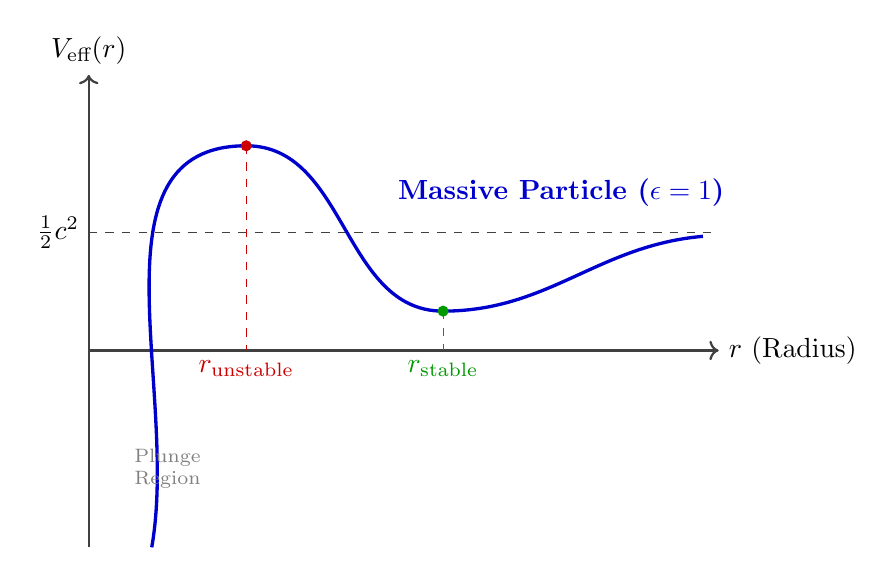
\begin{tikzpicture}[scale=1.0]
  % Axes
  \draw[->, thick, darkgray] (0,-2.5) -- (0, 3.5) node[above, text=black] {$V_{\text{eff}}(r)$};
  \draw[->, thick, darkgray] (0,0) -- (8, 0) node[right, text=black] {$r$ (Radius)};
  
  % Asymptote for massive particles (E_rest / m c^2)
  \draw[dashed, darkgray] (0, 1.5) node[left, text=black] {$\frac{1}{2}c^2$} -- (8, 1.5);

  % Extrema Coordinates
  \coordinate (Peak) at (2.0, 2.6);
  \coordinate (Min) at (4.5, 0.5);

  % The Effective Potential Curve (Massive Particle)
  \draw[very thick, blue!80!black] (0.8, -2.5)
    to[out=80, in=180] (Peak)
    to[out=0, in=180] (Min)
    to[out=0, in=185] (7.8, 1.45);
    
  % Annotations for Extrema
  \draw[dashed, red!80!black] (Peak) -- (2.0, 0) node[below] {$r_{\text{unstable}}$};
  \draw[dashed, green!60!black] (Min) -- (4.5, 0) node[below] {$r_{\text{stable}}$};
  
  \fill[red!80!black] (Peak) circle (2pt);
  \fill[green!60!black] (Min) circle (2pt);

  % Add a label for the curve
  \node[blue!80!black, font=\bfseries] at (6, 2.0) {Massive Particle ($\epsilon=1$)};
  
  % Singularity Region
  \node[align=center, font=\scriptsize, gray] at (1.0, -1.5) {Plunge \\ Region};
\end{tikzpicture}
\caption{Effective potential profile for a massive particle.}
\label{fig:effective_potential}
\end{figure}

By evaluating the roots of the potential's derivative ($dV_{\text{eff}}/dr = 0$), we locate circular orbits. For photons ($\epsilon=0$), there exists exactly one unstable circular orbit (the photon sphere) at $r_c = 3GM$. 
For massive particles ($\epsilon=1$), circular orbits exist at:
\begin{equation}
\label{eq:circular_radii}
r_{c} = \frac{L^{2} \pm \sqrt{L^{4} - 12G^{2}M^{2}L^{2}}}{2GM}.
\end{equation}
The geometry strictly forbids stable orbits infinitely close to the horizon; the Innermost Stable Circular Orbit (ISCO) occurs at $r_{\text{ISCO}} = 6GM$.

\section{Experimental Tests of General Relativity}
\subsection{The Precession of Perihelia}
To map the shape of planetary orbits, we transform the radial time-evolution equation into a geometric equation parameterized by the azimuthal angle $\phi$. Applying the substitution $u = 1/r$ transforms the energy equation into a non-linear differential equation describing the orbital trajectory:
\begin{equation}
\frac{d^{2}u}{d\phi^{2}} + u = \frac{GM}{L^{2}} + 3GMu^{2}.
\end{equation}
The final non-linear term is a purely relativistic correction to Newtonian dynamics. By scaling the variables to a dimensionless form $x = L^2 u / GM$ and performing a perturbative expansion ($x = x_0 + x_1$), we iteratively solve for the modified orbital path:
\begin{equation}
\label{eq:precession_phase}
x(\phi) \approx 1 + e \cos[(1-\alpha)\phi].
\end{equation}


% Drawing 6: Precession of Bound Orbits
\begin{figure}[htbp]
\centering
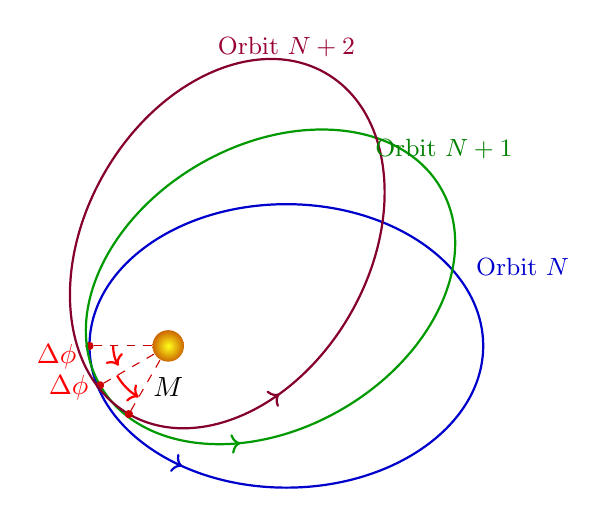
\begin{tikzpicture}[scale=1.0]
  \coordinate (O) at (0,0);

  % Orbit 1 (Initial)
  \begin{scope}[rotate=0]
    \draw[thick, blue!80!black, decoration={markings, mark=at position 0.65 with {\arrow{>}}}, postaction={decorate}] (1.5, 0) ellipse (2.5 and 1.8);
    \draw[dashed, red!80!black] (O) -- (-1, 0) coordinate (P1);
    \fill[red!80!black] (-1,0) circle (1.5pt);
  \end{scope}

  % Orbit 2 (Precessed)
  \begin{scope}[rotate=30]
    \draw[thick, green!60!black, decoration={markings, mark=at position 0.65 with {\arrow{>}}}, postaction={decorate}] (1.5, 0) ellipse (2.5 and 1.8);
    \draw[dashed, red!80!black] (O) -- (-1, 0) coordinate (P2);
    \fill[red!80!black] (-1,0) circle (1.5pt);
  \end{scope}
  
  % Orbit 3 (Further Precessed)
  \begin{scope}[rotate=60]
    \draw[thick, purple!70!black, decoration={markings, mark=at position 0.65 with {\arrow{>}}}, postaction={decorate}] (1.5, 0) ellipse (2.5 and 1.8);
    \draw[dashed, red!80!black] (O) -- (-1, 0) coordinate (P3);
    \fill[red!80!black] (-1,0) circle (1.5pt);
  \end{scope}

  % Central mass (Sun/Black Hole)
  \shade[inner color=yellow!90!white, outer color=orange!80!black] (O) circle (0.2) node[below=8pt, text=black, font=\bfseries] {$M$};

  % Precession angle arcs
  \draw[->, thick, red] (-0.7, 0) arc (180:210:0.5) node[midway, left=10pt] {$\Delta\phi$};
  \draw[->, thick, red] (-0.65, -0.375) arc (210:240:0.75) node[midway, left=10pt] {$\Delta\phi$};

  % Legend / Labels
  \node[blue!80!black, font=\small] at (4.5, 1.0) {Orbit $N$};
  \node[green!50!black, font=\small] at (3.5, 2.5) {Orbit $N+1$};
  \node[purple!80!black, font=\small] at (1.5, 3.8) {Orbit $N+2$};

\end{tikzpicture}
\caption{Orbital precession around a central mass.}
\label{fig:orbital_precession}
\end{figure}

Because the angular frequency is no longer perfectly commensurate with the radial frequency, the orbital ellipse fails to close, instead smoothly precessing by an angle $\Delta\phi$ each revolution:
\begin{equation}
\Delta\phi = \frac{6\pi GM}{c^{2}a(1-e^{2})} \text{ radians per orbit}.
\end{equation}

\subsection{Gravitational Redshift}
A stationary observer positioned deep in a gravitational well evaluates physical frequencies using their local proper time. By tracking the projection of a photon's four-momentum onto the observer's four-velocity, we calculate the observed frequency ratio between two separated observers:
\begin{equation}
\frac{\omega_{2}}{\omega_{1}} = \left( \frac{1-\frac{2GM}{r_{1}}}{1-\frac{2GM}{r_{2}}} \right)^{1/2}.
\end{equation}
Expanding this expression into the weak-field Newtonian limit rigorously confirms that photons lose energy as they climb out of a potential well:
\begin{equation}
\frac{\omega_{2}}{\omega_{1}} \approx 1 + \Phi(r_{1}) - \Phi(r_{2}) = 1 - \Delta\Phi.
\end{equation}

\section{Schwarzschild Black Holes and Causal Structure}
\subsection{Causal Structure in Schwarzschild Coordinates}
By analyzing radial light rays ($ds^2 = 0, d\Omega^2 = 0$), we determine the slope of light cones in a standard Schwarzschild $t-r$ diagram:
\begin{equation}
\label{eq:radial_light_cone}
\frac{dt}{dr} = \pm \left( 1 - \frac{2GM}{r} \right)^{-1}.
\end{equation}
As an observer approaches the Schwarzschild radius, the light cone slopes asymptotically approach infinity, suggesting that light is frozen at the boundary.


% Drawing 7: Light Cones Narrowing (Schwarzschild Coordinates)
\begin{figure}[htbp]
\centering
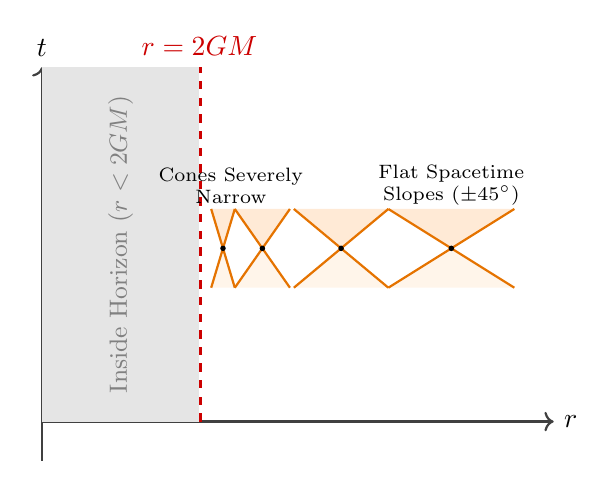
\begin{tikzpicture}[scale=1.0]
  % Axes
  \draw[->, thick, darkgray] (0,-0.5) -- (0, 4.5) node[above, text=black] {$t$};
  \draw[->, thick, darkgray] (0,0) -- (6.5, 0) node[right, text=black] {$r$};

  % Horizon line
  \draw[ultra thick, dashed, red!80!black] (2.0, 0) -- (2.0, 4.5) node[above] {$r = 2GM$};
  
  % Singularity placeholder shaded area
  \fill[gray!20] (0,0) rectangle (2.0, 4.5);
  \node[rotate=90, gray, font=\small] at (1.0, 2.25) {Inside Horizon ($r < 2GM$)};

  % Light cones macro
  \newcommand{\schwarzschildcone}[3]{
    % #1: center x, #2: center y, #3: width (dt/dr slope factor)
    \begin{scope}[shift={(#1,#2)}]
      \fill[orange!20, opacity=0.8] (0,0) -- (-#3, 0.5) -- (#3, 0.5) -- cycle;
      \fill[orange!10, opacity=0.8] (0,0) -- (-#3, -0.5) -- (#3, -0.5) -- cycle;
      \draw[thick, orange!90!black] (-#3, -0.5) -- (#3, 0.5);
      \draw[thick, orange!90!black] (#3, -0.5) -- (-#3, 0.5);
      \fill[black] (0,0) circle (1pt);
    \end{scope}
  }

  % Draw light cones at different radii
  % As r -> 2GM, dt/dr -> infinity, so the cone becomes extremely narrow in space (x-width decreases)
  \schwarzschildcone{2.3}{2.2}{0.15}
  \schwarzschildcone{2.8}{2.2}{0.35}
  \schwarzschildcone{3.8}{2.2}{0.6}
  \schwarzschildcone{5.2}{2.2}{0.8}

  % Labels
  \node[font=\scriptsize, align=center] at (5.2, 3.0) {Flat Spacetime \\ Slopes ($\pm 45^\circ$)};
  \node[font=\scriptsize, align=center] at (2.4, 3.0) {Cones Severely \\ Narrow};

\end{tikzpicture}
\caption{Light cones narrowing near the horizon in Schwarzschild coordinates.}
\label{fig:lightcones_schwarzschild}
\end{figure}


\subsection{The Tortoise Coordinate}
Because the divergence at $r=2GM$ is merely a coordinate failure, we construct a new spatial coordinate mapping $r \to r^*$ that stretches the horizon to asymptotic infinity, effectively un-kinking the null trajectories. Integrating the null condition identifies the Tortoise coordinate:
\begin{equation}
\label{eq:tortoise_def}
r^{*} \equiv r + 2GM \ln\left| \frac{r}{2GM} - 1 \right|.
\end{equation}

\subsection{Eddington-Finkelstein Coordinates}
To forge a coordinate system that remains mathematically regular directly across the horizon, we utilize the advanced time coordinate $v$, defined as a constant along ingoing light rays:
\begin{equation}
\label{eq:advanced_v}
v \equiv t + r^{*}.
\end{equation}
Substituting this substitution into the metric effectively eliminates the singular diagonal divergence, resulting in the regular Eddington-Finkelstein geometry:
\begin{equation}
\label{eq:eddington_metric}
ds^{2} = -\left( 1 - \frac{2GM}{r} \right)dv^{2} + 2 dv dr + r^{2} d\Omega^{2}.
\end{equation}
Computing the determinant ($g = -r^{4}\sin^{2}\theta$) confirms that the metric behaves perfectly smoothly across $r=2GM$.

\subsection{The Event Horizon and the Tipping of Light Cones}
In Eddington-Finkelstein coordinates, the local causal structure becomes transparently physical. Evaluating the slopes of the null curves $dv/dr$:
\begin{align}
\text{Ingoing null geodesics: } \quad &\frac{dv}{dr} = 0 \quad \implies \quad v = \text{constant}, \\
\text{Outgoing null geodesics: } \quad &\frac{dv}{dr} = 2 \left( 1 - \frac{2GM}{r} \right)^{-1}.
\end{align}

% Drawing 8: Light Cones Tipping (Eddington-Finkelstein Coordinates)
\begin{figure}[htbp]
\centering
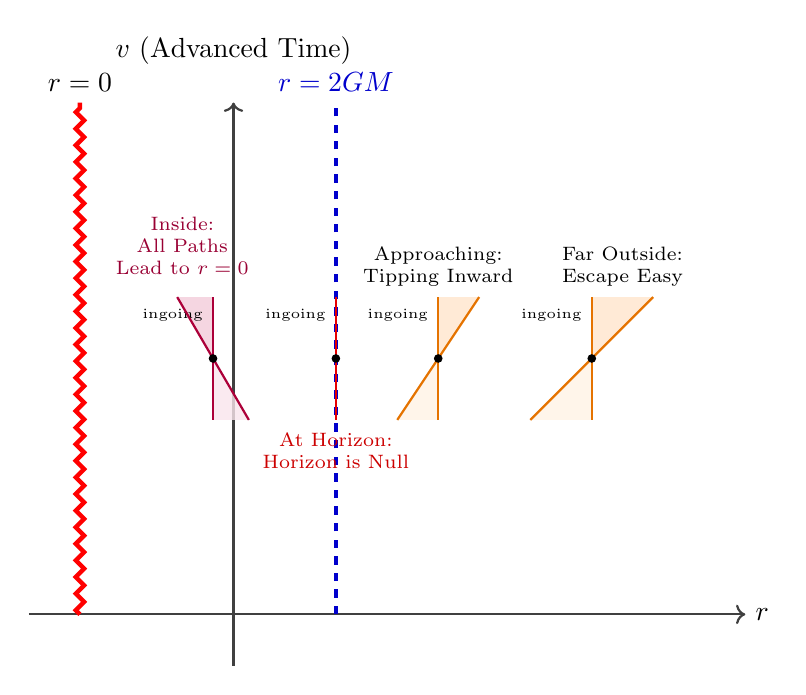
\begin{tikzpicture}[scale=1.3]
  % Axes
  \draw[->, thick, darkgray] (2.0,-0.5) -- (2.0, 5) node[above=10pt, text=black] {$v$ (Advanced Time)};
  \draw[->, thick, darkgray] (0,0) -- (7, 0) node[right, text=black] {$r$};

  % Singularity at r=0
  \draw[ultra thick, decorate, decoration={zigzag, segment length=6pt, amplitude=1.5pt}, red] 
    (0.5, 0) -- (0.5, 5) node[above, text=black] {$r = 0$};

  % Event Horizon
  \draw[ultra thick, dashed, blue!80!black] (3.0, 0) -- (3.0, 5) node[above] {$r = 2GM$};

  % Light Cones Macro for EF Coordinates
  \newcommand{\efcone}[4]{
    \begin{scope}[shift={(#1,#2)}]
      \fill[#4!20, opacity=0.8] (0,0) -- (0, 0.6) -- (#3, 0.6) -- cycle;
      \fill[#4!10, opacity=0.8] (0,0) -- (0, -0.6) -- (-#3, -0.6) -- cycle;
      \draw[thick, #4!90!black] (0, -0.6) -- (0, 0.6) node[pos=0.85, left, font=\tiny, text=black] {ingoing};
      \draw[thick, #4!90!black] (-#3, -0.6) -- (#3, 0.6);
      \fill[black] (0,0) circle (1.2pt);
    \end{scope}
  }

  % Outside Horizon
  \efcone{5.5}{2.5}{0.6}{orange}
  \node[font=\scriptsize, align=center] at (5.8, 3.4) {Far Outside:\\Escape Easy};

  \efcone{4.0}{2.5}{0.4}{orange}
  \node[font=\scriptsize, align=center] at (4.0, 3.4) {Approaching:\\Tipping Inward};

  % At Horizon
  \efcone{3.0}{2.5}{0.0}{red}
  \node[red!80!black, font=\scriptsize, align=center] at (3.0, 1.6) {At Horizon:\\Horizon is Null};

  % Inside Horizon
  \efcone{1.8}{2.5}{-0.35}{purple}
  \node[purple!80!black, font=\scriptsize, align=center] at (1.5, 3.6) {Inside:\\All Paths\\Lead to $r=0$};

\end{tikzpicture}
\caption{Light cones tipping inward in Eddington-Finkelstein coordinates.}
\label{fig:lightcones_eddington_finkelstein}
\end{figure}

At exactly $r=2GM$, the outgoing branch becomes completely vertical, effectively making the horizon itself a null surface. For $r<2GM$, the "outgoing" slope becomes negative. The light cones have physically tipped over, ensuring that every possible future-directed timelike or null trajectory inevitably decreases in $r$ until terminating at the central singularity. This mathematically formalizes the boundary as an absolute Event Horizon.

% ==========================================
% CONCLUSION CHAPTER
% ==========================================

\chapter{Conclusion}

The development of general relativity stands as one of the crowning achievements of theoretical physics. By discarding the rigid, flat stage of Newtonian mechanics and replacing it with a dynamic, curved manifold, Einstein fundamentally altered our understanding of the universe. 
\newline

Throughout this thesis, we have traced the logical and mathematical architecture of this theory. We saw how the Equivalence Principle organically necessitated the use of differential geometry, forcing us to abandon flat-space partial derivatives in favor of connection coefficients and covariant derivatives. We quantified intrinsic curvature using the Riemann tensor, and we observed how the Einstein-Hilbert action elegantly unifies geometry and matter to yield the Einstein Field Equations. 
\newline

By applying this framework to the vacuum surrounding a spherical mass, we derived the Schwarzschild solution. This exact solution not only successfully predicts the minute anomalies in the orbit of Mercury and the gravitational redshift of light, but it also predicts the existence of regions where gravity becomes so intense that spacetime causally seals itself off from the rest of the universe—black holes. The shift in light cones described by Eddington-Finkelstein coordinates beautifully illustrates how, inside an event horizon, the progression of space and time forces all paths toward a central singularity.
\newline

Yet, despite its mathematical elegance and century-long streak of passing every experimental test, general relativity is not the final word in physics. The theory fundamentally predicts its own demise at singularities, where the curvature invariants formally diverge to infinity and classical predictability breaks down. The absolute necessity of a theory of Quantum Gravity—one that successfully reconciles the continuous, deterministic geometry of general relativity with the discrete, probabilistic nature of quantum mechanics—remains the greatest unsolved problem in modern theoretical physics. 
\newline

Furthermore, the recent cosmological discoveries of dark matter and dark energy—the latter often modeled as the cosmological constant $\Lambda$ introduced in our field equations—suggest that our understanding of the universe's energy-momentum tensor is remarkably incomplete. 
\newline

As we look to the future, propelled by the new era of multi-messenger astronomy and gravitational wave detection, the geometric framework detailed in this thesis will remain the bedrock upon which new physics is built. General relativity is more than just a theory of gravity; it is the definitive language of the cosmos.



\begin{thebibliography}{9}
\bibitem{carroll} 
Carroll, Sean M. \textit{Spacetime and Geometry: An Introduction to General Relativity}. Addison Wesley, 2004.
\bibitem{schutz} 
Schutz, Bernard F. \textit{A First Course in General Relativity}. Cambridge University Press, 2009.
\bibitem{wald} 
Wald, Robert M. \textit{General Relativity}. University of Chicago Press, 1984.
\bibitem{mtw}
Misner, C. W., Thorne, K. S., \& Wheeler, J. A. \textit{Gravitation}. W. H. Freeman, 1973.
\bibitem{hartle}
Hartle, James B. \textit{Gravity: An Introduction to Einstein's General Relativity}. Addison Wesley, 2003.
\end{thebibliography}

\end{document}